\documentclass[a4paper]{article}
\usepackage[14pt]{extsizes}
\usepackage[russian]{babel}
\usepackage[T2A]{fontenc}
\usepackage[utf8]{inputenc}
\usepackage{graphicx}
\usepackage{float}
\usepackage{enumitem}
\usepackage{indentfirst}
\linespread{1.25} 
\usepackage[left=3cm,right=1.5cm,top=2cm,bottom=2cm]{geometry}
\usepackage{tempora}                                     
\usepackage{newtxmath} 
\usepackage{titlesec}







\title{Установка и запуск PureVPN} 
\date{23 мая 2023 года}
\author{}

\begin{document}

\maketitle
\newpage
\tableofcontents
\newpage

\section{Windows}

\subsection{Загрузите приложение PureVPN} 
Воспользуйтесь видео-инструкцией https://clck.ru/34fMJC или:
\begin{itemize}
\item Перейдите по ссылке https://www.purevpn.com/download/windows-vpn, чтобы перейти на страницу загрузки приложения PureVPN.
\item Нажмите кнопку Загрузить приложение, чтобы загрузить приложение PureVPN на свое устройство:  Рисунок(\ref{fig:1})
\begin{figure}[H]
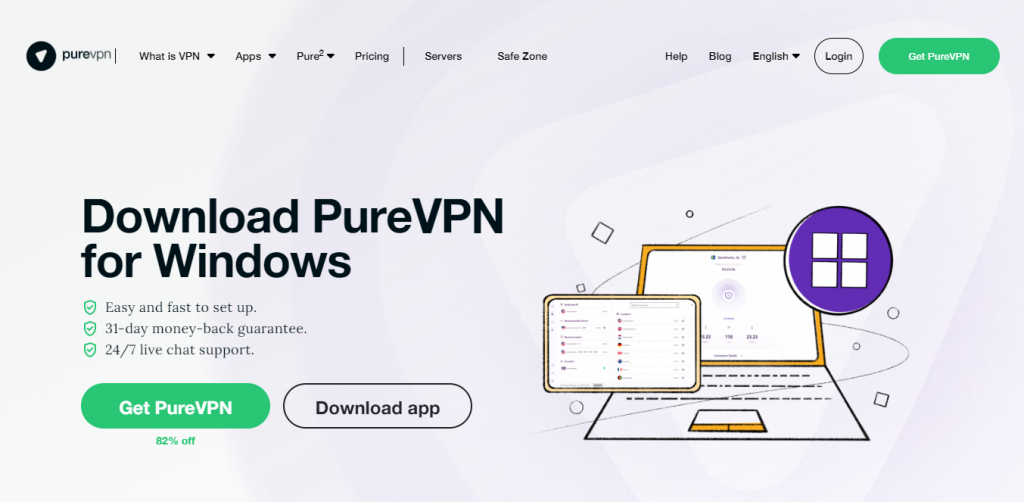
\includegraphics[width=14cm]{1.png}
\centering
\caption{Загрузить приложение}
\label{fig:1}
\end{figure}
\item После завершения загрузки найдите установочный файл на своем устройстве. Скорее всего, вы найдете его в папке Downloads вашего устройства.
\end{itemize}

\subsection{Установите приложение PureVPN} 
\begin{itemize}
\item Перейдите в папку загрузки вашего устройства и найдите PureVPN setup.exe
\item Дважды щелкните PureVPN setup.exe файл:  Рисунок(\ref{fig:2})
\begin{figure}[H]
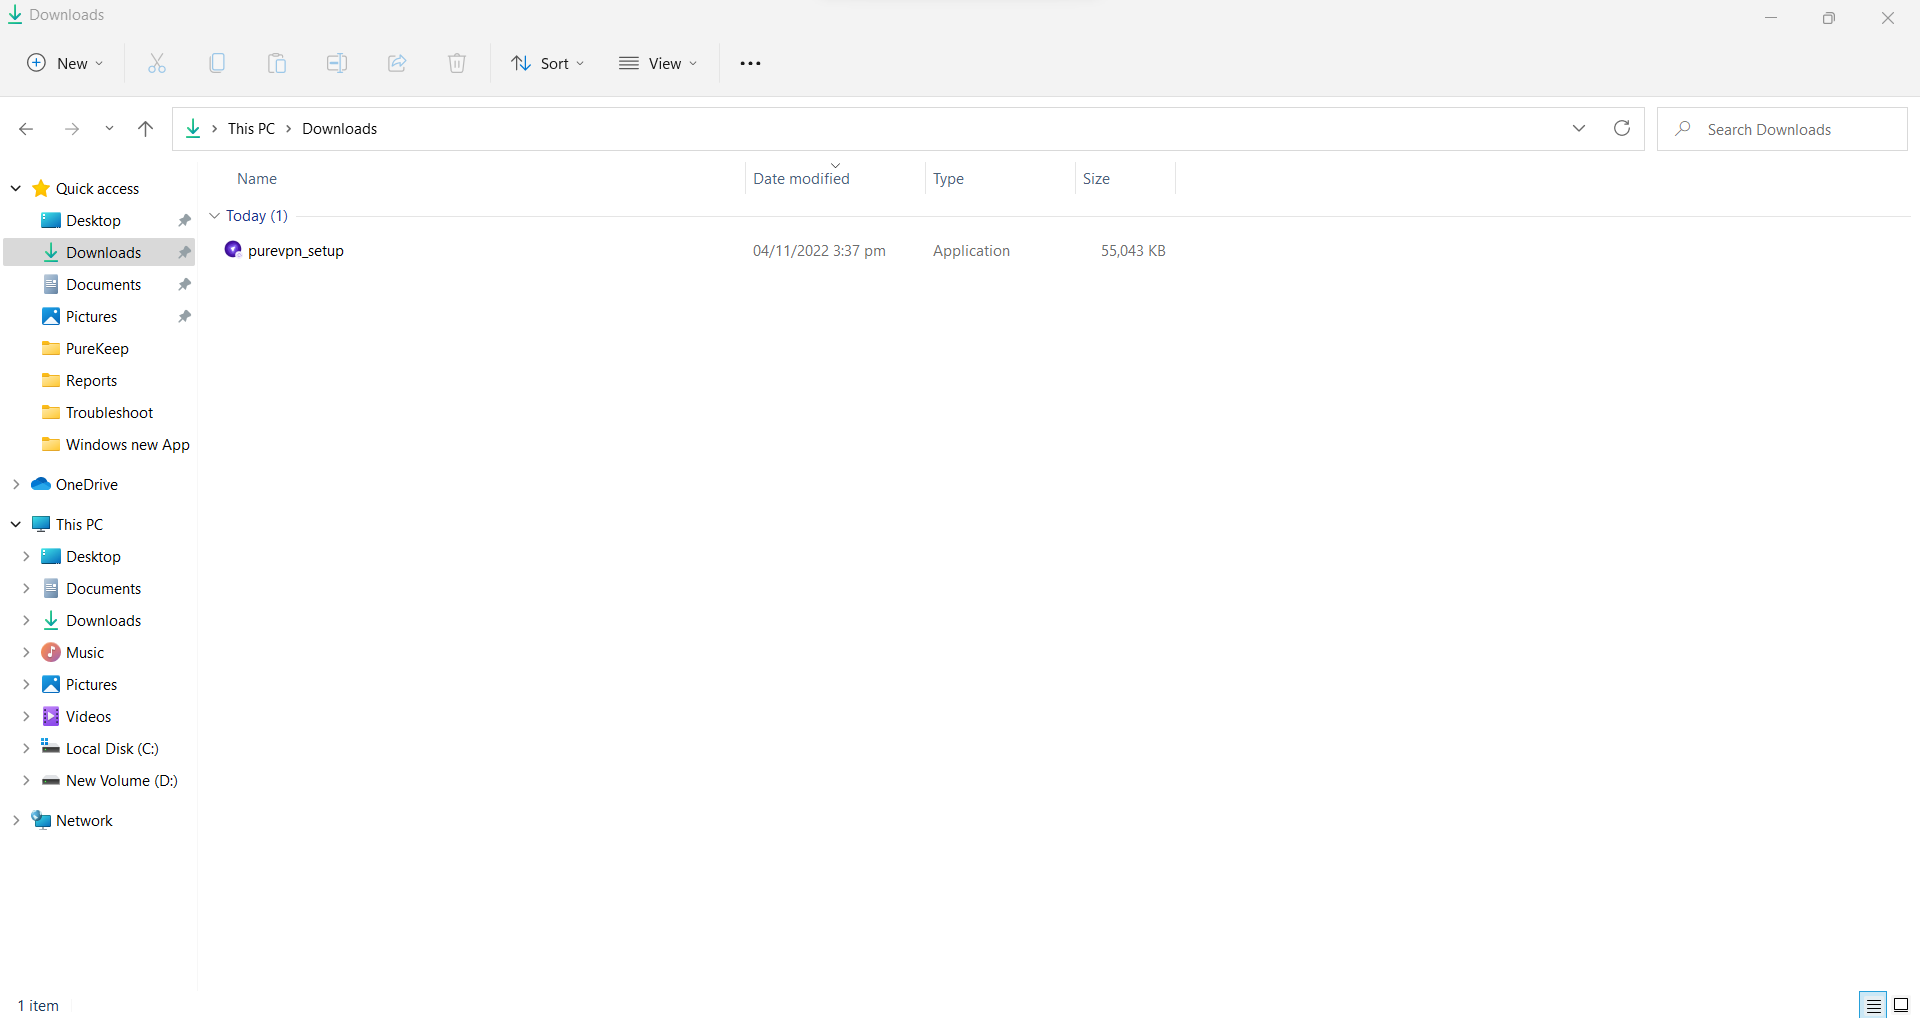
\includegraphics[width=14cm]{2.png}
\centering
\caption{PureVPN setup.exe}
\label{fig:2}
\end{figure}
\item Компьютер спросит, хотите ли вы разрешить этому приложению вносить изменения в ваше устройство? Нажмите Да:  Рисунок(\ref{fig:3})
\begin{figure}[H]
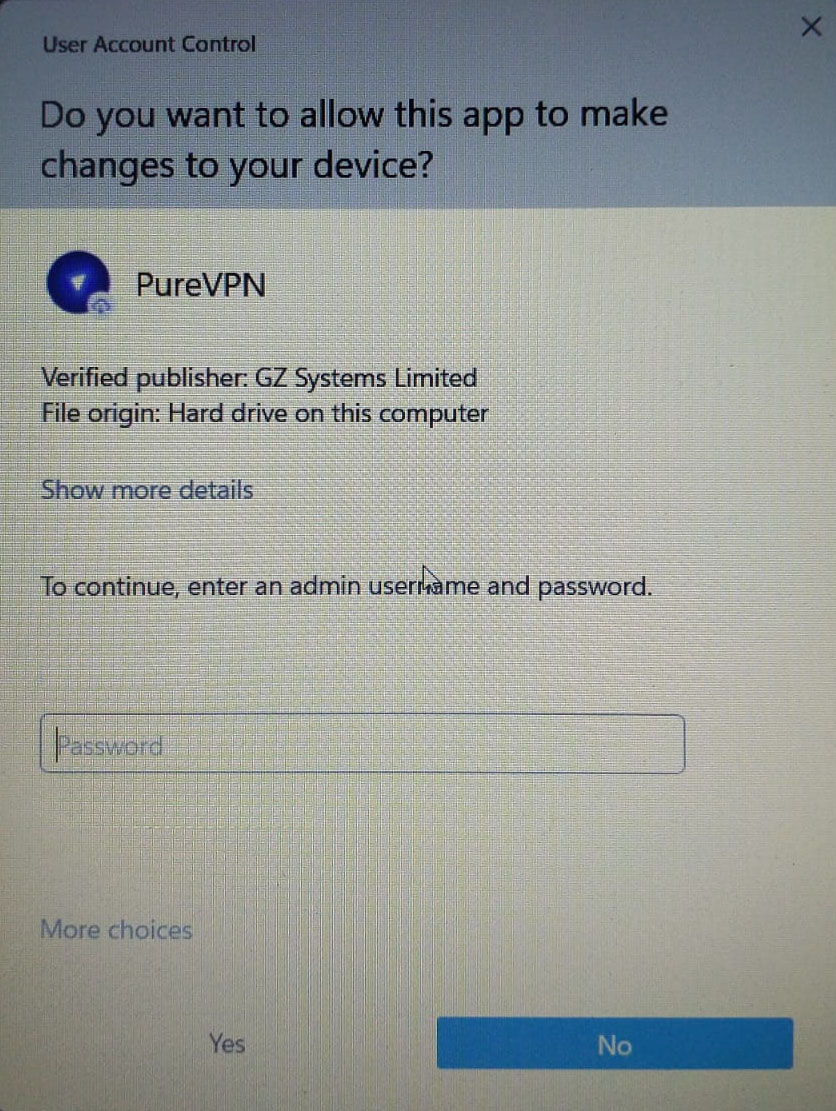
\includegraphics[width=10cm]{3.png}
\centering
\caption{Окно с разрешением}
\label{fig:3}
\end{figure}
\item PureVPN готов к установке.
\item Чтобы начать установку, пожалуйста, ознакомьтесь с правилами и условиями.

После прочтения правил и условий отметьте галочкой, затем нажмите Далее , чтобы продолжить:  Рисунок(\ref{fig:4})
\begin{figure}[H]
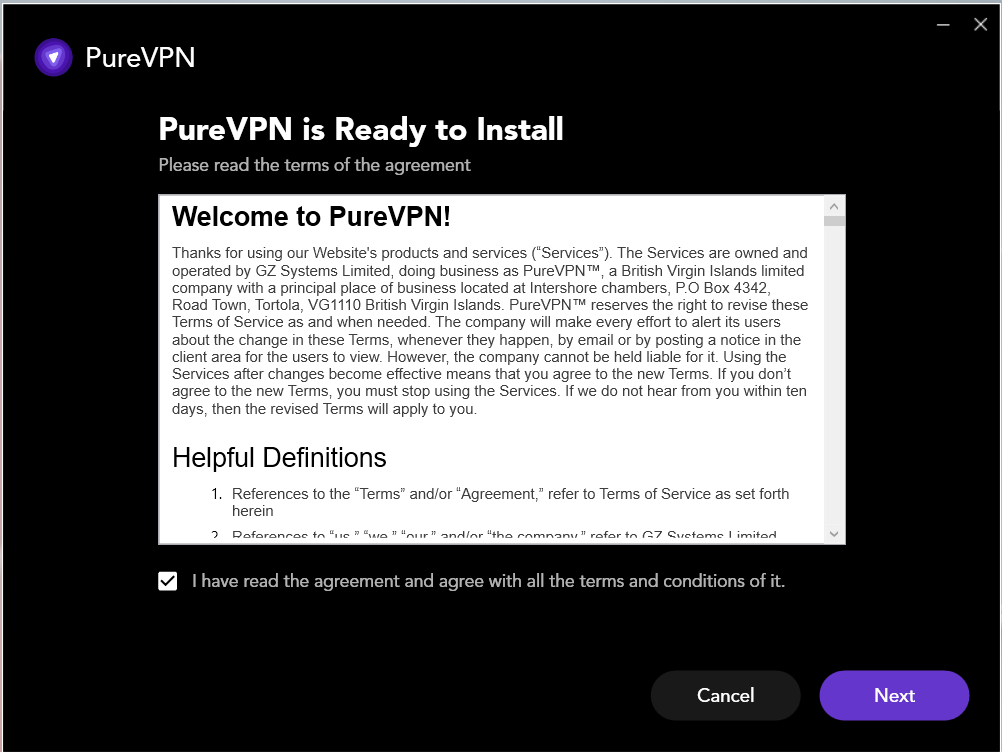
\includegraphics[width=14cm]{4.png}
\centering
\caption{Правила и условия}
\label{fig:4}
\end{figure}
\item Подождите несколько секунд, и приложение запустится автоматически:  Рисунок(\ref{fig:5})
\begin{figure}[H]
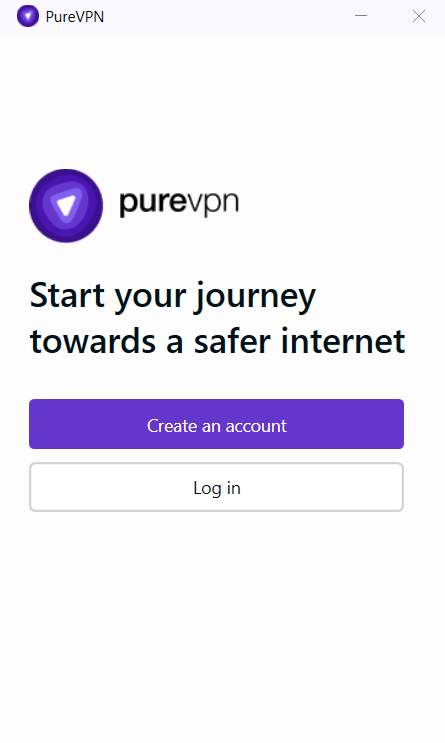
\includegraphics[width=8cm]{5.png}
\centering
\caption{Приложение}
\label{fig:5}
\end{figure}
\end{itemize}

\subsection{Войдите в приложение PureVPN} 
Как только ваша установка пройдет успешно. Вот как вы можете выполнить вход в приложение PureVPN.
\begin{itemize}
\item Запустите приложение PureVPN .
\item Нажмите на Вход:  Рисунок(\ref{fig:6})
\begin{figure}[H]
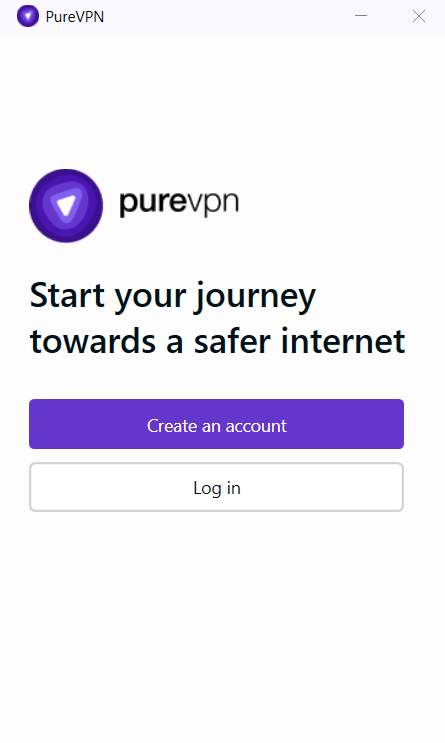
\includegraphics[width=8cm]{5.png}
\centering
\caption{Вход}
\label{fig:6}
\end{figure}
\item Появится всплывающее окно, в котором вам необходимо будет ввести свои учетные данные PureVPN.
\item Введите свой адрес электронной почты PureVPN и пароль (используйте адрес электронной почты и пароль, которые вы настроили при покупке).
\item После ввода данных учетной записи нажмите Войти:  Рисунок(\ref{fig:7})
\begin{figure}[H]
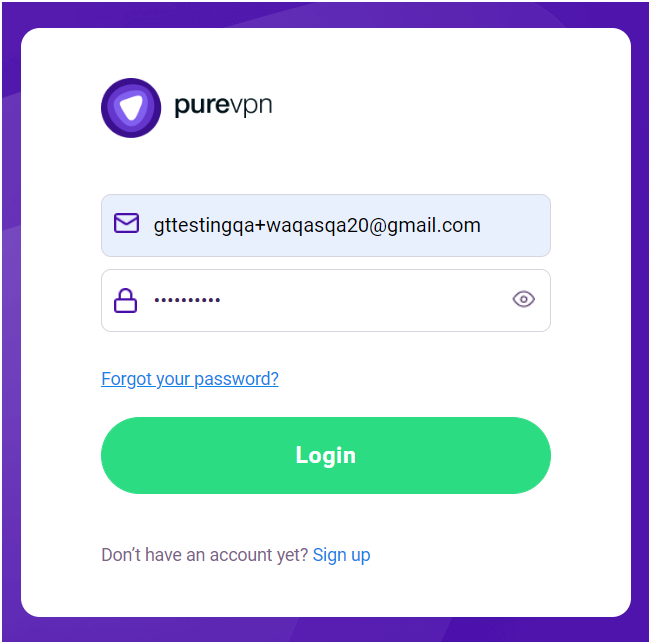
\includegraphics[width=10cm]{7.png}
\centering
\caption{Войти}
\label{fig:7}
\end{figure}
\item Выберите назначение, которое наилучшим образом соответствует вашим потребностям в VPN:  Рисунок(\ref{fig:8})
\begin{figure}[H]
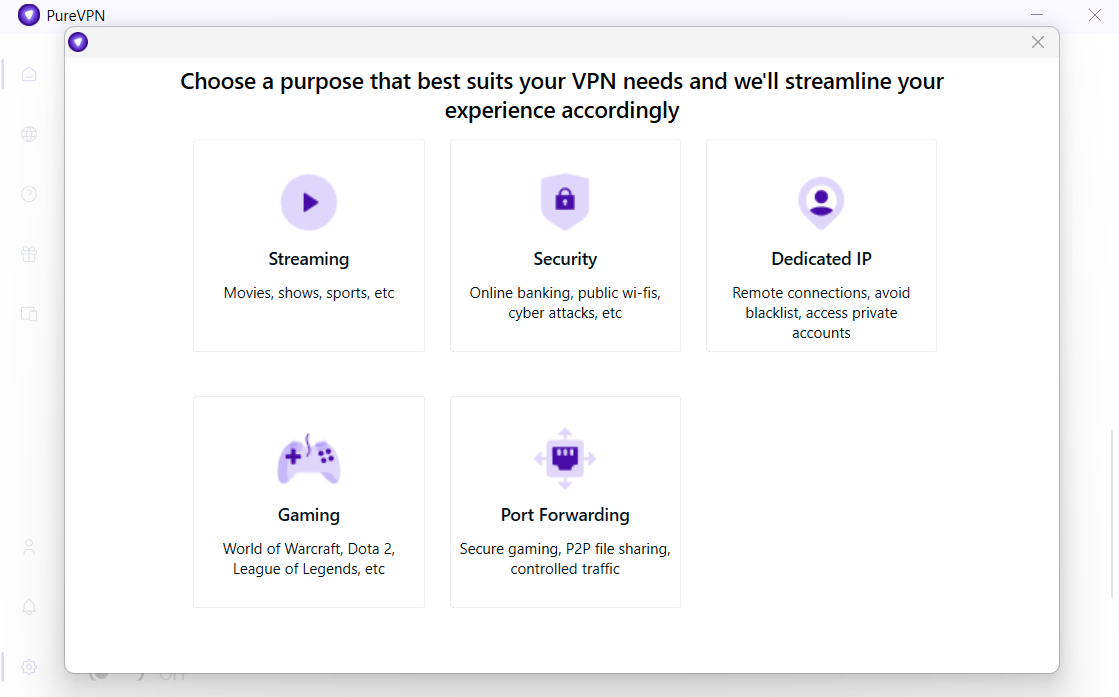
\includegraphics[width=14cm]{8.png}
\centering
\caption{Потребности}
\label{fig:8}
\end{figure}
\item Автоматически появится приложение PureVPN, и вы войдете в это приложение:  Рисунок(\ref{fig:9})
\begin{figure}[H]
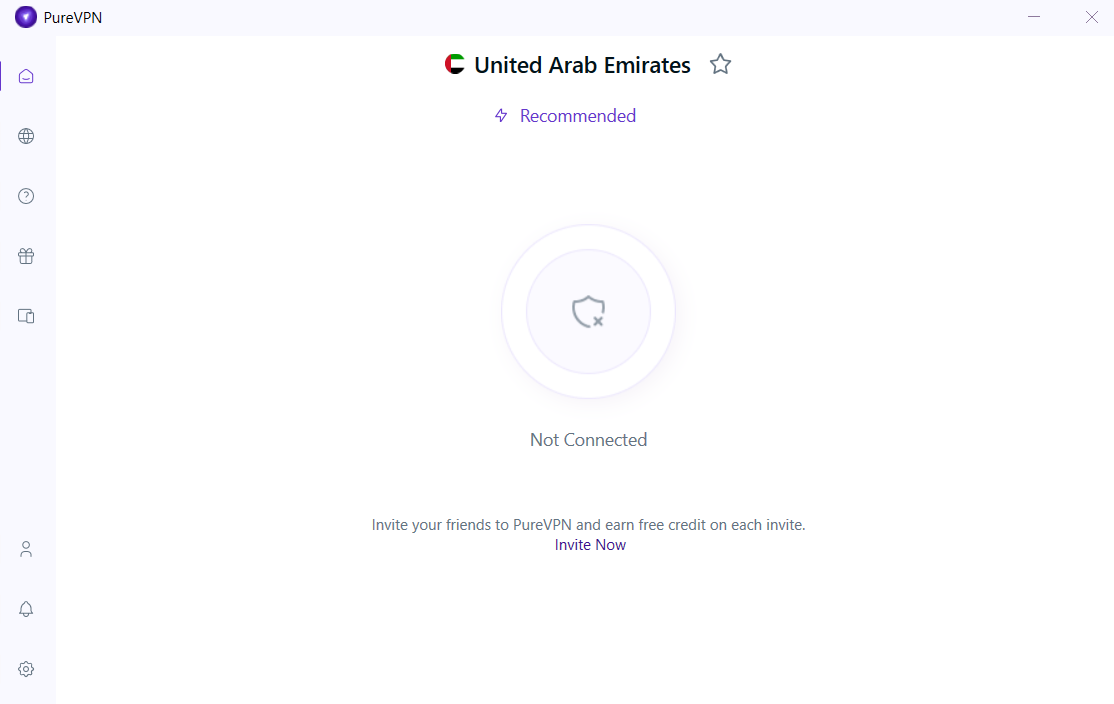
\includegraphics[width=14cm]{9.png}
\centering
\caption{Главная страница приложения}
\label{fig:9}
\end{figure}

Примечание:

Вам будет предложено выбрать учетную запись, если у вас есть несколько подписок на ваш электронный адрес PureVPN:  Рисунок(\ref{fig:10})
\begin{figure}[H]
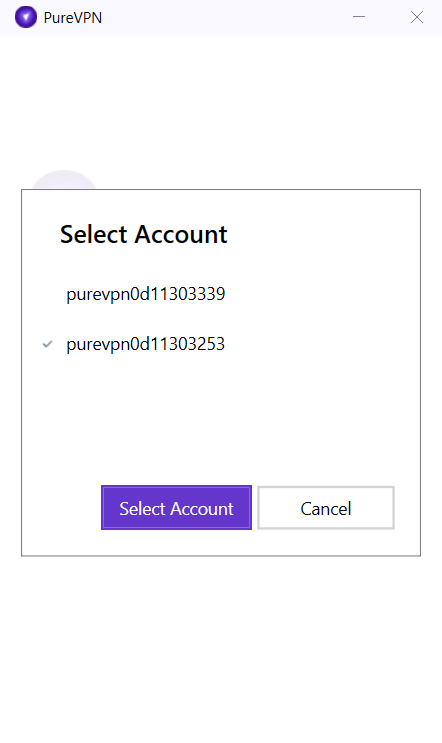
\includegraphics[width=8cm]{10.png}
\centering
\caption{Выбор учетной записи}
\label{fig:10}
\end{figure}
\item Теперь вы вошли в приложение PureVPN:  Рисунок(\ref{fig:11})
\begin{figure}[H]
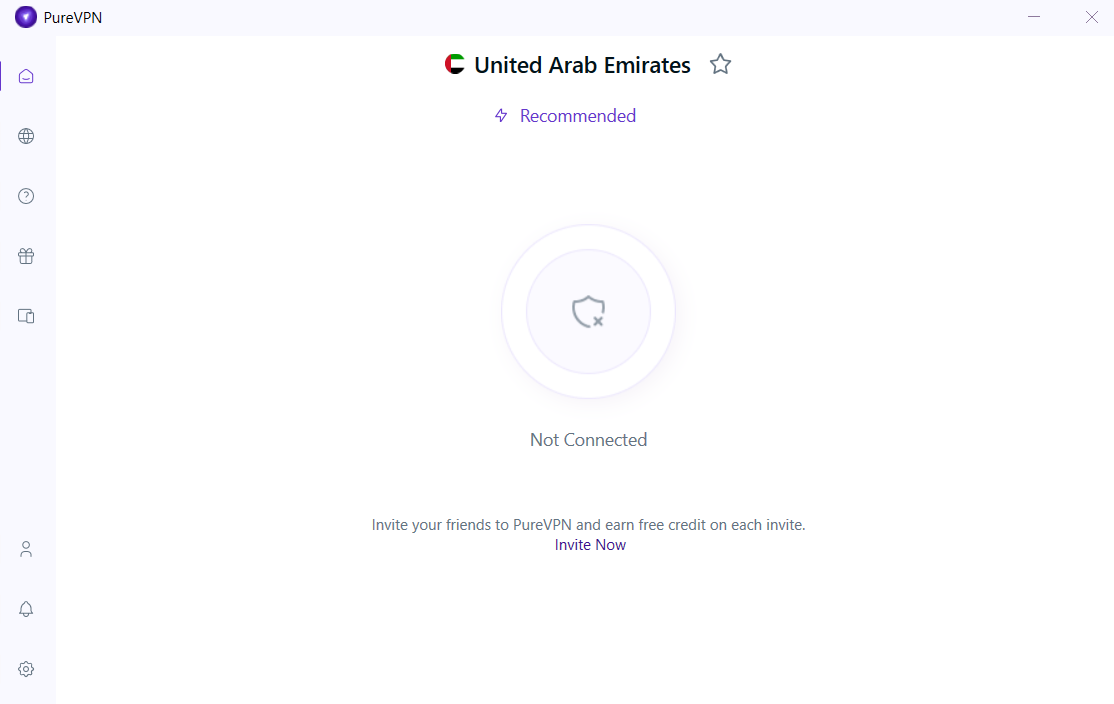
\includegraphics[width=12cm]{9.png}
\centering
\caption{Вы вошли в приложение PureVPN}
\label{fig:11}
\end{figure}
\end{itemize}

\subsection{Выход из приложения PureVPN для Windows} 
Хотите выйти из приложения PureVPN? Нет проблем ..!! Выполните простые шаги, приведенные ниже.
\begin{itemize}
\item Щелкните по значку пользователя на левой панели приложения PureVPN:  Рисунок(\ref{fig:12})
\begin{figure}[H]
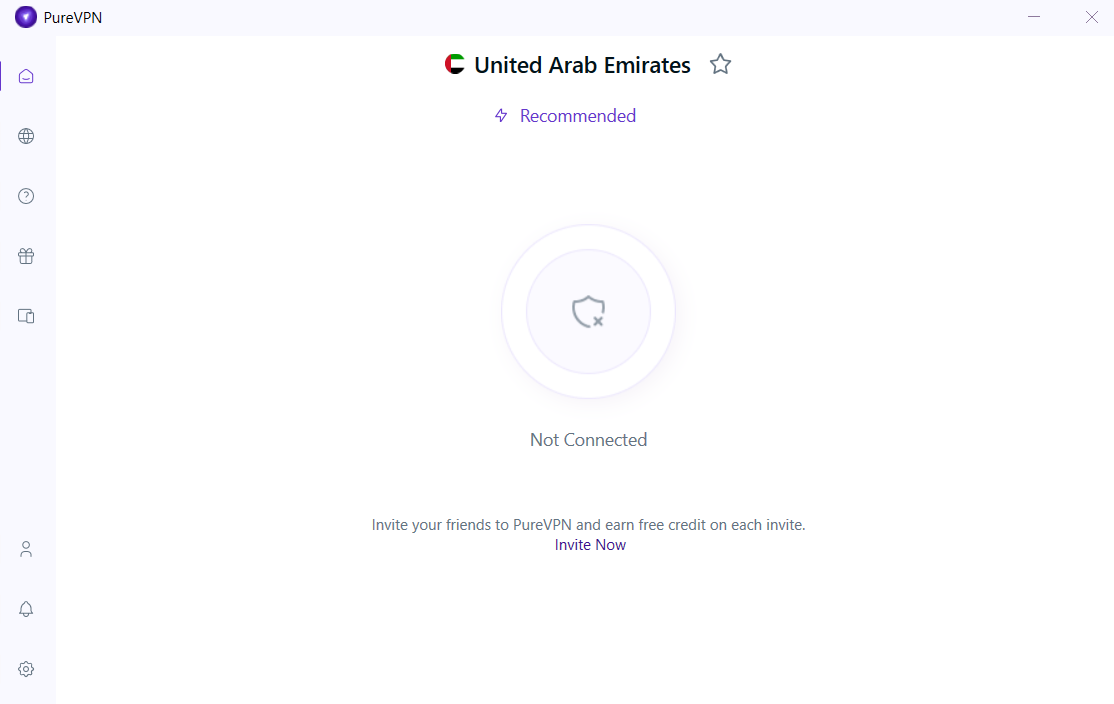
\includegraphics[width=12cm]{9.png}
\centering
\caption{Главная страница приложения}
\label{fig:12}
\end{figure}
\item Нажмите Выход из системы:  Рисунок(\ref{fig:13})
\begin{figure}[H]
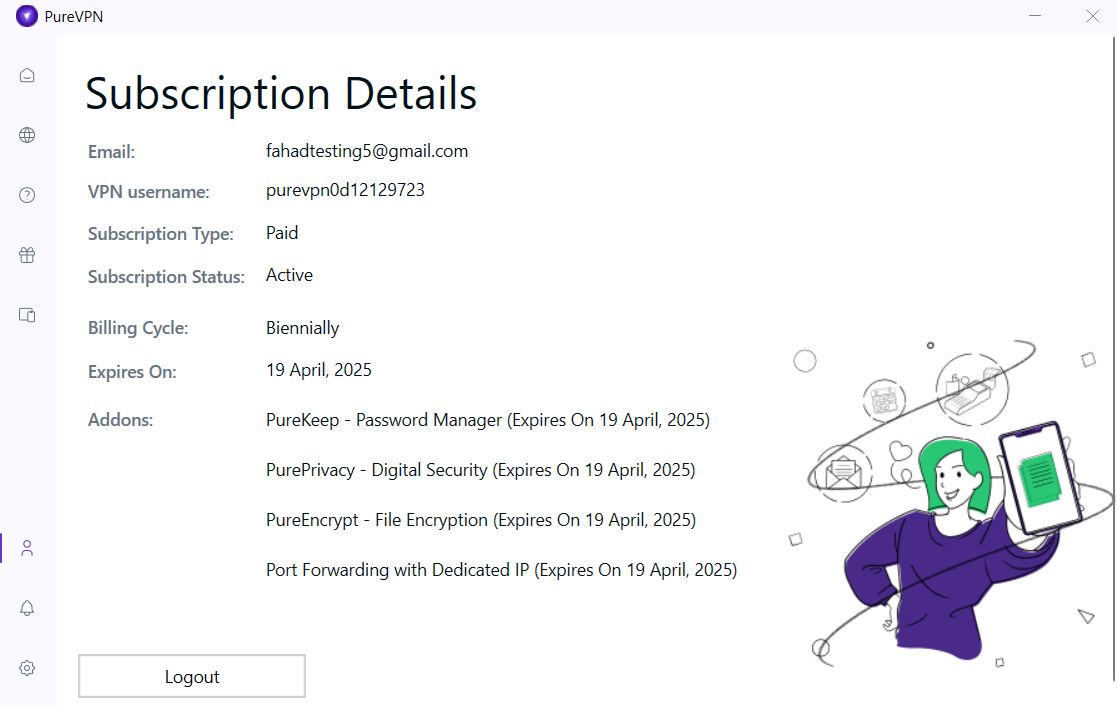
\includegraphics[width=12cm]{11.png}
\centering
\caption{Выход из системы}
\label{fig:13}
\end{figure}
\item Нажмите Да для подтверждения и продолжения:  Рисунок(\ref{fig:14})
\begin{figure}[H]
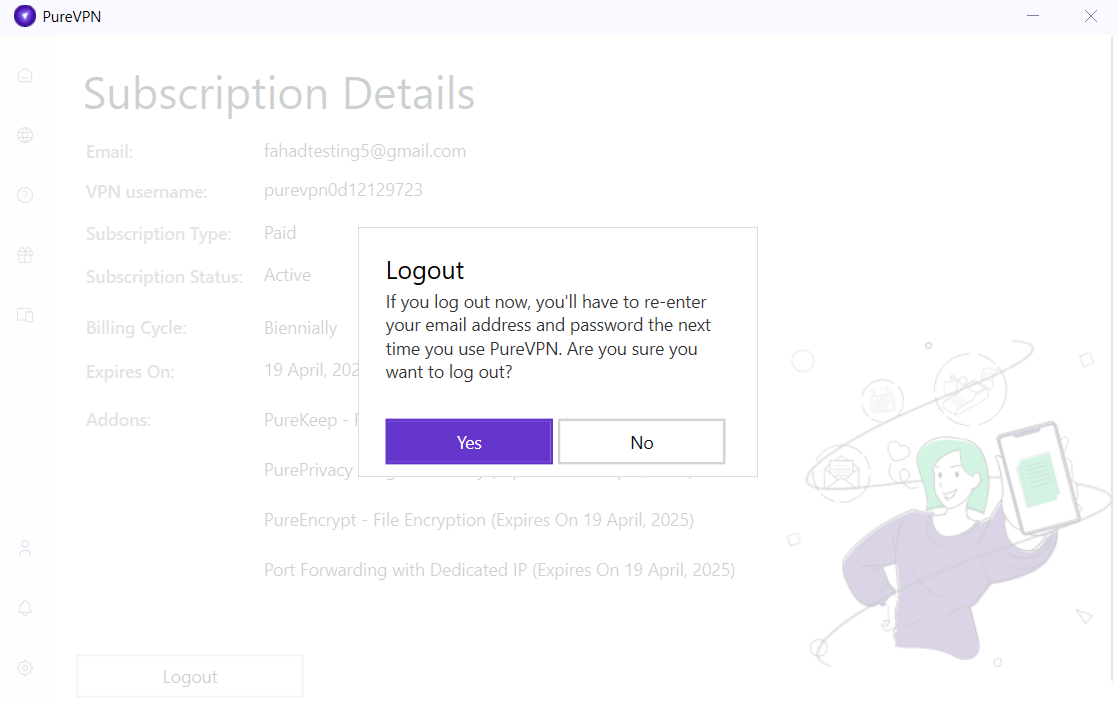
\includegraphics[width=12cm]{12.png}
\centering
\caption{Окно подтверждение действия}
\label{fig:14}
\end{figure}
\item Вы успешно вышли из приложения PureVPN:  Рисунок(\ref{fig:15})
\begin{figure}[H]
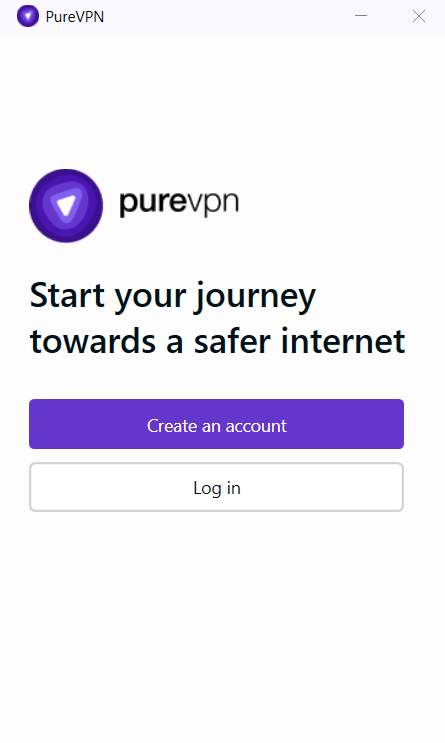
\includegraphics[width=8cm]{5.png}
\centering
\caption{Успешный выход из приложения}
\label{fig:15}
\end{figure}
\end{itemize}

\subsection{Проверьте сведения о подписке в приложении PureVPN} 
Ищете способ просмотреть сведения о вашей подписке в приложении PureVPN? Следуйте приведенным ниже инструкциям, чтобы иметь возможность просматривать сведения о вашей подписке в приложении PureVPN.
\begin{itemize}
\item Щелкните по значку пользователя на левой панели приложения PureVPN:  Рисунок(\ref{fig:16})
\begin{figure}[H]
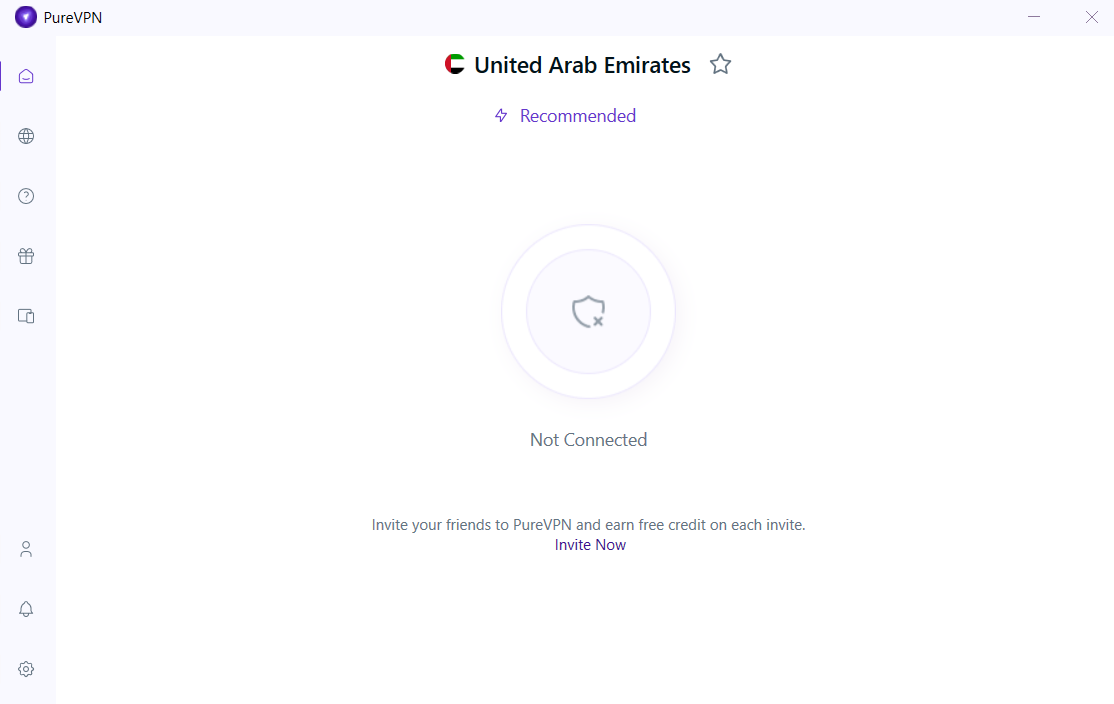
\includegraphics[width=12cm]{9.png}
\centering
\caption{Главная страница приложения}
\label{fig:16}
\end{figure}
\item В разделе профиля вы сможете просмотреть сведения о подписке.
\item Ниже приведены сведения, которые будут видны в разделе Профиля:  Рисунок(\ref{fig:17})
\begin{enumerate}
\item Электронная почта
\item Имя пользователя VPN
\item Тип подписки
\item Статус подписки
\item Цикл выставления счетов
\item Срок действия подписки истек
\item Аддоны
\end{enumerate}
\begin{figure}[H]
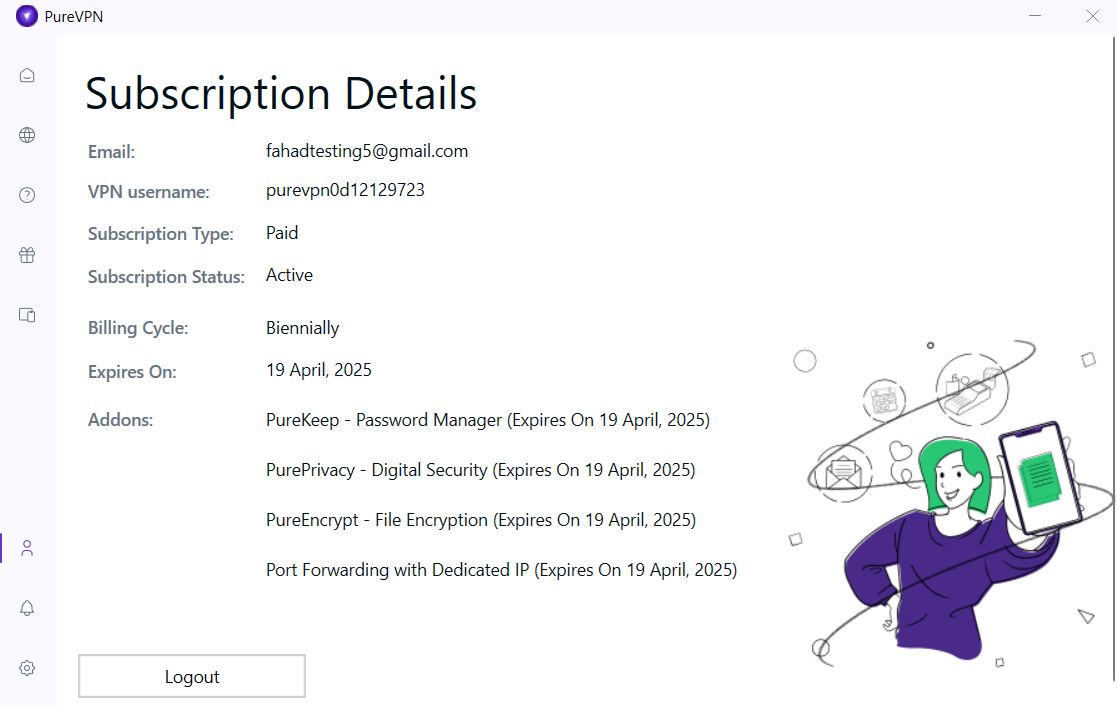
\includegraphics[width=12cm]{11.png}
\centering
\caption{Сведения о подписке}
\label{fig:17}
\end{figure}
\end{itemize}

\section{Linux}

\subsection{Подключите Wireguard в Linux} 
\begin{itemize}
\item Перейдите в окно терминала и введите следующие команды одну за другой, чтобы установить необходимые пакеты:
\begin{enumerate}
\item sudo bash
\item sudo apt-получить обновление
\item sudo apt-получить установку wireguard
\end{enumerate}

\item Выполните следующую команду, чтобы создать VPN-соединение Wireguard.

sudo nano /etc/wireguard/wg0.conf
\item Как только файл будет загружен, вам нужно будет загрузить файл конфигурации wireguard и нажать ‘Скопировать в буфер обмена’ (см. Шаги ниже, чтобы получить файл конфигурации Wireguard).
\item Следующий шаг - зайти в свой профиль vpn, вставить туда содержимое.
\item Нажмите Сохранить и закройте профиль:  Рисунок(\ref{fig:18})
\begin{figure}[H]
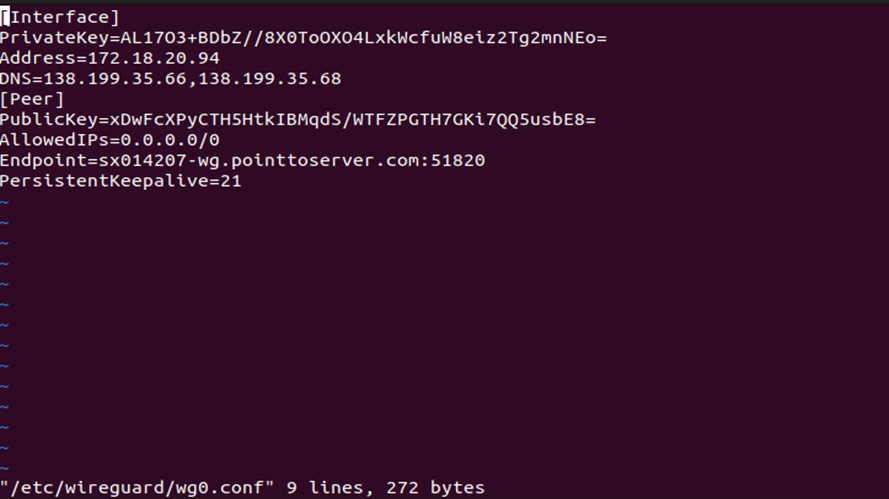
\includegraphics[width=12cm]{13.png}
\centering
\caption{Содержимое в профиле vpn}
\label{fig:18}
\end{figure}
\item Чтобы активировать VPN-соединение Wireguard, выполните следующую команду.

sudo wg-ускоренный запуск wg0
\item Чтобы отключить соединение Wireguard, вы можете перейти к выполнению следующей команды.

sudo wg-быстрое отключение wg0
\end{itemize}

\subsection{Загрузите файл конфигурации Wireguard} 
\begin{itemize}
\item Войдите в учетную запись в личном кабинете PureVPN:  Рисунок(\ref{fig:19})
\begin{figure}[H]
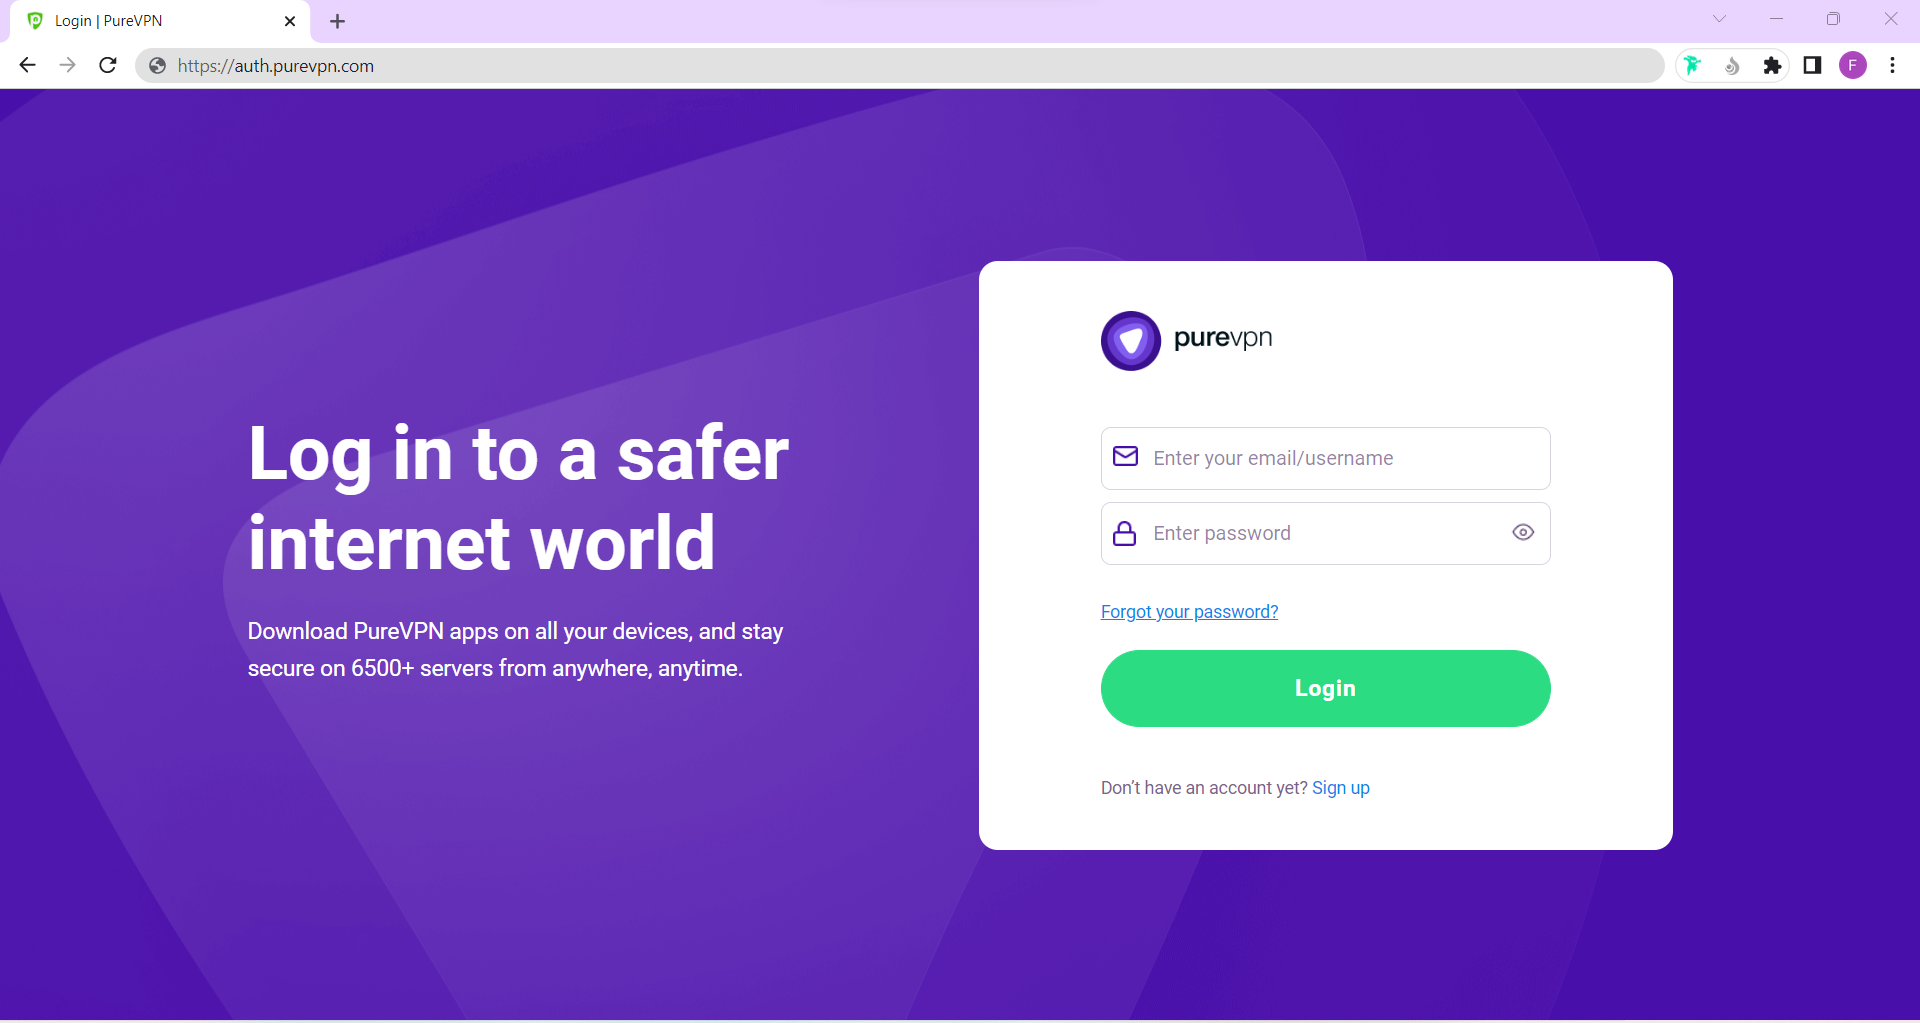
\includegraphics[width=12cm]{14.png}
\centering
\caption{Форма для входа в учетную запись}
\label{fig:19}
\end{figure}
\item Перейдите на вкладку Ручная настройка:  Рисунок(\ref{fig:20})
\begin{figure}[H]
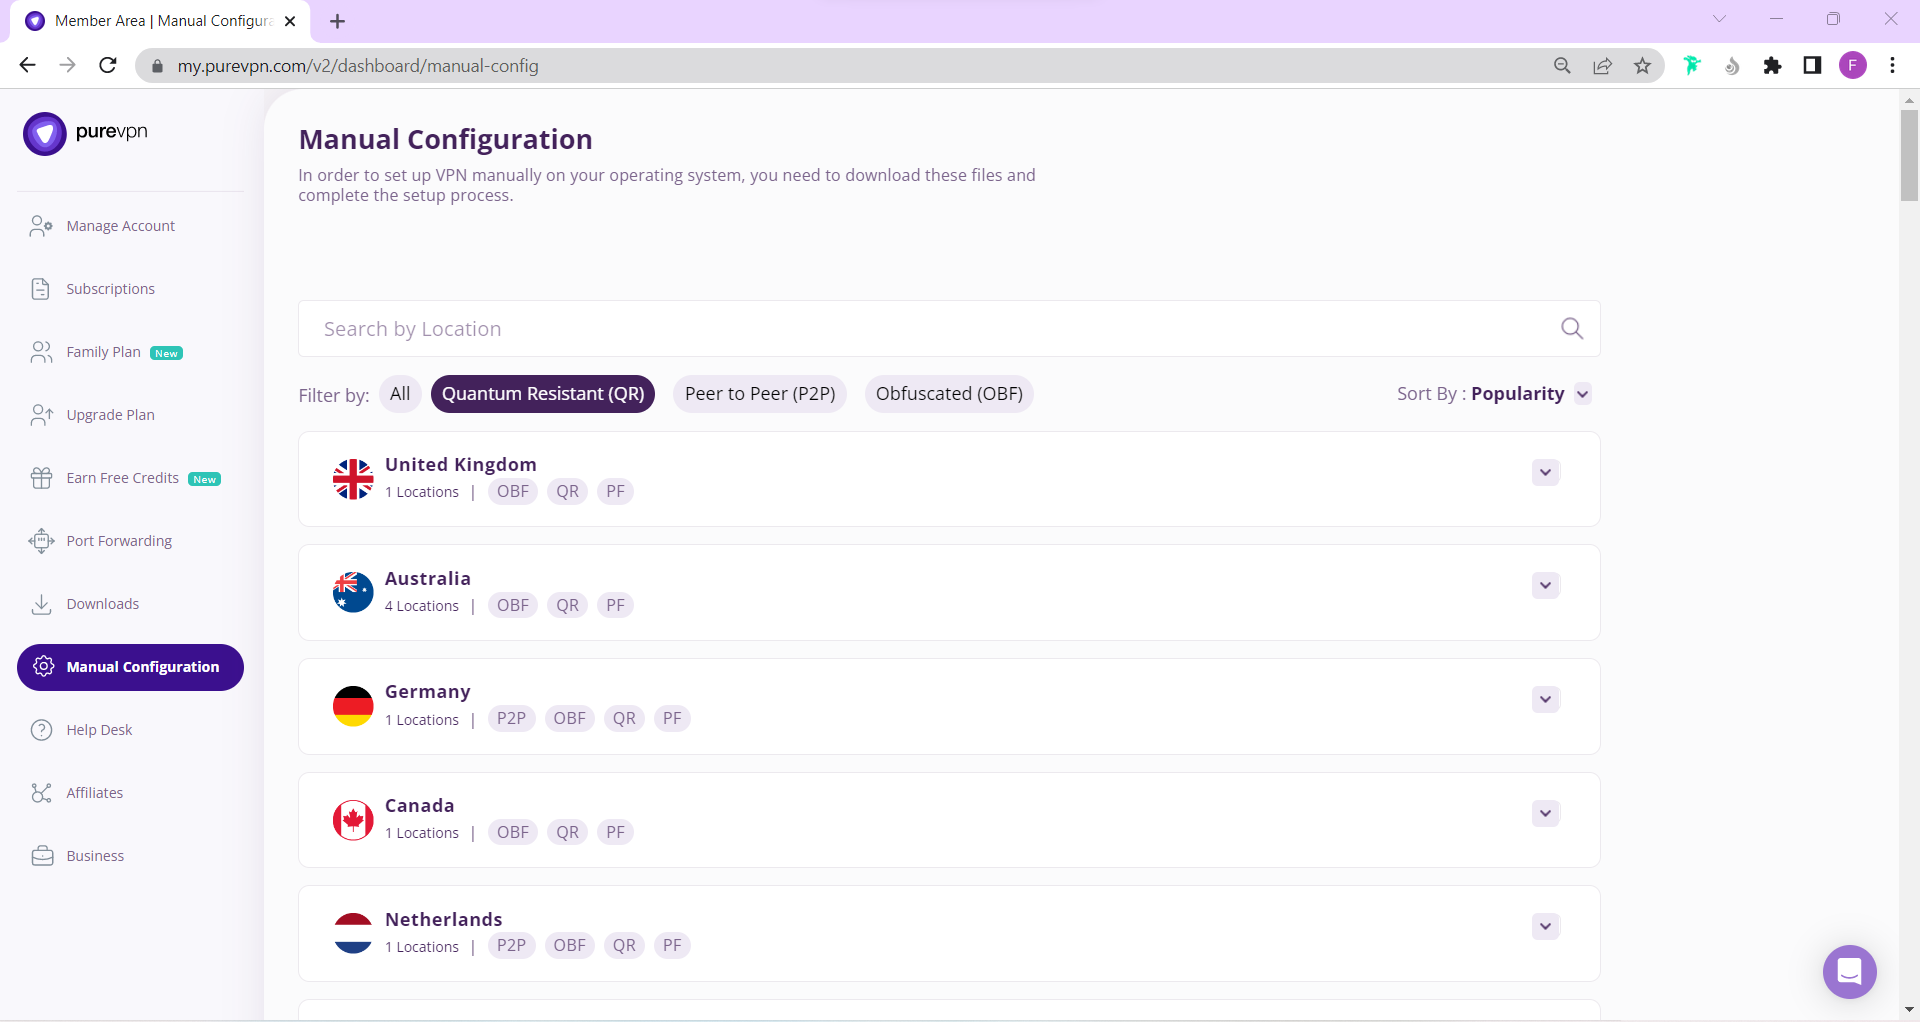
\includegraphics[width=12cm]{15.png}
\centering
\caption{Ручная настройка}
\label{fig:20}
\end{figure}
\item Нажмите на значок со стрелкой.
\item Выберите страну: к какому местоположению вы хотите подключиться?
\item Выберите город: к какому городу вы хотите подключиться из этой страны?
\item Нажмите кнопку Загрузить:  Рисунок(\ref{fig:21})
\begin{figure}[H]
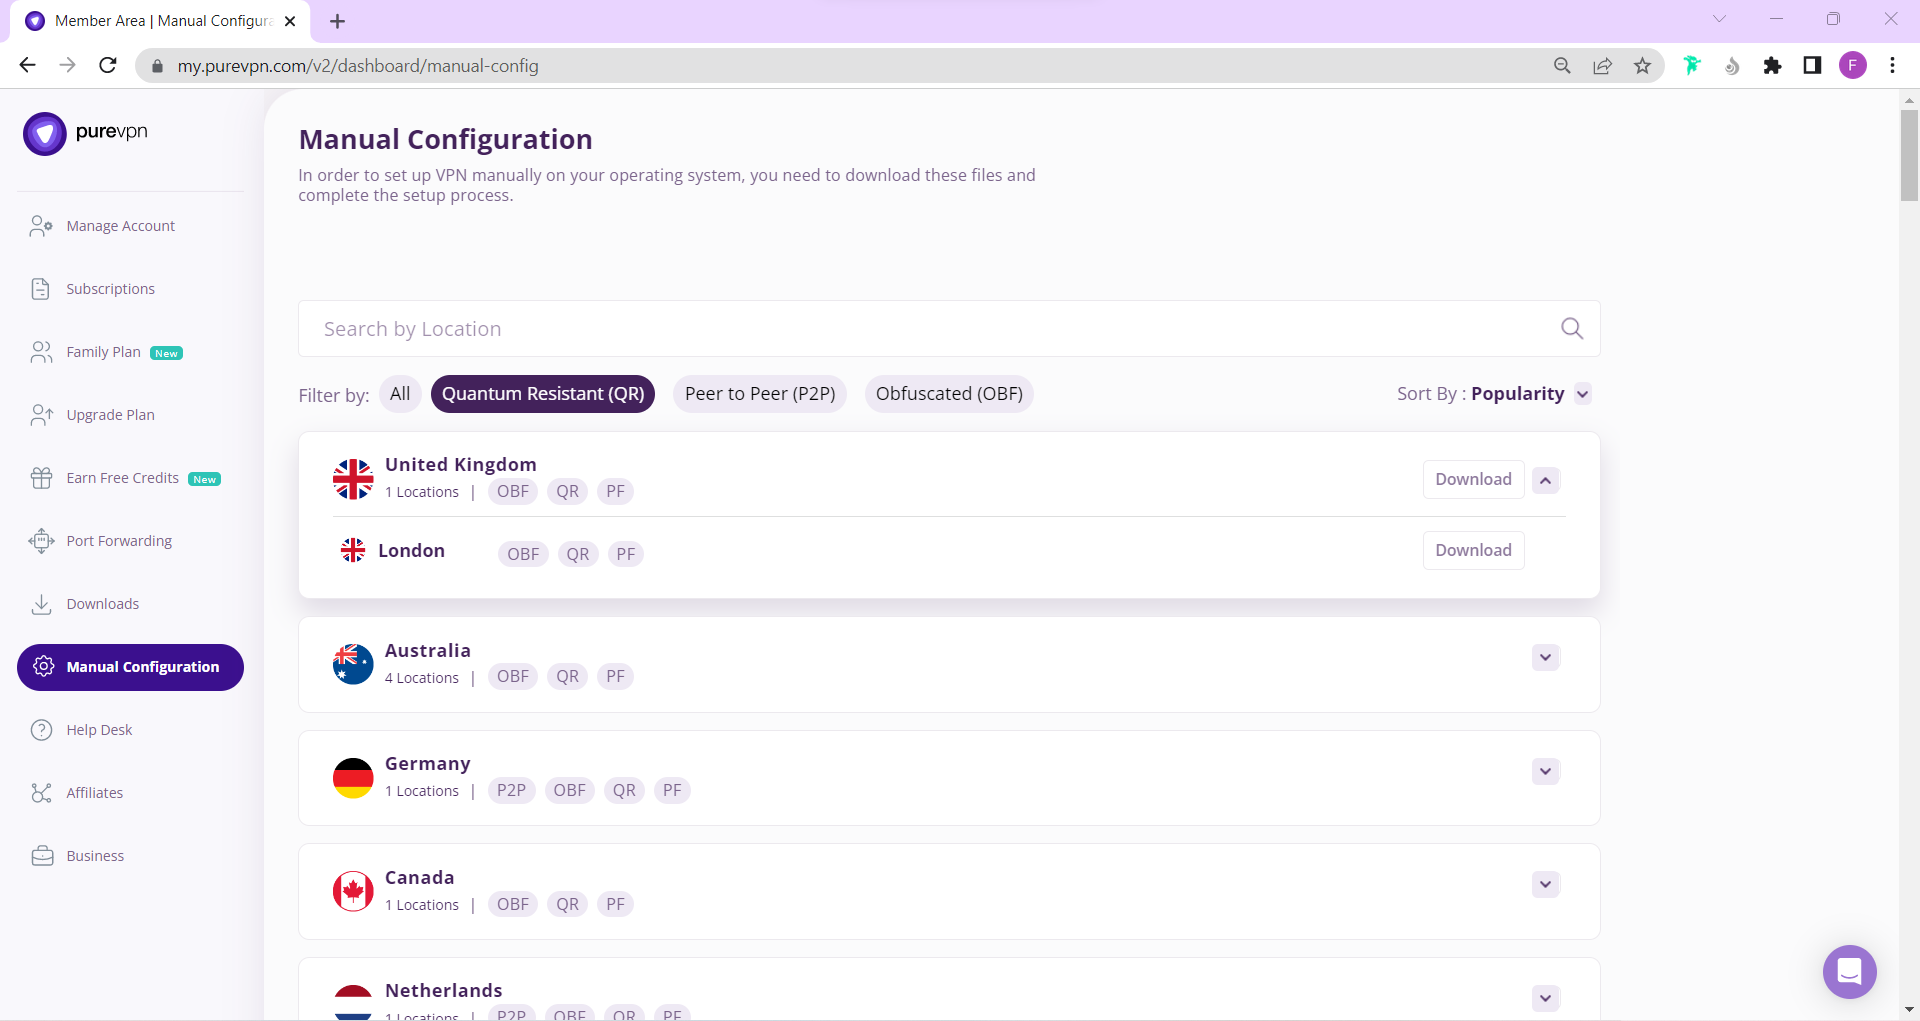
\includegraphics[width=12cm]{16.png}
\centering
\caption{Кнопка "Загрузить"}
\label{fig:21}
\end{figure}
\item Появится всплывающее окно с просьбой выбрать необходимую информацию.

Информация содержит следующее:  Рисунок(\ref{fig:22})
\begin{figure}[H]
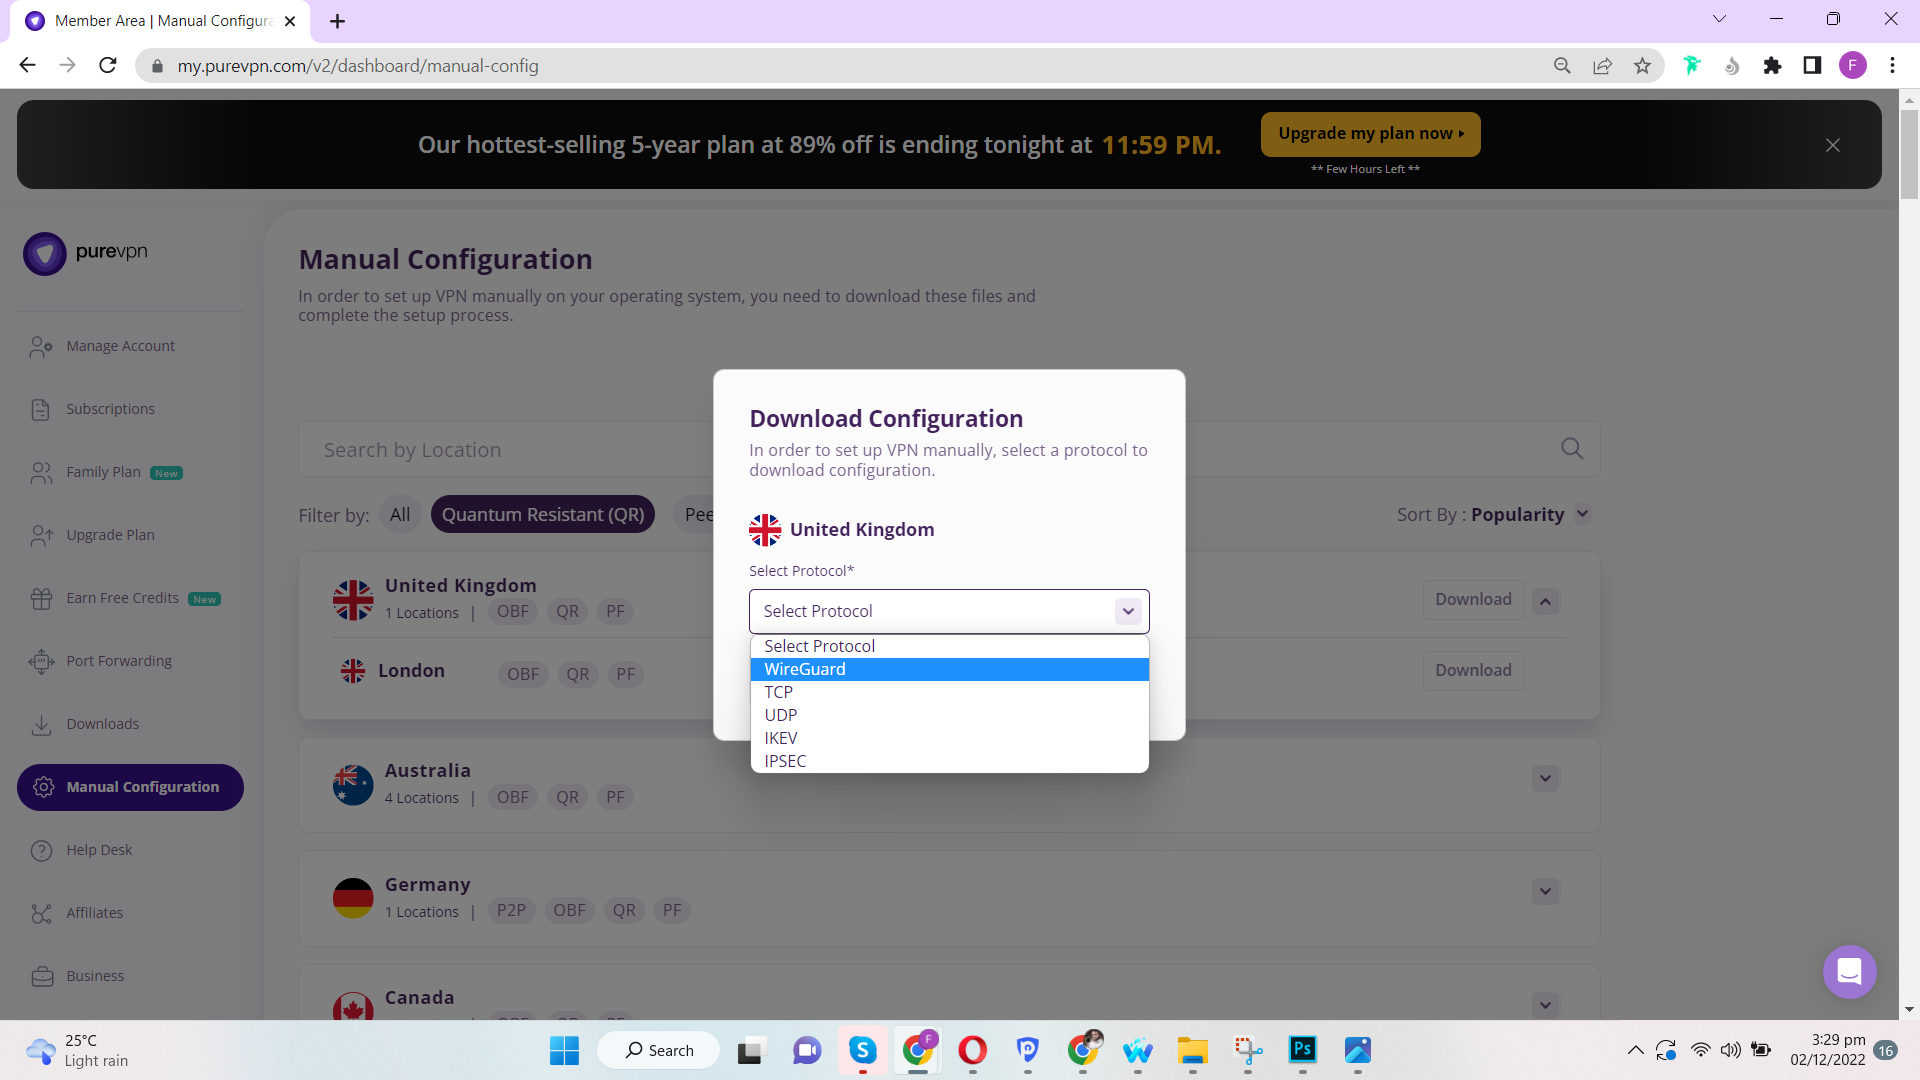
\includegraphics[width=12cm]{17.png}
\centering
\caption{Окно с информацией}
\label{fig:22}
\end{figure}
\item Выберите устройство: к какому устройству вы хотите подключиться? :  Рисунок(\ref{fig:23})
\begin{figure}[H]
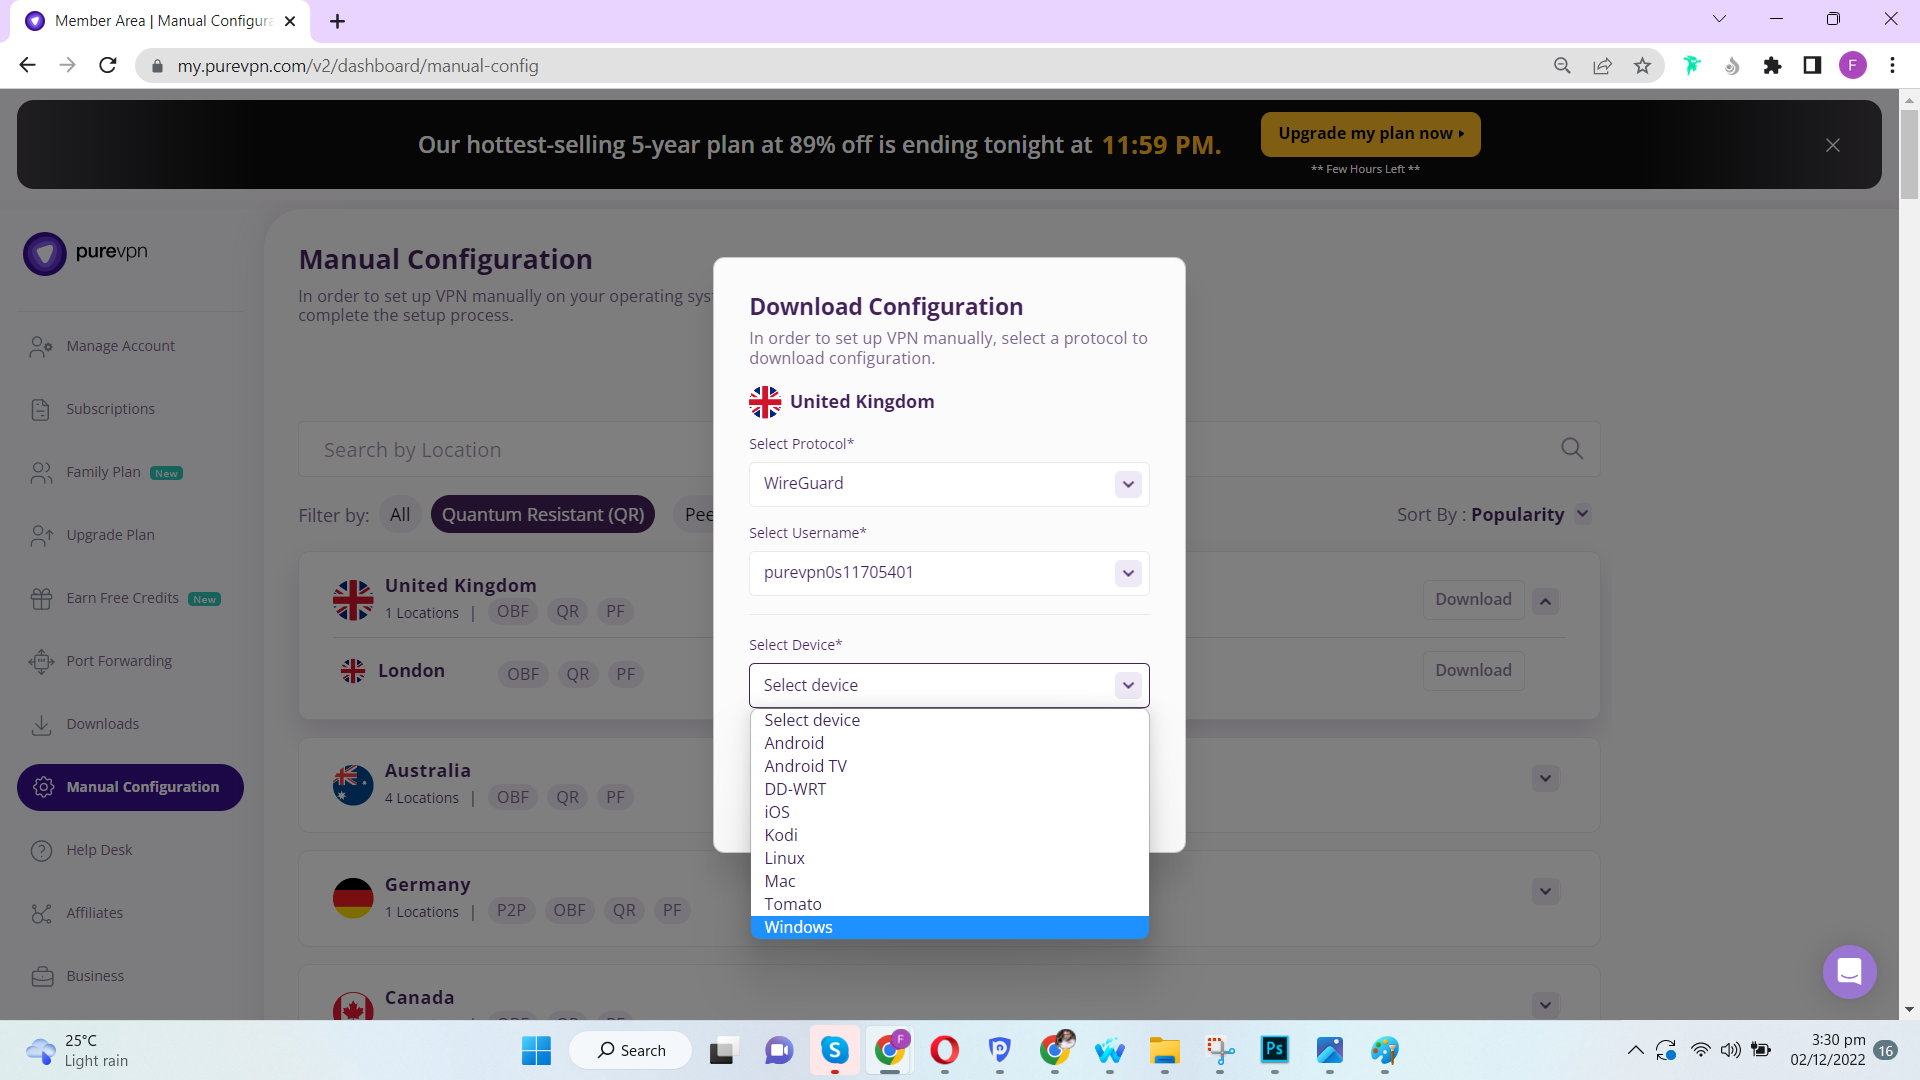
\includegraphics[width=12cm]{18.png}
\centering
\caption{Выбор устройства}
\label{fig:23}
\end{figure}
\item После ввода сведений вы сможете увидеть опцию копирования файла конфигурации:  Рисунок(\ref{fig:24})
\begin{figure}[H]
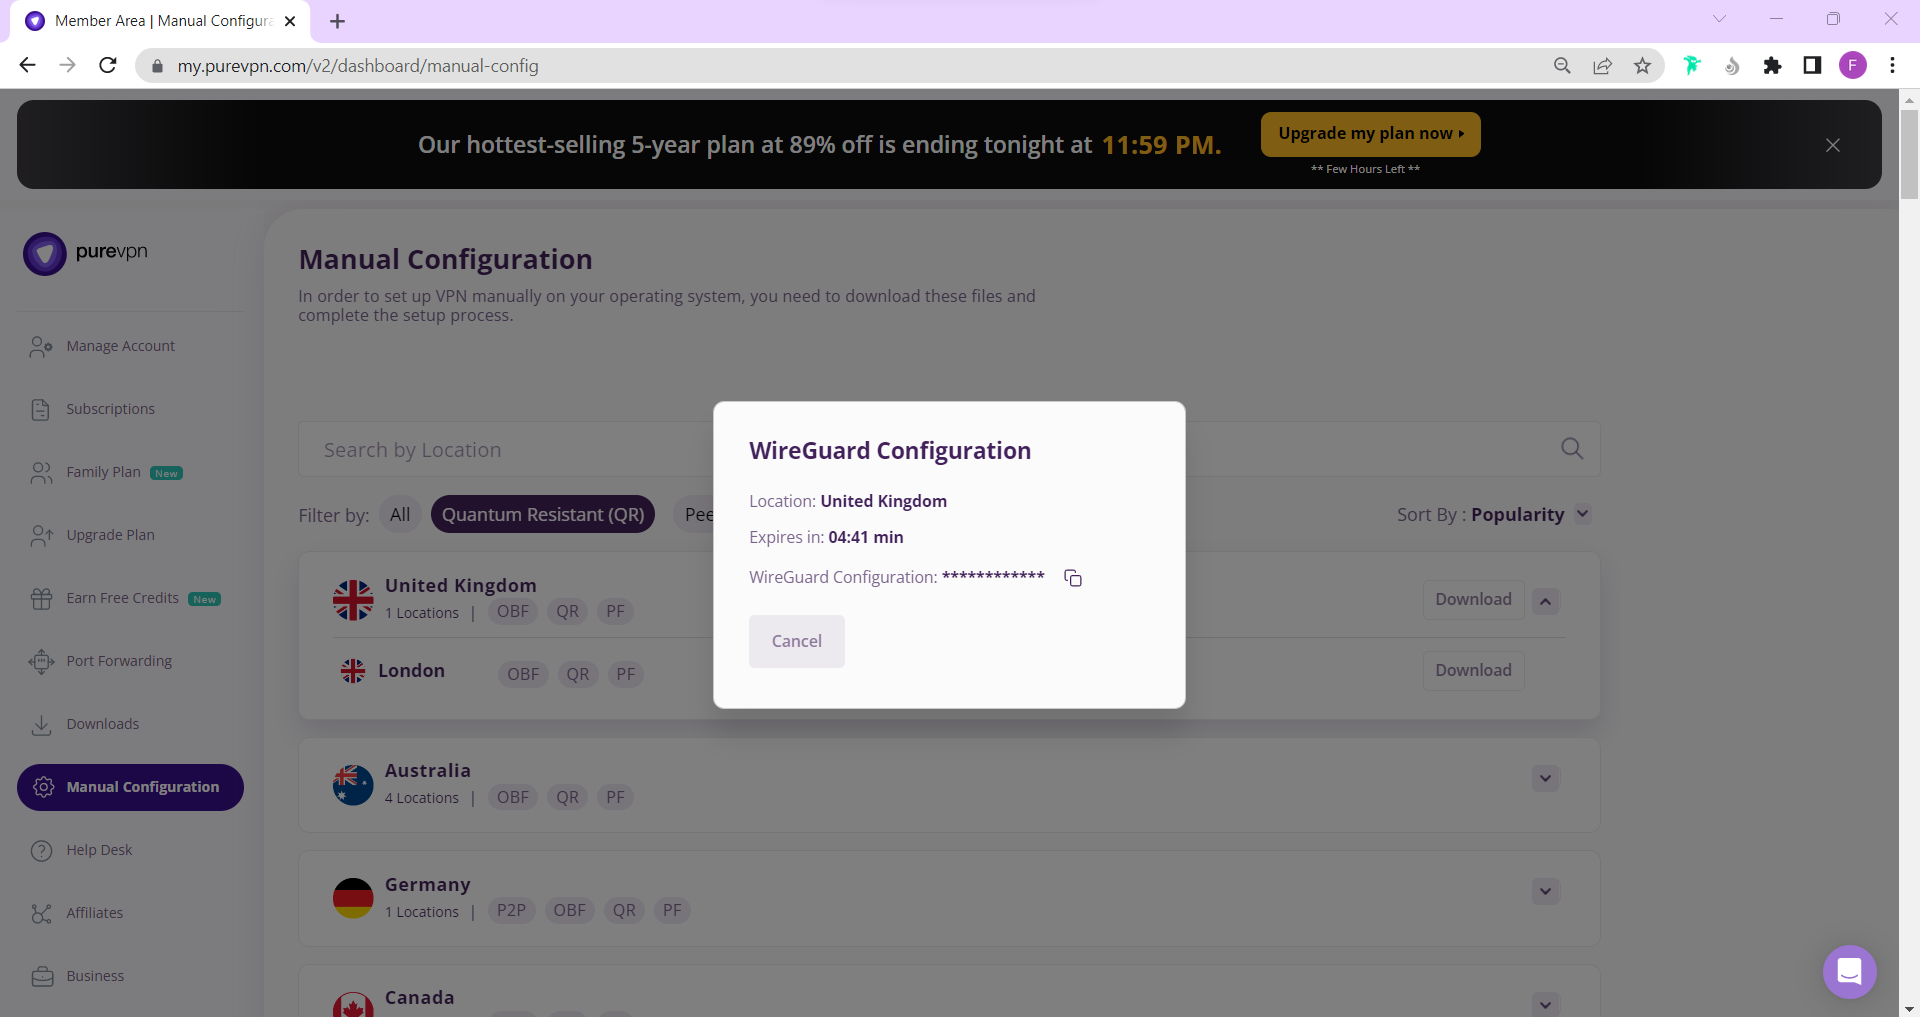
\includegraphics[width=12cm]{19.png}
\centering
\caption{Опция копирования файла конфигурации}
\label{fig:24}
\end{figure}

Примечание:

Пожалуйста, не забудьте скопировать файл и активировать соединение в течение 2 минут после загрузки профиля, в противном случае срок действия конфигурации истечет, и вам придется заново загружать новый файл конфигурации.
\end{itemize}

\section{Mac}

\subsection{Загрузите приложение PureVPN} 
\begin{itemize}
\item Перейдите по ссылке https://www.purevpn.com/download/windows-vpn, чтобы перейти на страницу загрузки приложения PureVPN.
\item Нажмите кнопку Загрузить приложение, чтобы загрузить приложение PureVPN на свое устройство:  Рисунок(\ref{fig:25})
\begin{figure}[H]
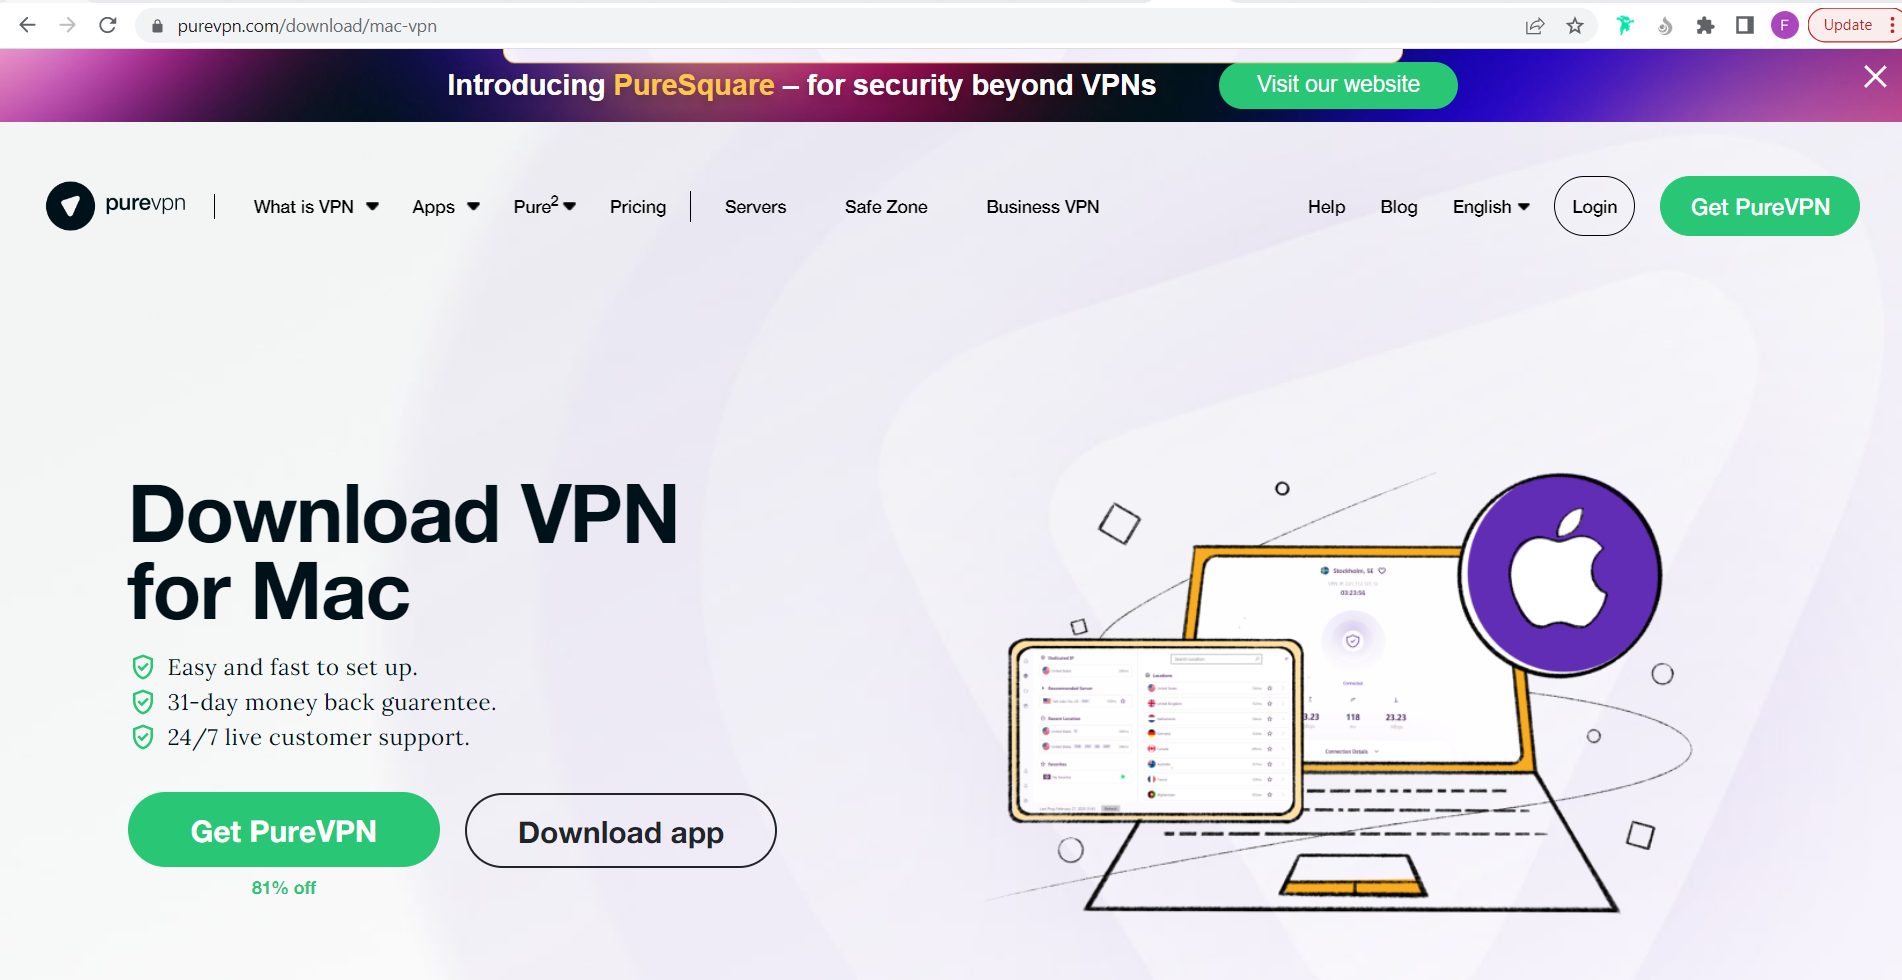
\includegraphics[width=14cm]{20.png}
\centering
\caption{Загрузить приложение}
\label{fig:25}
\end{figure}
\item После завершения загрузки найдите установочный файл на своем устройстве. Скорее всего, вы найдете его в папке Downloads вашего устройства.
\end{itemize}

\subsection{Установите приложение PureVPN} 
Если вы ищете простой способ установить приложение PureVPN на свой macOS, вы можете воспользоваться нашим простым в использовании руководством здесь. Руководство проведет вас через весь процесс установки от начала до конца.
\begin{itemize}
\item Дважды щелкните, чтобы запустить программу установки PureVPN app:  Рисунок(\ref{fig:26})
\begin{figure}[H]
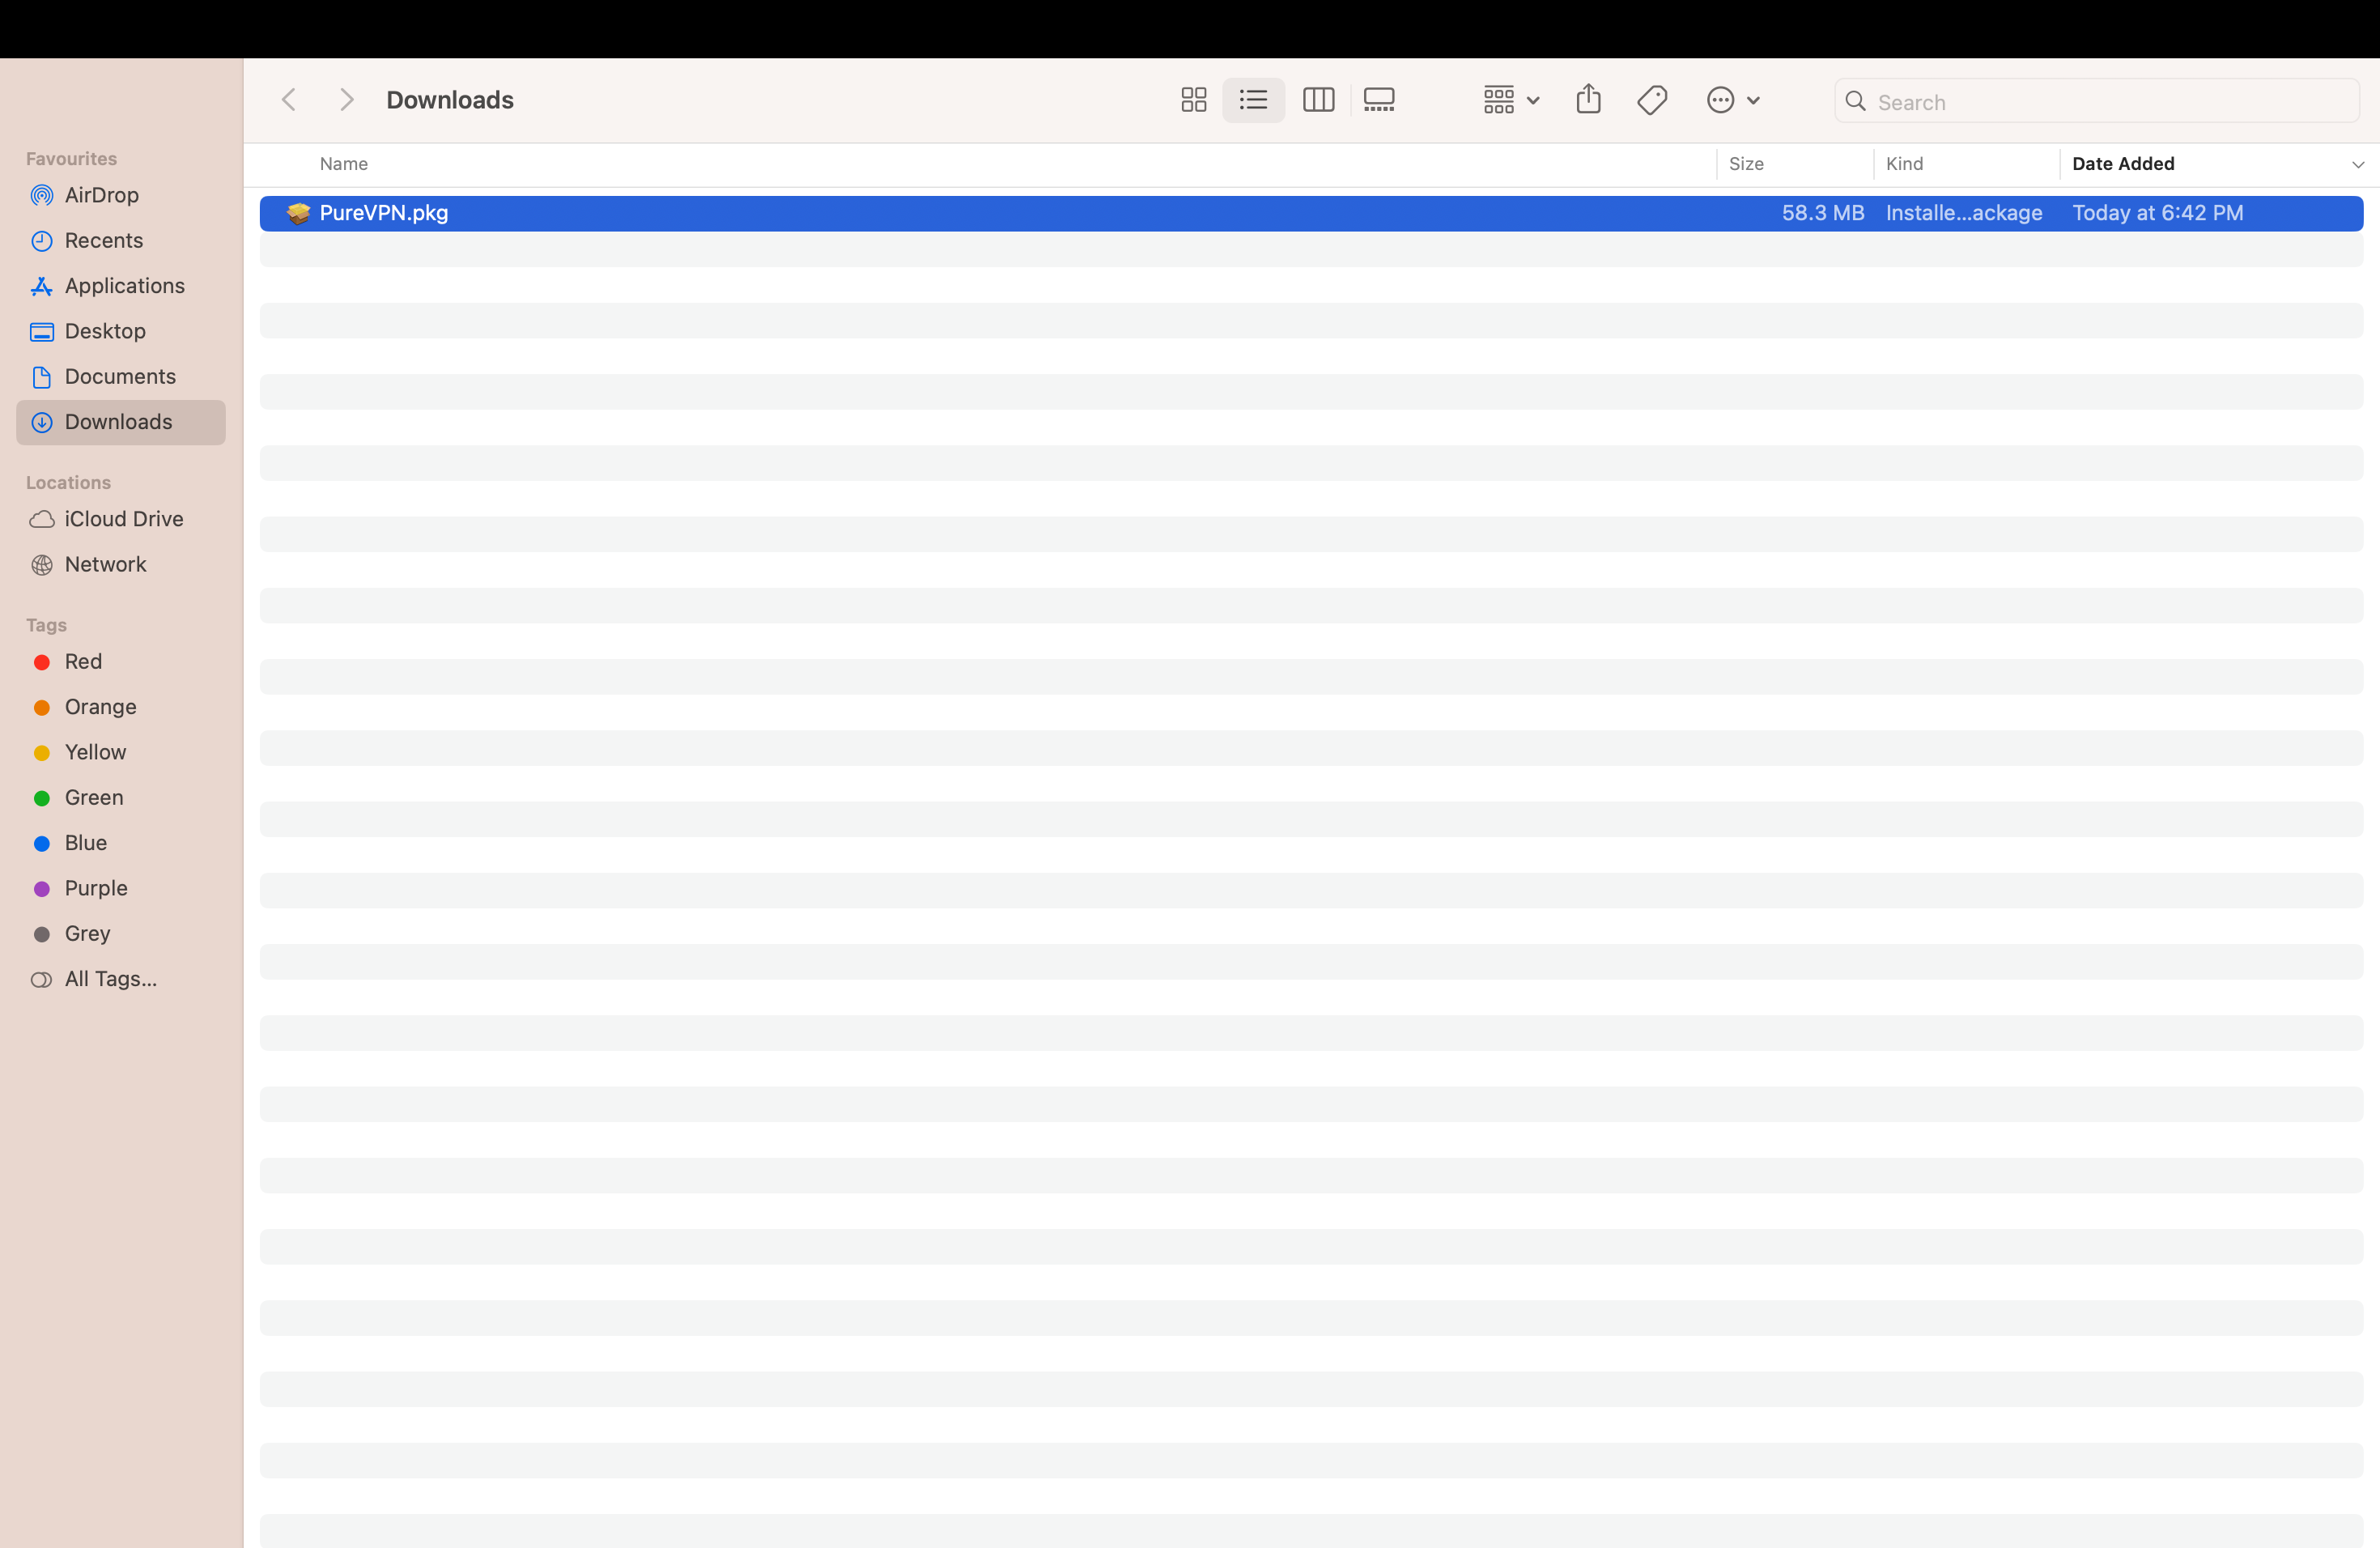
\includegraphics[width=14cm]{21.png}
\centering
\caption{ PureVPN app}
\label{fig:26}
\end{figure}
\item Для установки приложения PureVPN вам потребуется достаточно места в папке назначения:  Рисунок(\ref{fig:27})
\begin{figure}[H]
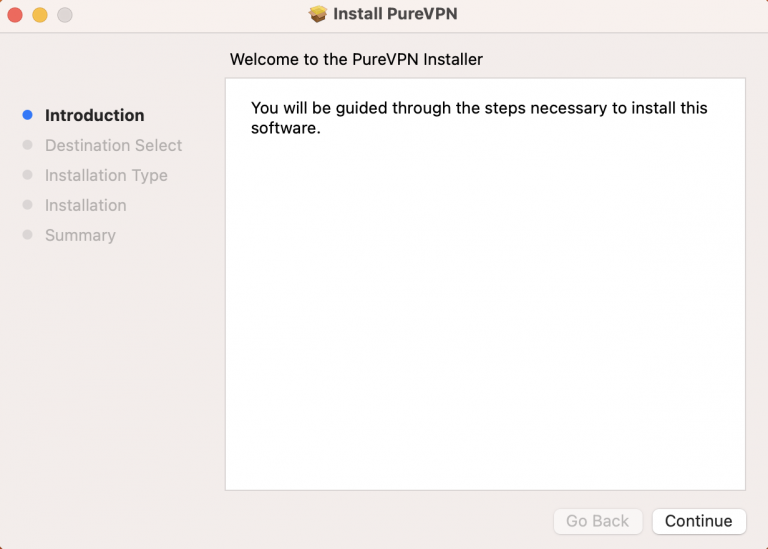
\includegraphics[width=14cm]{22.png}
\centering
\caption{Окно запроса}
\label{fig:27}
\end{figure}

Появится окно запроса с просьбой ввести имя пользователя и пароль для macOS.
\item После ввода имени пользователя и пароля macOS нажмите кнопку Установить программное обеспечение.
\item После завершения установки вы можете продолжить закрывать окно установки:  Рисунок(\ref{fig:28})
\begin{figure}[H]
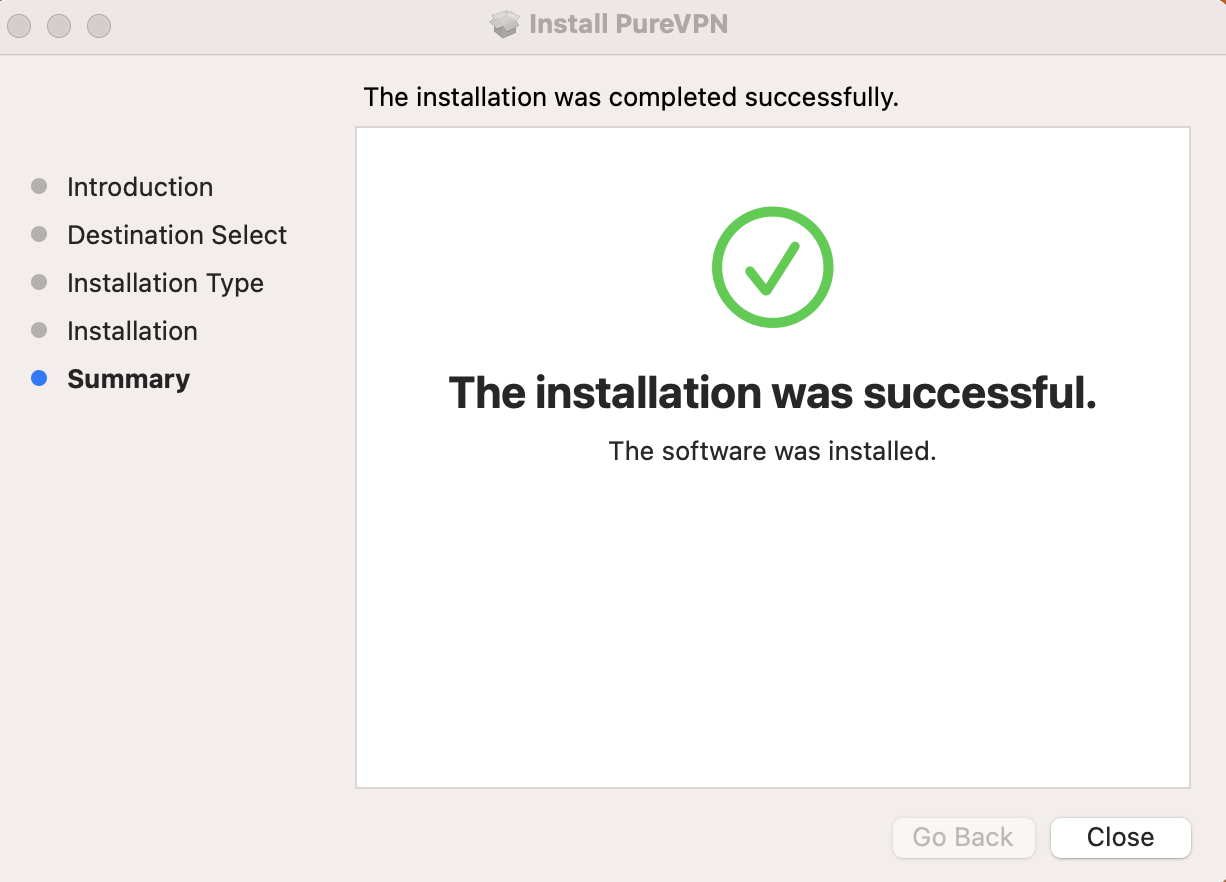
\includegraphics[width=14cm]{23.png}
\centering
\caption{Окно запроса}
\label{fig:28}
\end{figure}
\end{itemize}

Если вам не удается установить приложение PureVPN, вы можете выполнить следующие действия: Откройте меню Apple> Системные настройки> Безопасность и конфиденциальность> вкладку Общие. В разделе Разрешить приложения, загруженные из App Store, выберите App Store и идентифицированных разработчиков:

\subsection{Войдите в приложение PureVPN} 
Как только приложение установлено, вы можете приступить к запуску приложения и войти в него.

Как только ваша установка пройдет успешно. Вот как вы можете выполнить вход в приложение PureVPN.
\begin{itemize}
\item Запустите приложение PureVPN .
\item Нажмите Войти:  Рисунок(\ref{fig:29})
\begin{figure}[H]
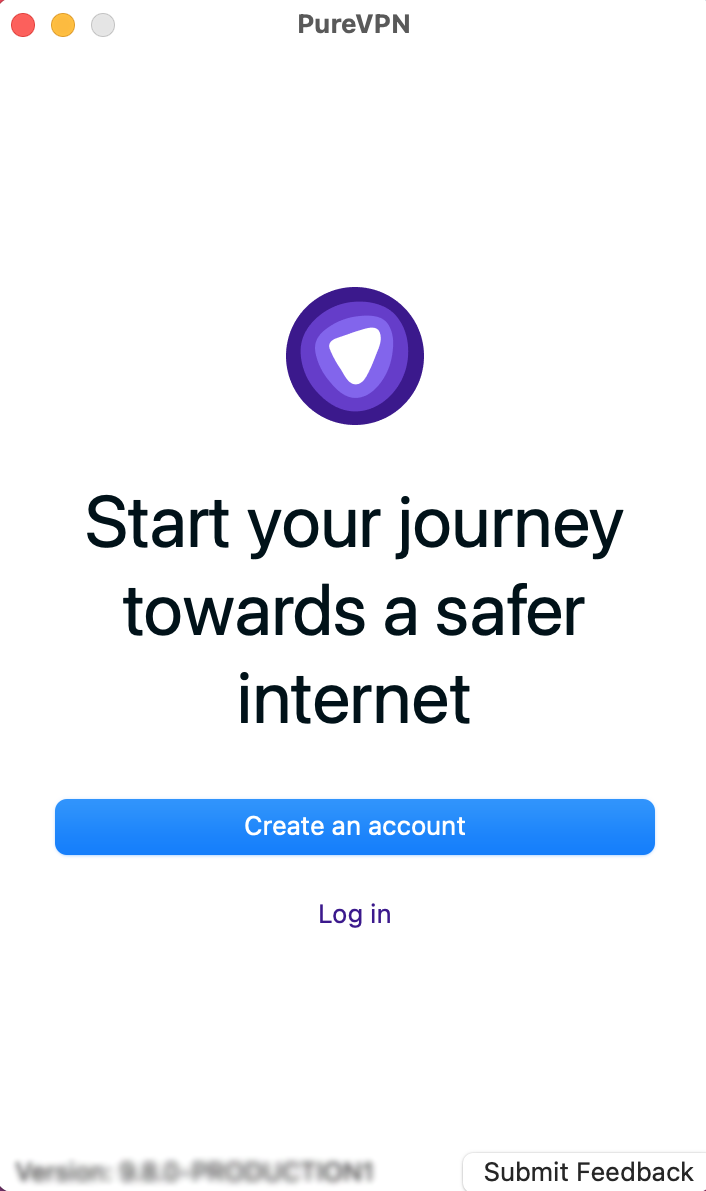
\includegraphics[width=10cm]{24.png}
\centering
\caption{Вход в систему}
\label{fig:29}
\end{figure}

Вы будете перенаправлены в ваш браузер по умолчанию для входа в систему.

Введите свой адрес электронной почты PureVPN и пароль (используйте адрес электронной почты и пароль, которые вы указали при покупке).
\item После ввода данных учетной записи нажмите Отправить:  Рисунок(\ref{fig:30})
\begin{figure}[H]
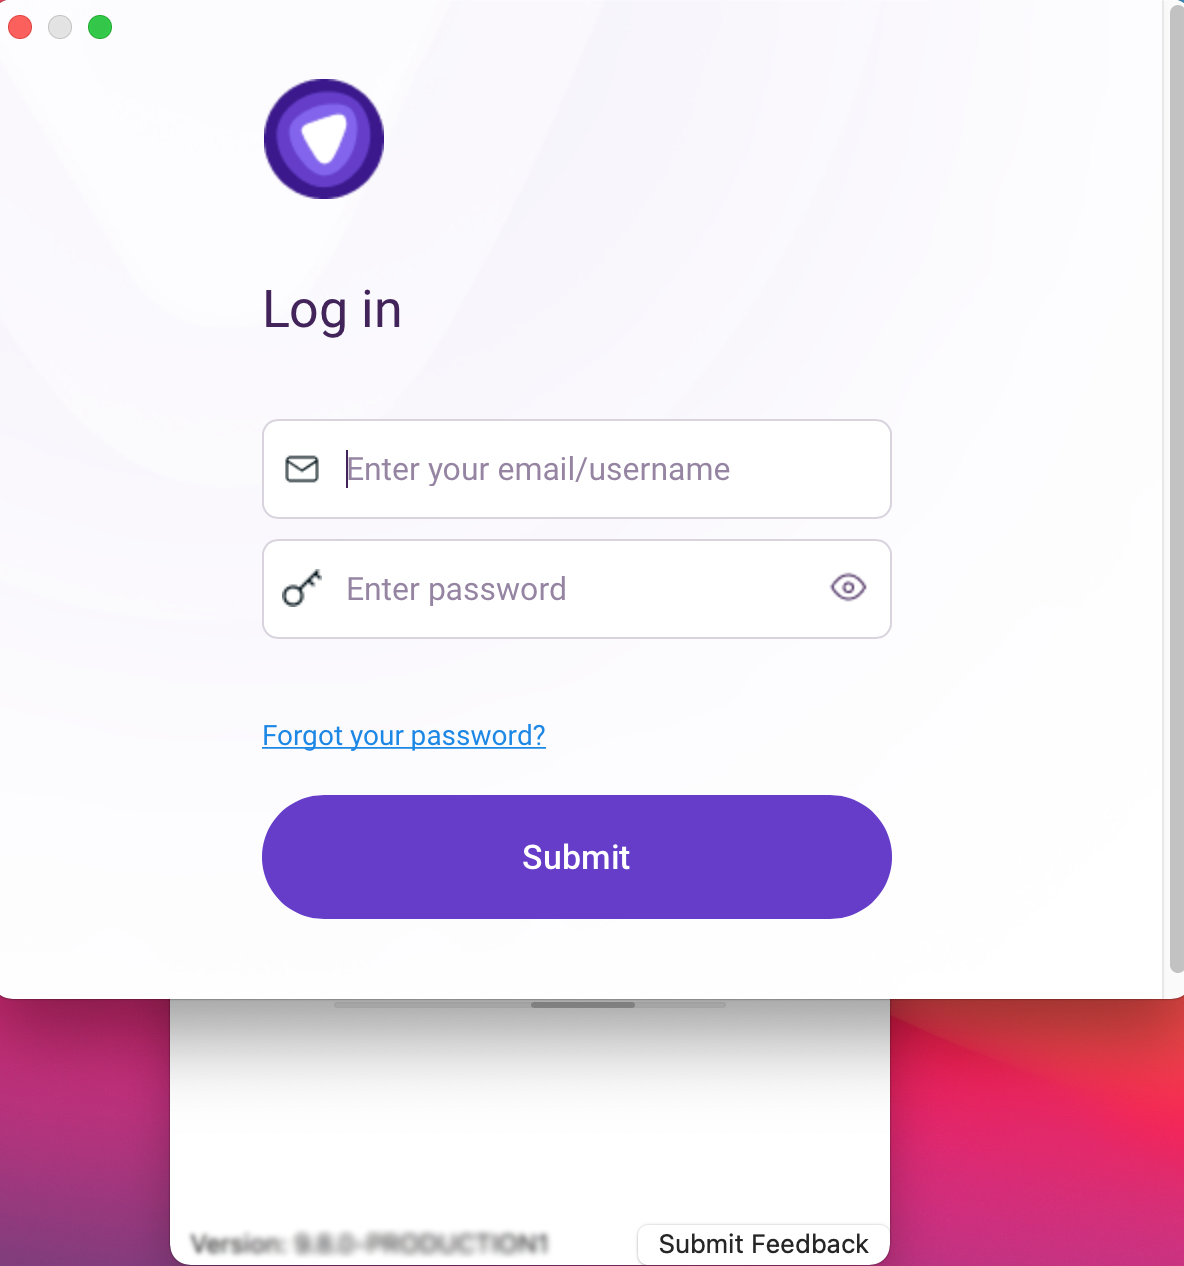
\includegraphics[width=10cm]{25.png}
\centering
\caption{Вход в учетную запись}
\label{fig:30}
\end{figure}
\item Как только вы нажмете Отправить, автоматически откроется приложение PureVPN, и вы войдете в приложение.

Примечание:

Если у вас несколько подписок на одно электронное письмо, вам будет предоставлена возможность выбрать учетную запись, в которую вы хотите войти.
\item Нажмите на желаемое имя пользователя PureVPN, затем нажмите Выбрать учетную запись:  Рисунок(\ref{fig:31})
\begin{figure}[H]
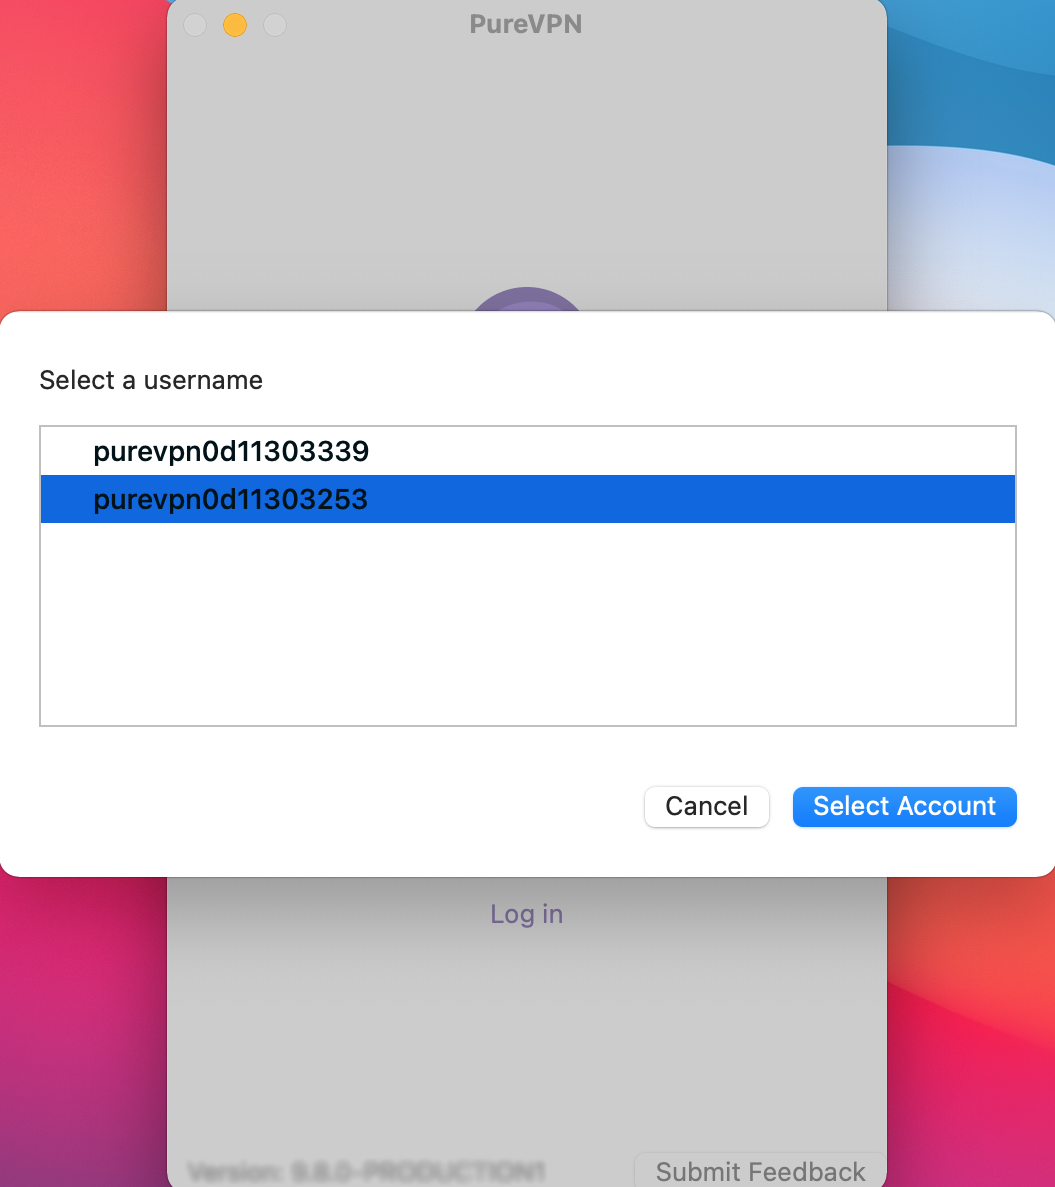
\includegraphics[width=10cm]{26.png}
\centering
\caption{Выбор учетной записи}
\label{fig:31}
\end{figure}
\item Выберите назначение, которое наилучшим образом соответствует вашим потребностям в VPN:  Рисунок(\ref{fig:32})
\begin{figure}[H]
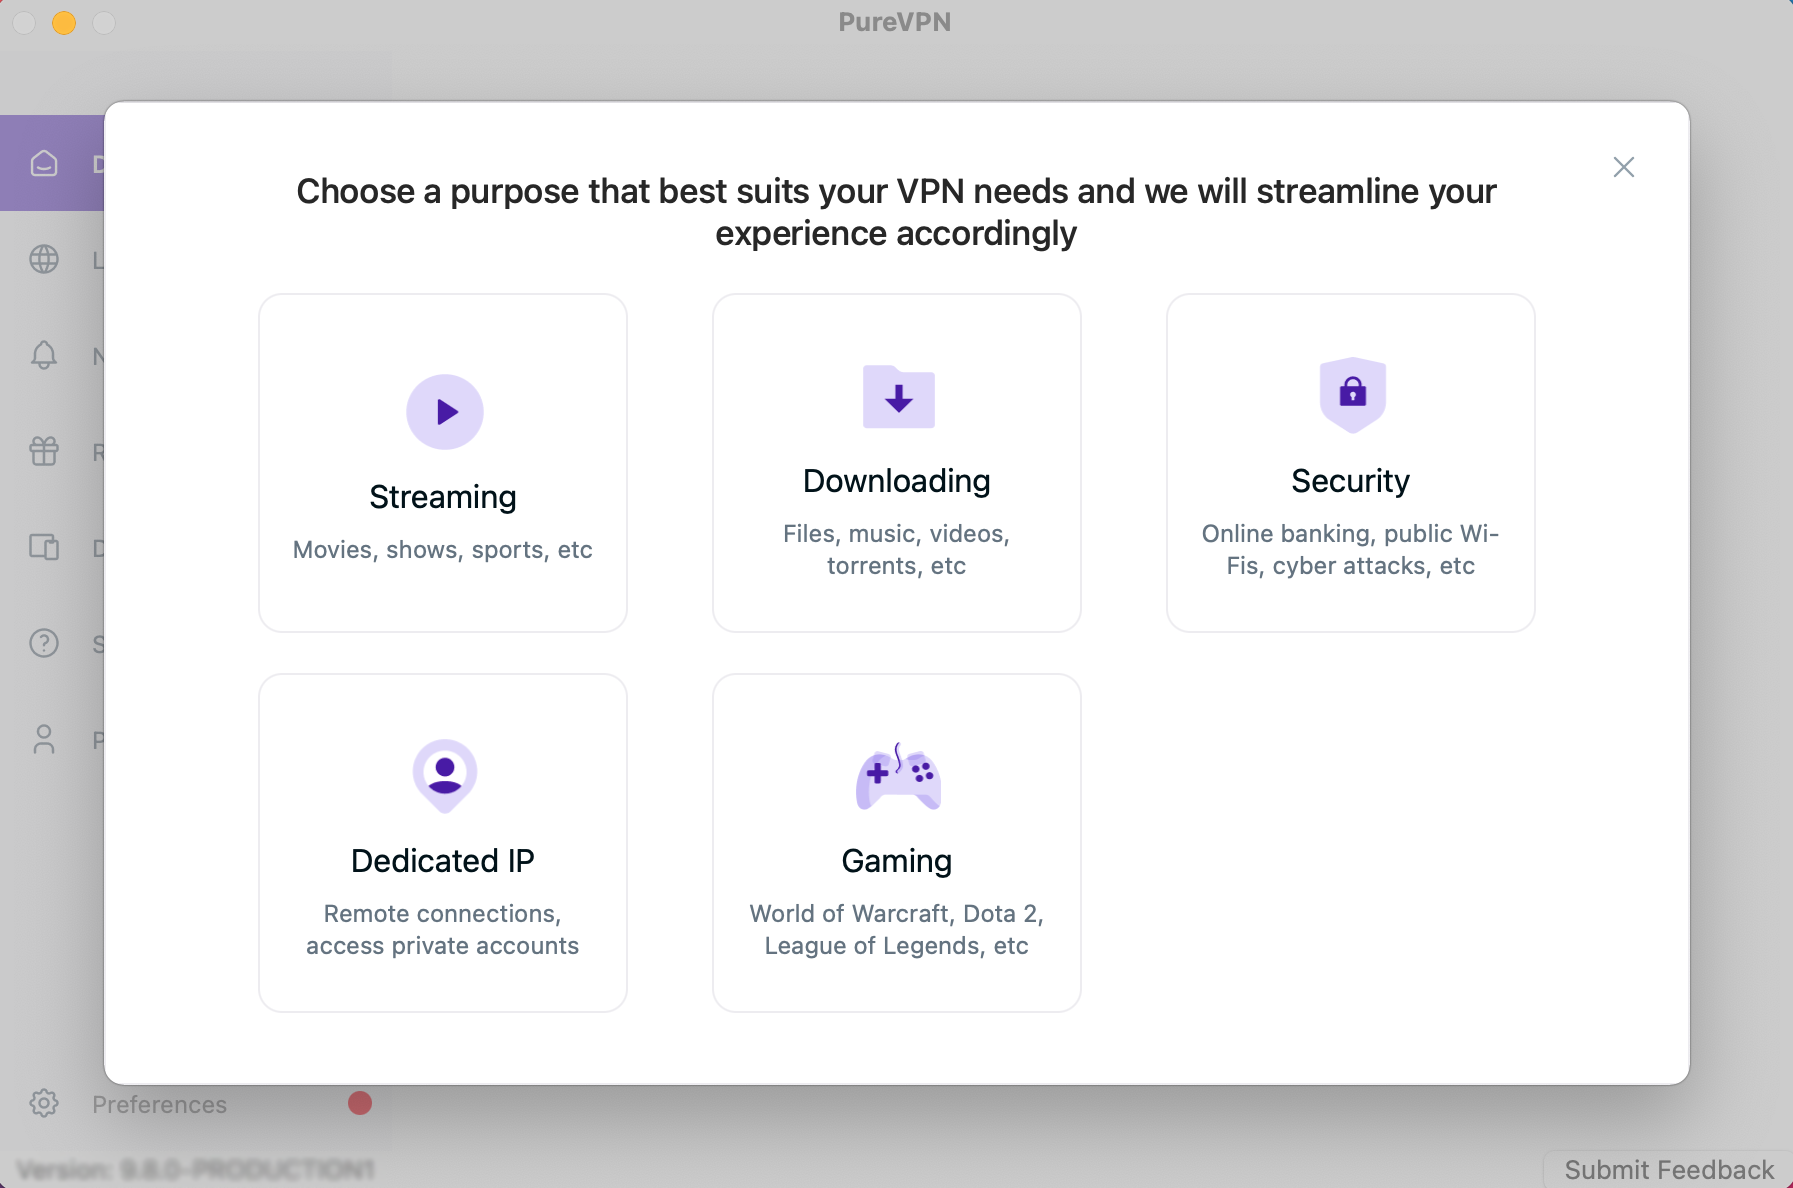
\includegraphics[width=14cm]{27.png}
\centering
\caption{Потребности}
\label{fig:32}
\end{figure}
\item Теперь вы вошли в приложение PureVPN:  Рисунок(\ref{fig:33})
\begin{figure}[H]
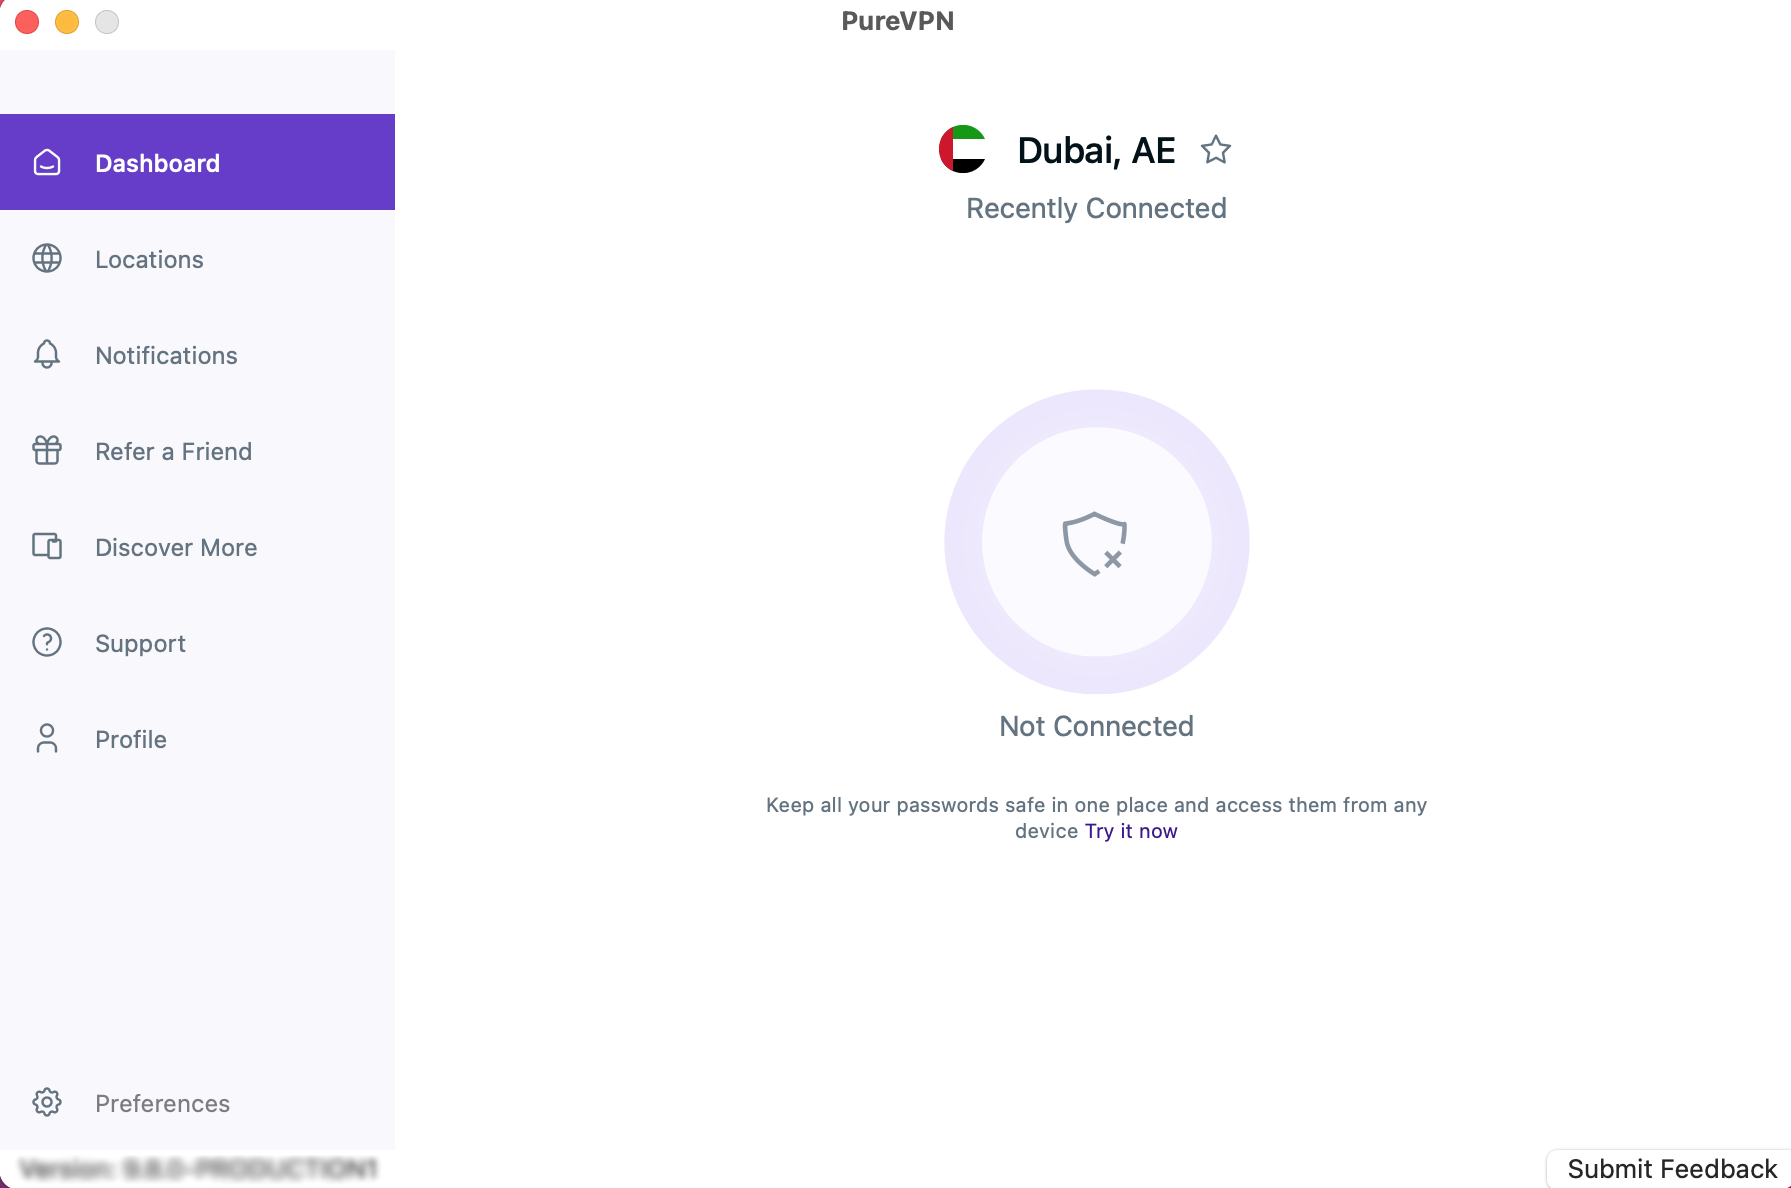
\includegraphics[width=14cm]{28.png}
\centering
\caption{Главная страница приложения}
\label{fig:33}
\end{figure}
\end{itemize}

\subsection{Выход из приложения PureVPN} 
Хотите выйти из приложения PureVPN? Вот упрощенный способ, которому вы должны следовать, чтобы выйти из приложения PureVPN.
\begin{itemize}
\item Щелкните профиль на левой панели приложения PureVPN:  Рисунок(\ref{fig:34})
\begin{figure}[H]
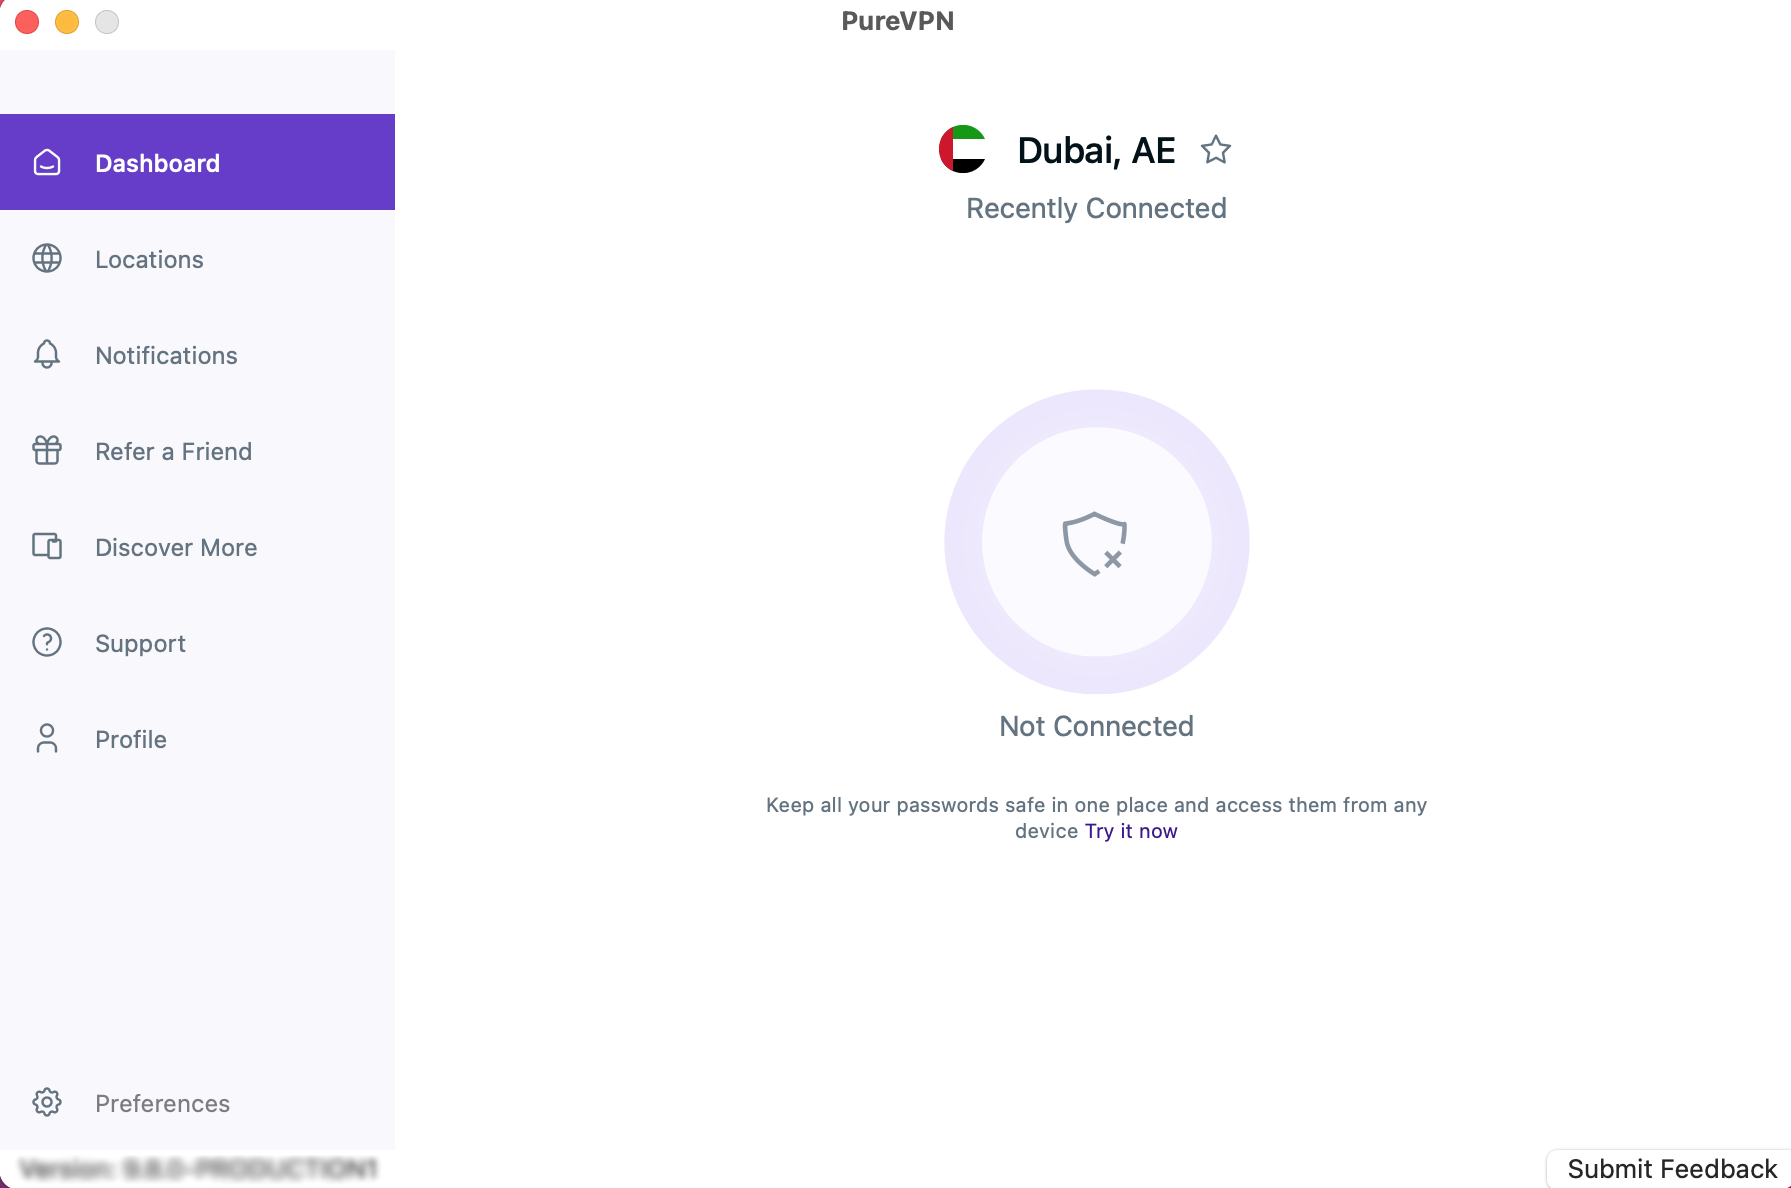
\includegraphics[width=12cm]{28.png}
\centering
\caption{Главная страница приложения}
\label{fig:34}
\end{figure}
\item В разделе профиля вы сможете увидеть опцию выхода из системы. Нажмите Выход из системы, чтобы продолжить:  Рисунок(\ref{fig:35})
\begin{figure}[H]
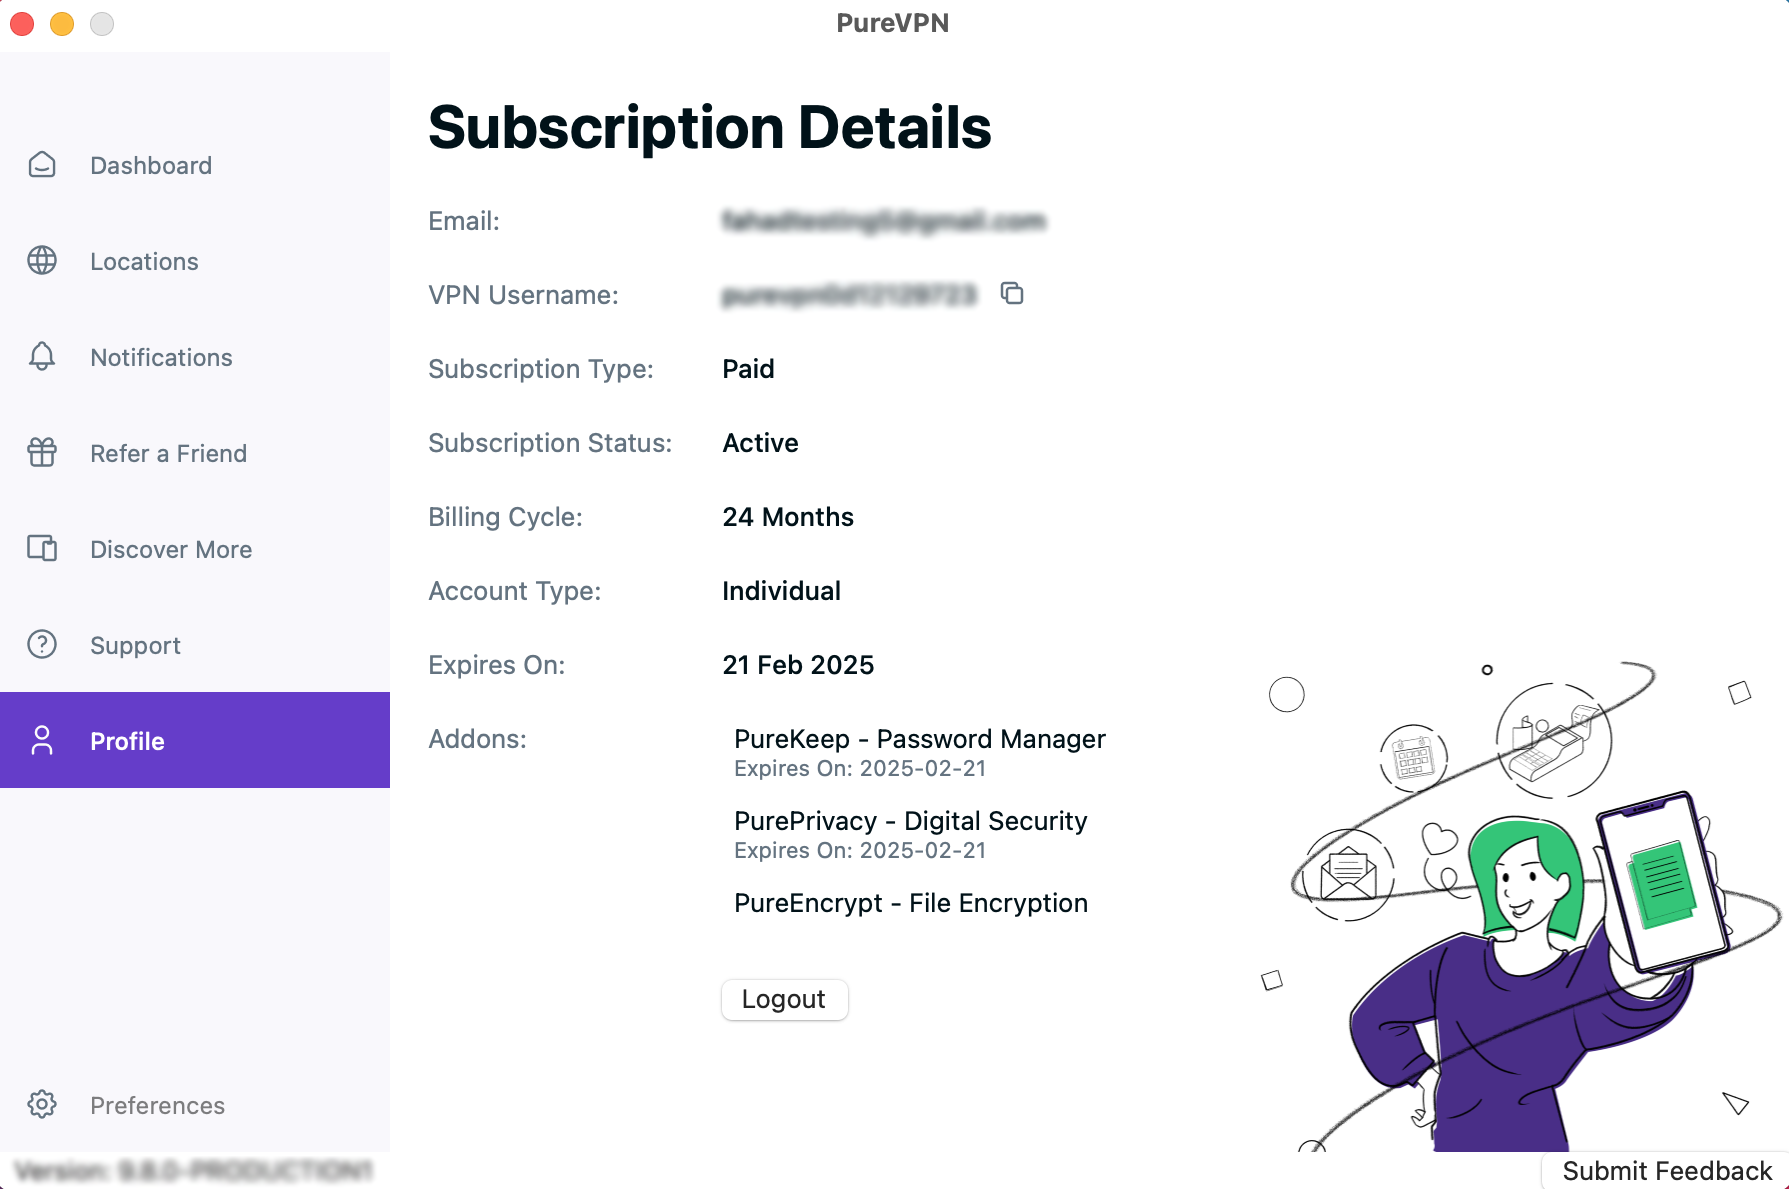
\includegraphics[width=12cm]{29.png}
\centering
\caption{Выход из системы}
\label{fig:35}
\end{figure}
\item Вы успешно вышли из приложения PureVPN:  Рисунок(\ref{fig:36})
\begin{figure}[H]
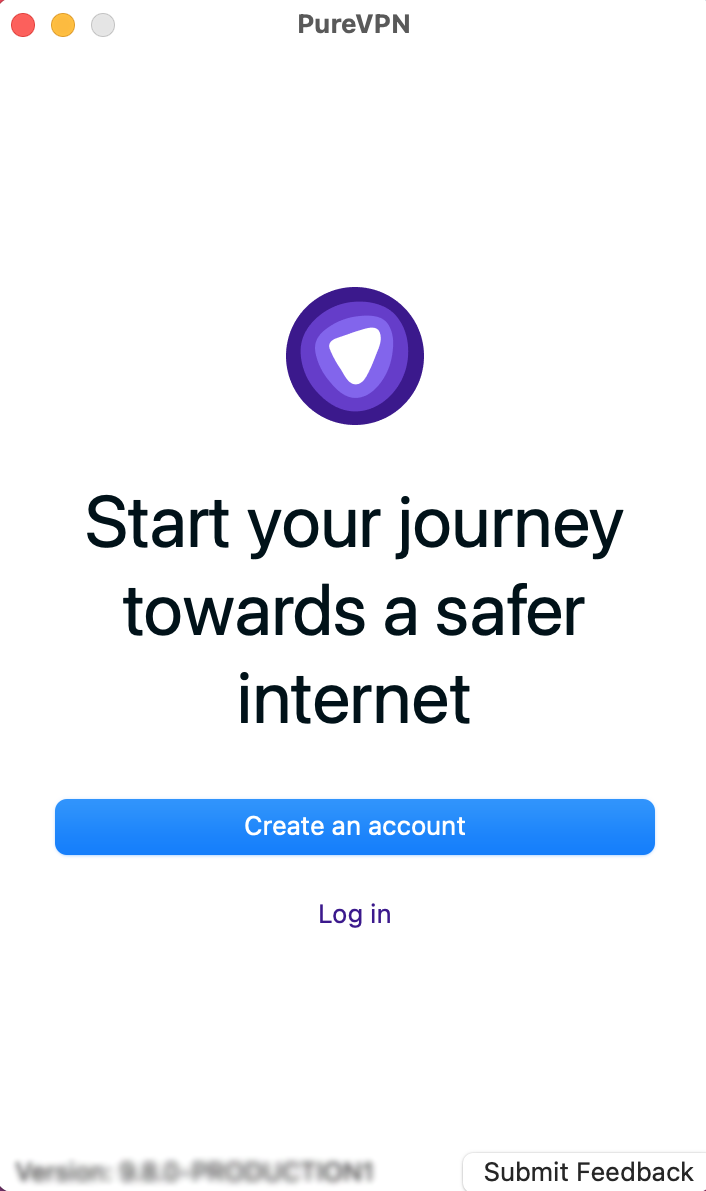
\includegraphics[width=8cm]{24.png}
\centering
\caption{Успешный выход из приложения}
\label{fig:36}
\end{figure}
\end{itemize}

\subsection{Проверьте сведения о подписке в приложении PureVPN} 
Ищете способ просмотреть сведения о вашей подписке в приложении PureVPN? Следуйте приведенным ниже инструкциям, чтобы иметь возможность просматривать сведения о вашей подписке в приложении PureVPN.
\begin{itemize}
\item Щелкните по значку пользователя на левой панели приложения PureVPN:  Рисунок(\ref{fig:37})
\begin{figure}[H]
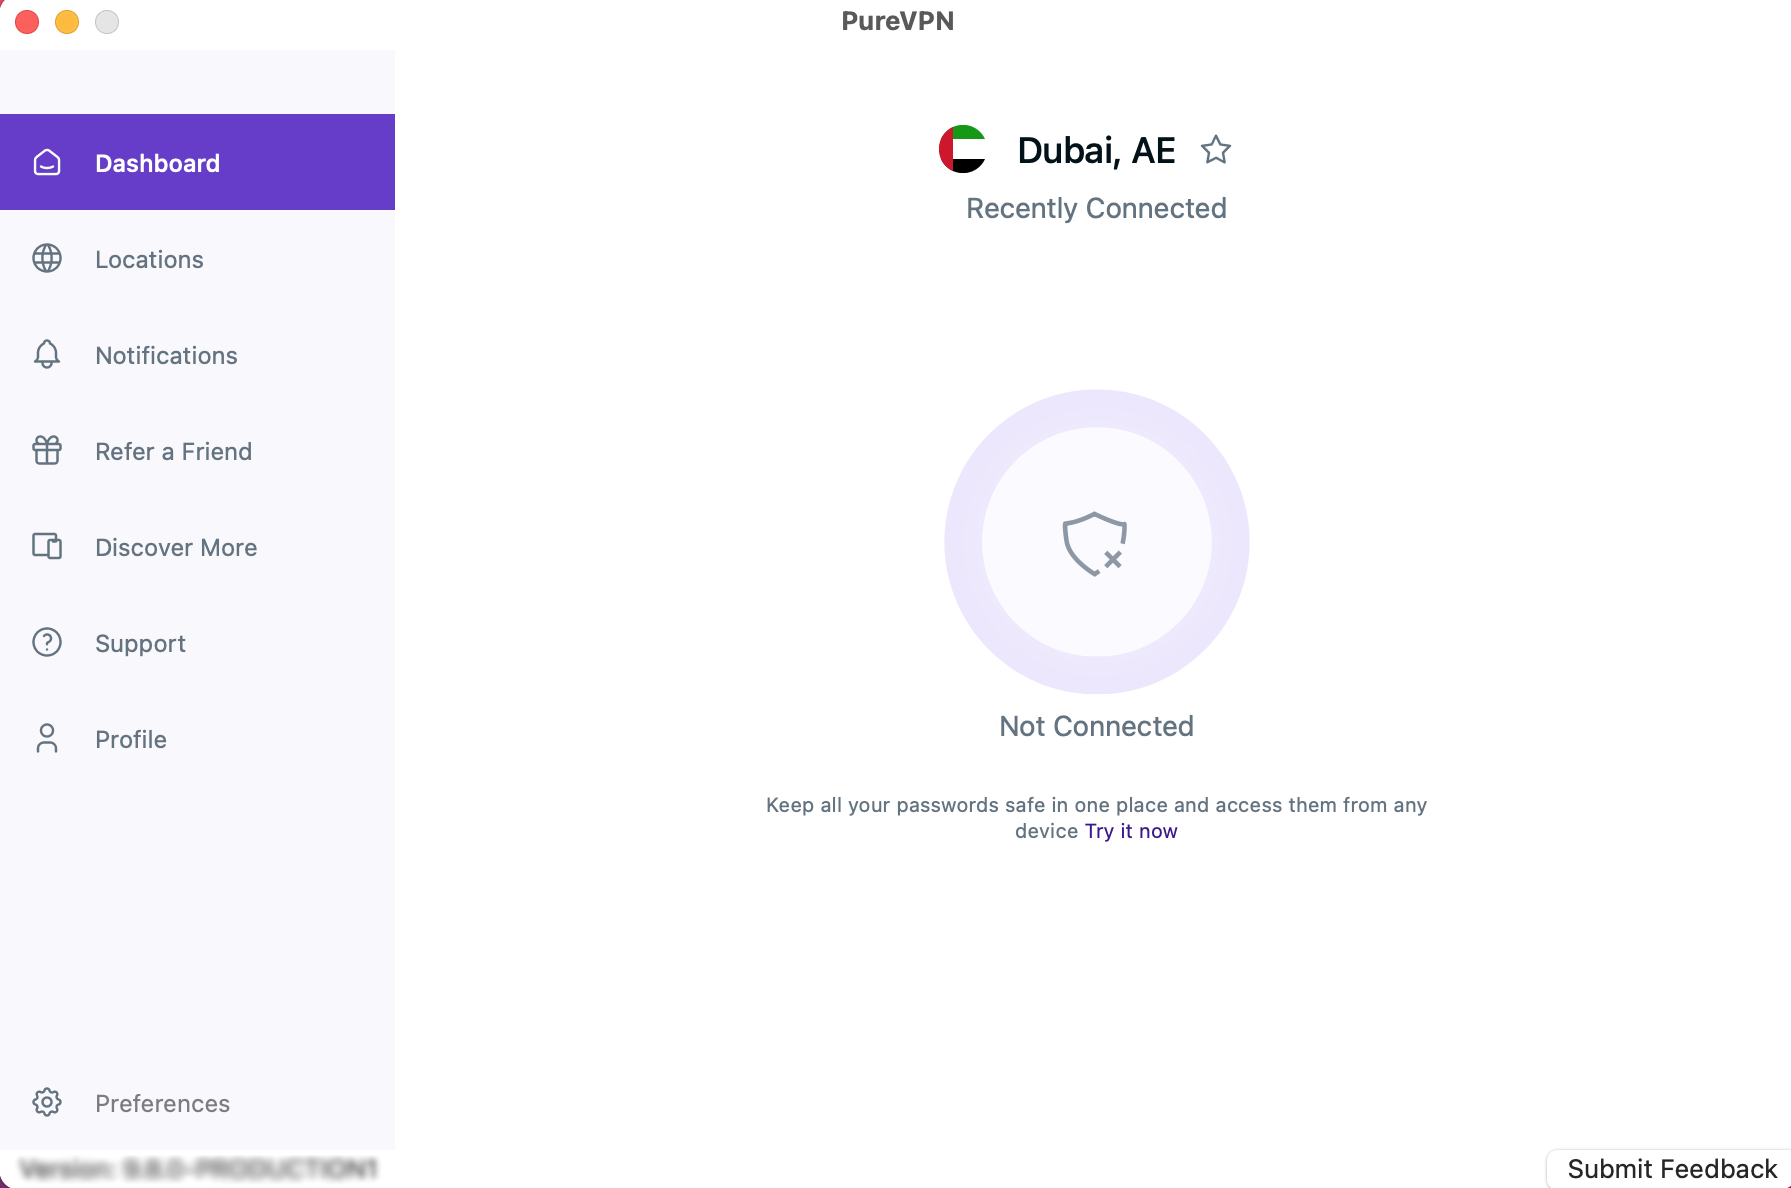
\includegraphics[width=12cm]{28.png}
\centering
\caption{Главная страница приложения}
\label{fig:37}
\end{figure}
\item В разделе профиля вы сможете просмотреть сведения о подписке.
\item Ниже приведены сведения, которые будут видны в разделе Профиля:  Рисунок(\ref{fig:38})
\begin{enumerate}
\item Электронная почта
\item Имя пользователя VPN
\item Тип подписки
\item Статус подписки
\item Цикл выставления счетов
\item Срок действия подписки истек
\item Аддоны
\end{enumerate}
\begin{figure}[H]
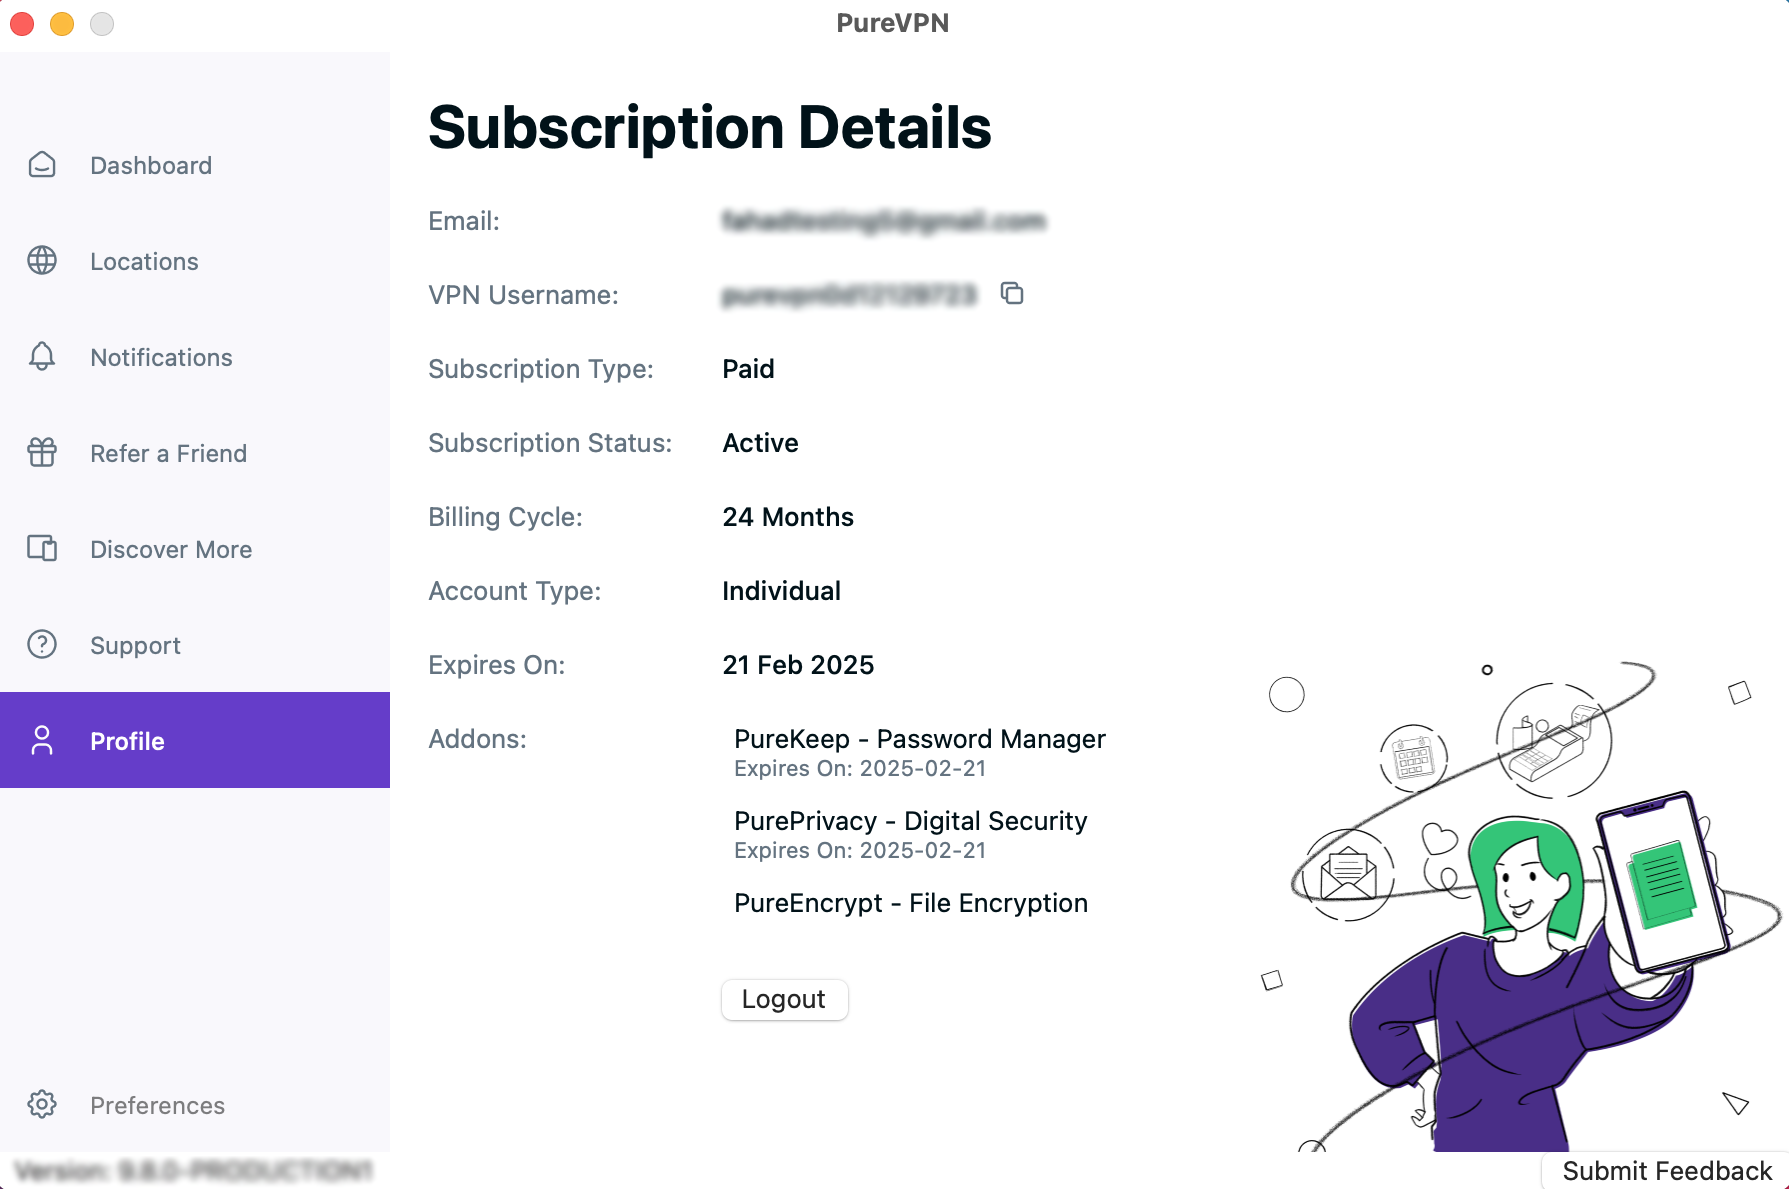
\includegraphics[width=12cm]{29.png}
\centering
\caption{Сведения о подписке}
\label{fig:38}
\end{figure}
\end{itemize}

\section{Android}

\subsection{Загрузите и установите приложение PureVPN} 
Чтобы загрузить и установить приложение PureVPN, выполните следующие действия:
\begin{itemize}
\item Для начала найдите на своем устройстве приложение Play Store и откройте его:  Рисунок(\ref{fig:39})
\begin{figure}[H]
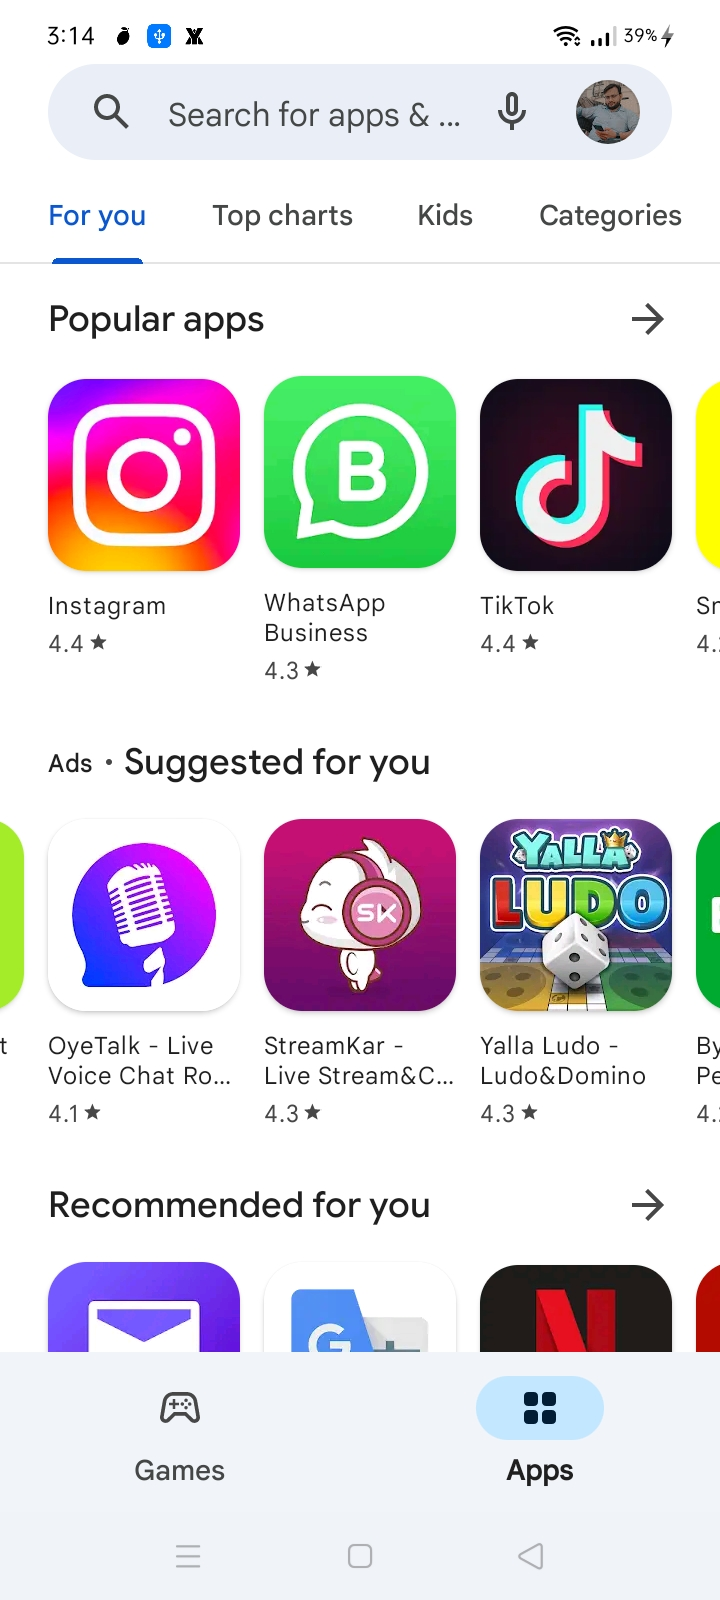
\includegraphics[width=8cm]{30.png}
\centering
\caption{Play Store}
\label{fig:39}
\end{figure}

Введите PureVPN в строку поиска и выберите первый результат, который появится в списке.
\item Нажмите установить, как только найдете нужное:  Рисунок(\ref{fig:40})
\begin{figure}[H]
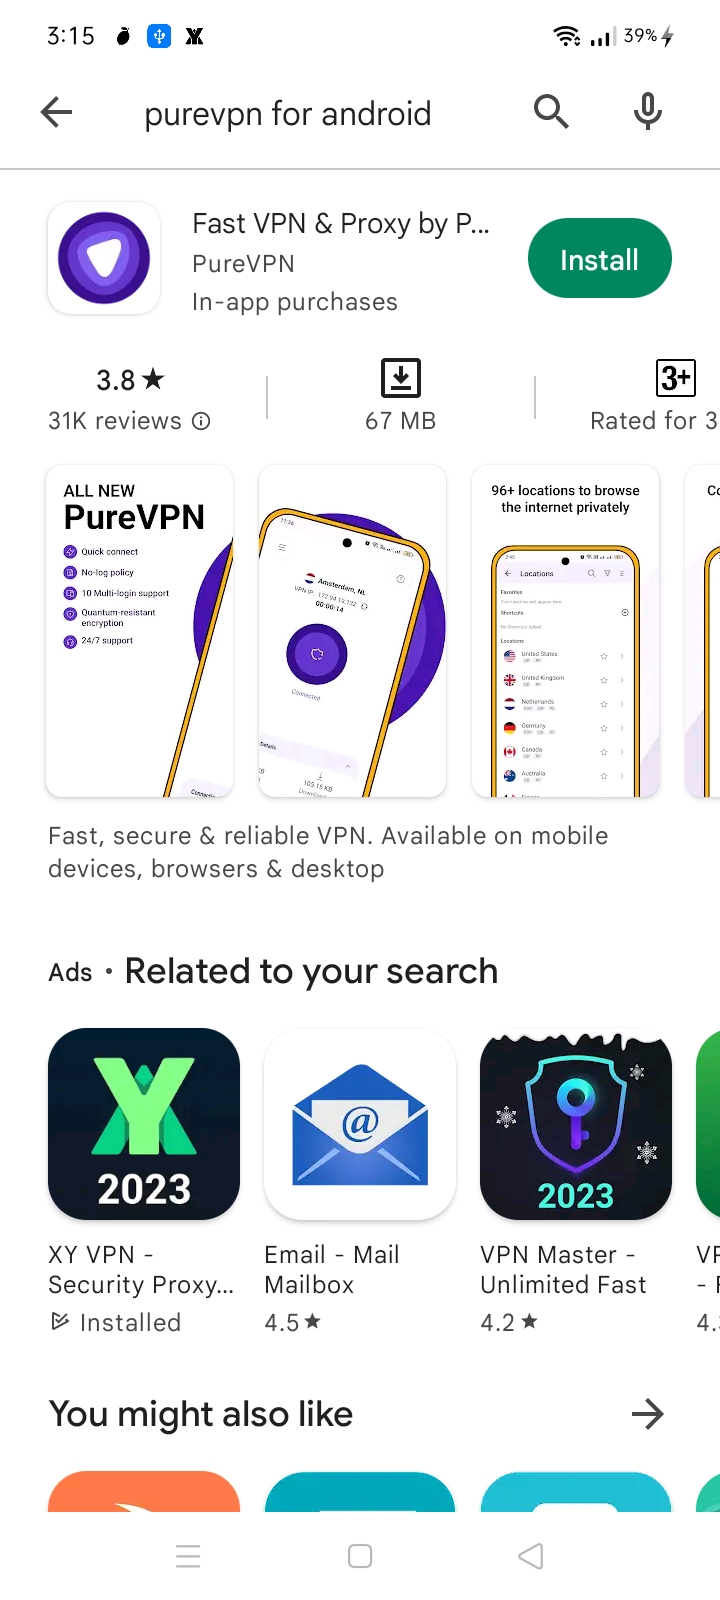
\includegraphics[width=8cm]{31.png}
\centering
\caption{Кнопка установить}
\label{fig:40}
\end{figure}
\item Приложение PureVPN успешно установлено:  Рисунок(\ref{fig:41})
\begin{figure}[H]
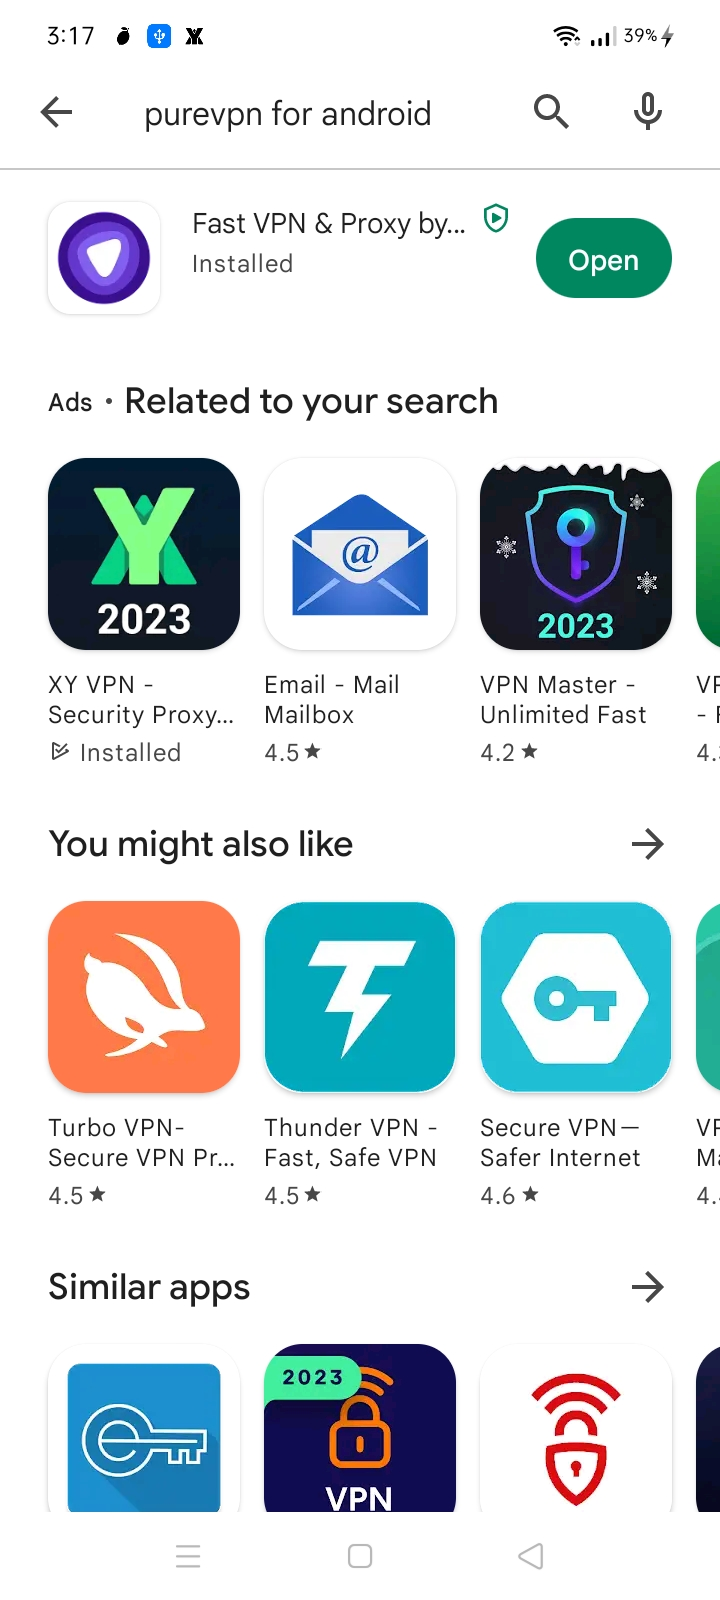
\includegraphics[width=8cm]{32.png}
\centering
\caption{Приложение установлено}
\label{fig:41}
\end{figure}
\end{itemize}

\subsection{Войдите в приложение PureVPN} 
Как только приложение установлено, вы можете приступить к запуску приложения и войти в него.
\begin{itemize}
\item Запустите приложение PureVPN .
\item Нажмите Есть учетная запись? Вход:  Рисунок(\ref{fig:42})
\begin{figure}[H]
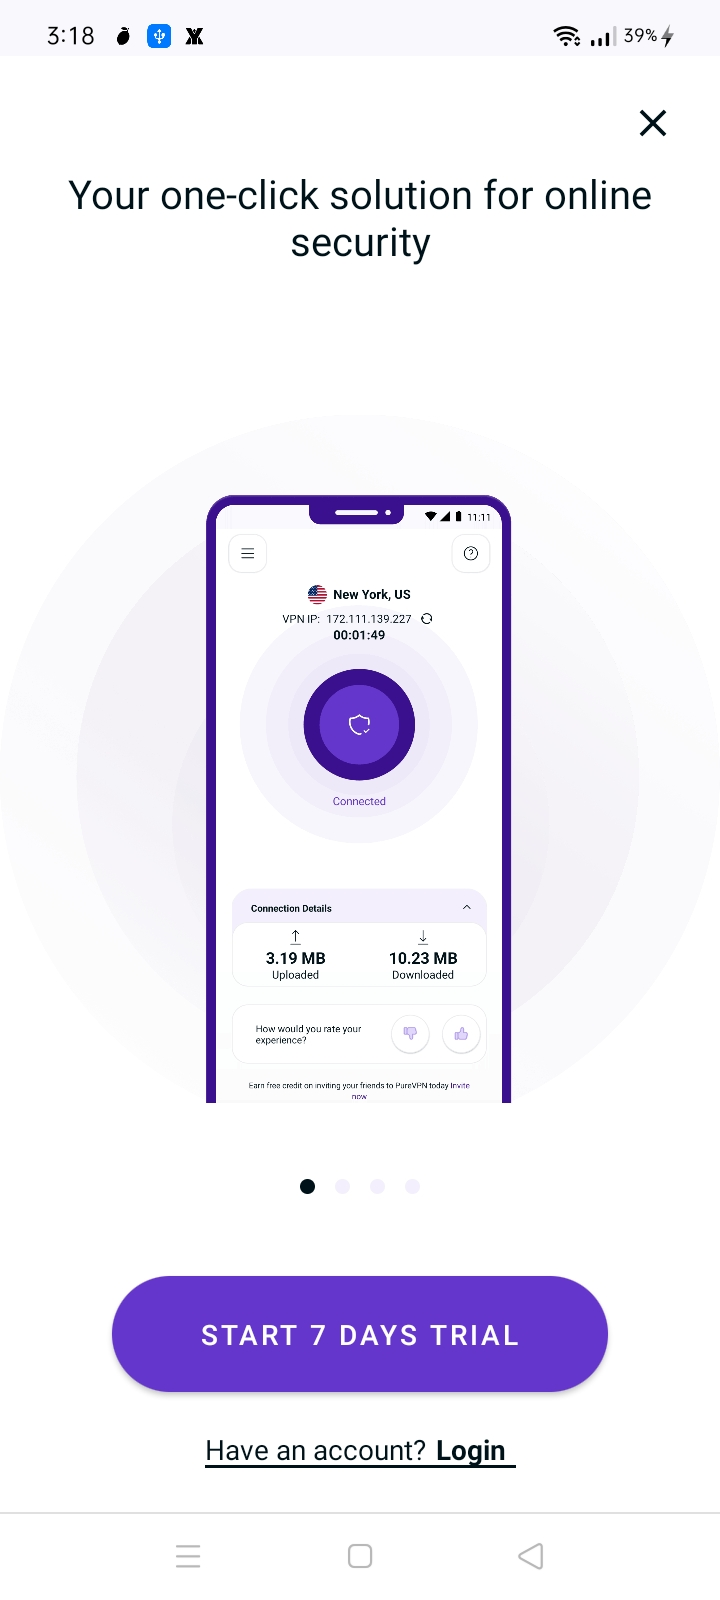
\includegraphics[width=8cm]{33.png}
\centering
\caption{Вход}
\label{fig:42}
\end{figure}
\item Вы будете перенаправлены в ваш браузер по умолчанию для входа в систему.
\item Введите свой адрес электронной почты PureVPN и пароль (используйте адрес электронной почты и пароль, которые вы указали при покупке).
\item После ввода данных учетной записи нажмите Отправить:  Рисунок(\ref{fig:43})
\begin{figure}[H]
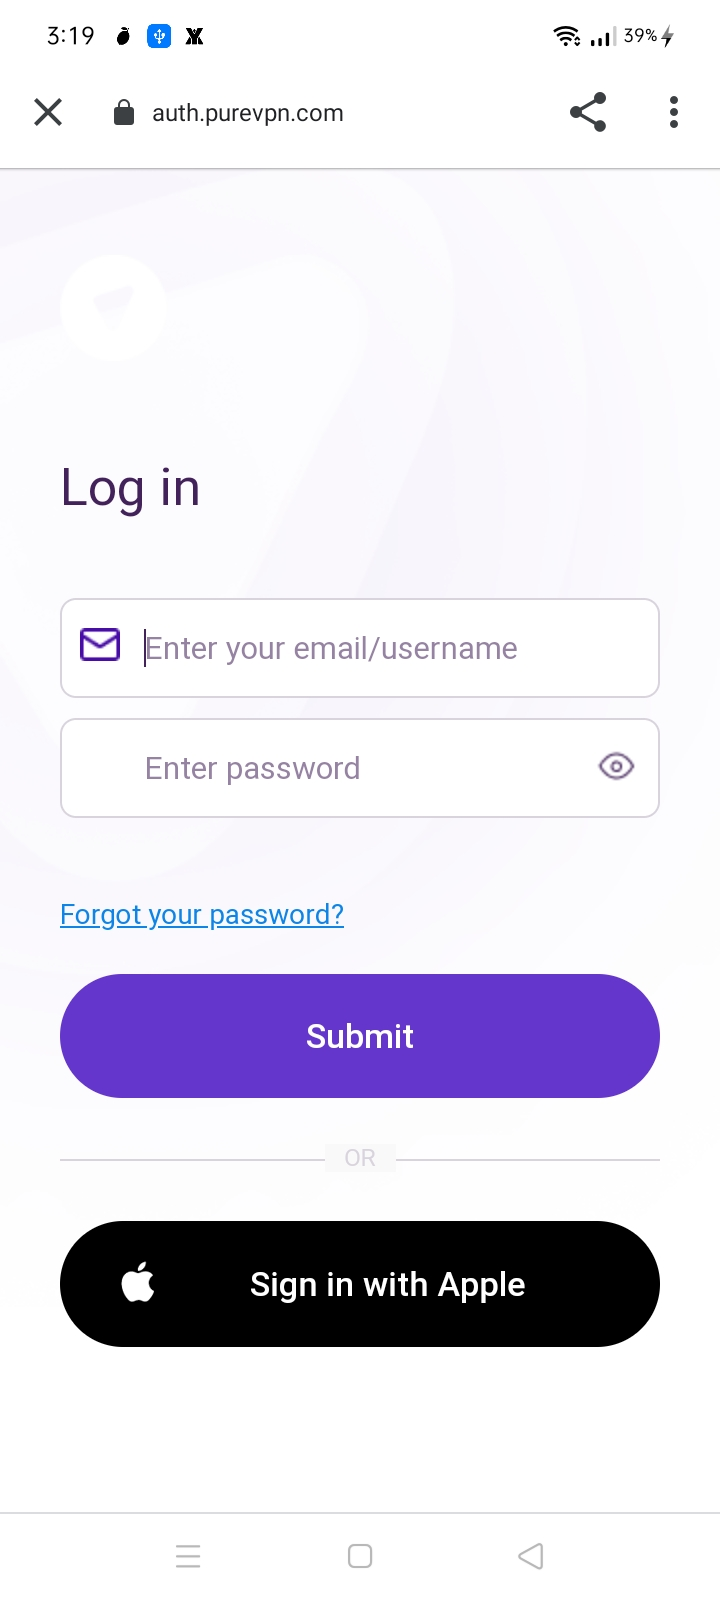
\includegraphics[width=8cm]{34.png}
\centering
\caption{Отправить}
\label{fig:43}
\end{figure}
\item Как только вы нажмете Отправить, автоматически откроется приложение PureVPN, и вы войдете в приложение:  Рисунок(\ref{fig:44})
\begin{figure}[H]
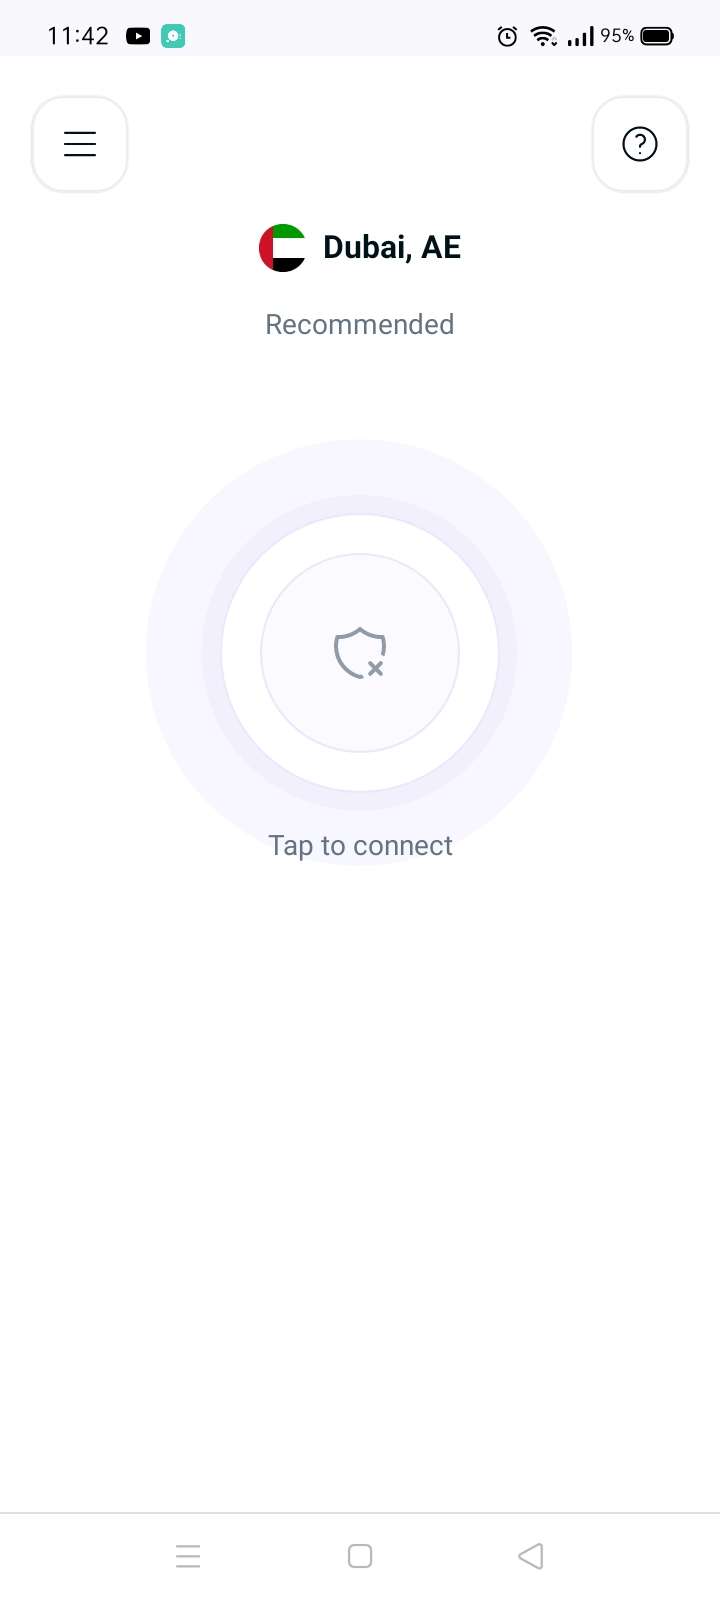
\includegraphics[width=8cm]{35.png}
\centering
\caption{Главная страница приложения}
\label{fig:44}
\end{figure}

Примечание:

Если у вас несколько учетных записей, вам будет предложено выбрать свое имя пользователя PureVPN:  Рисунок(\ref{fig:45})
\begin{figure}[H]
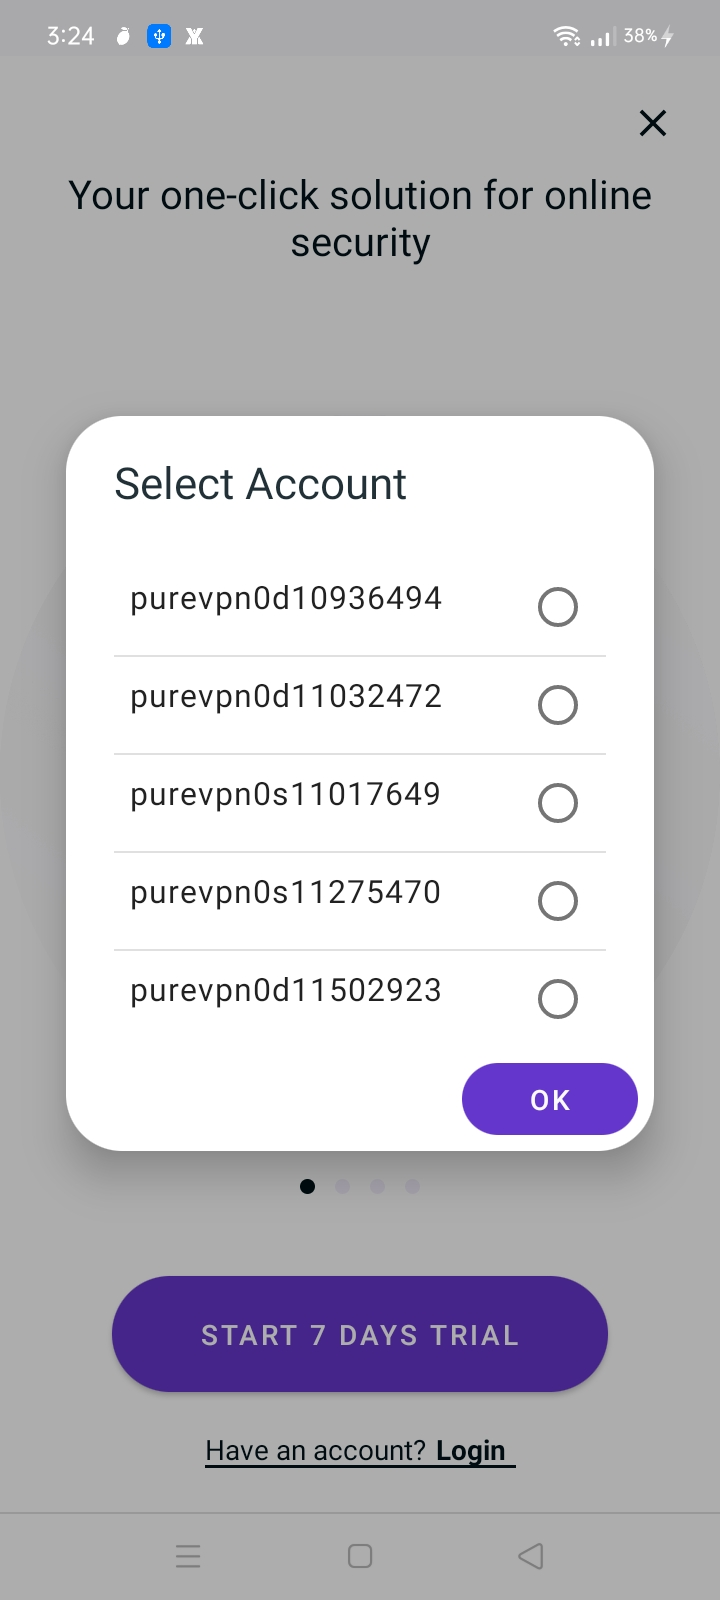
\includegraphics[width=8cm]{36.png}
\centering
\caption{Выбор учетной записи}
\label{fig:45}
\end{figure}
\item Выберите цель, которая наилучшим образом соответствует вашим потребностям в VPN:  Рисунок(\ref{fig:46})
\begin{figure}[H]
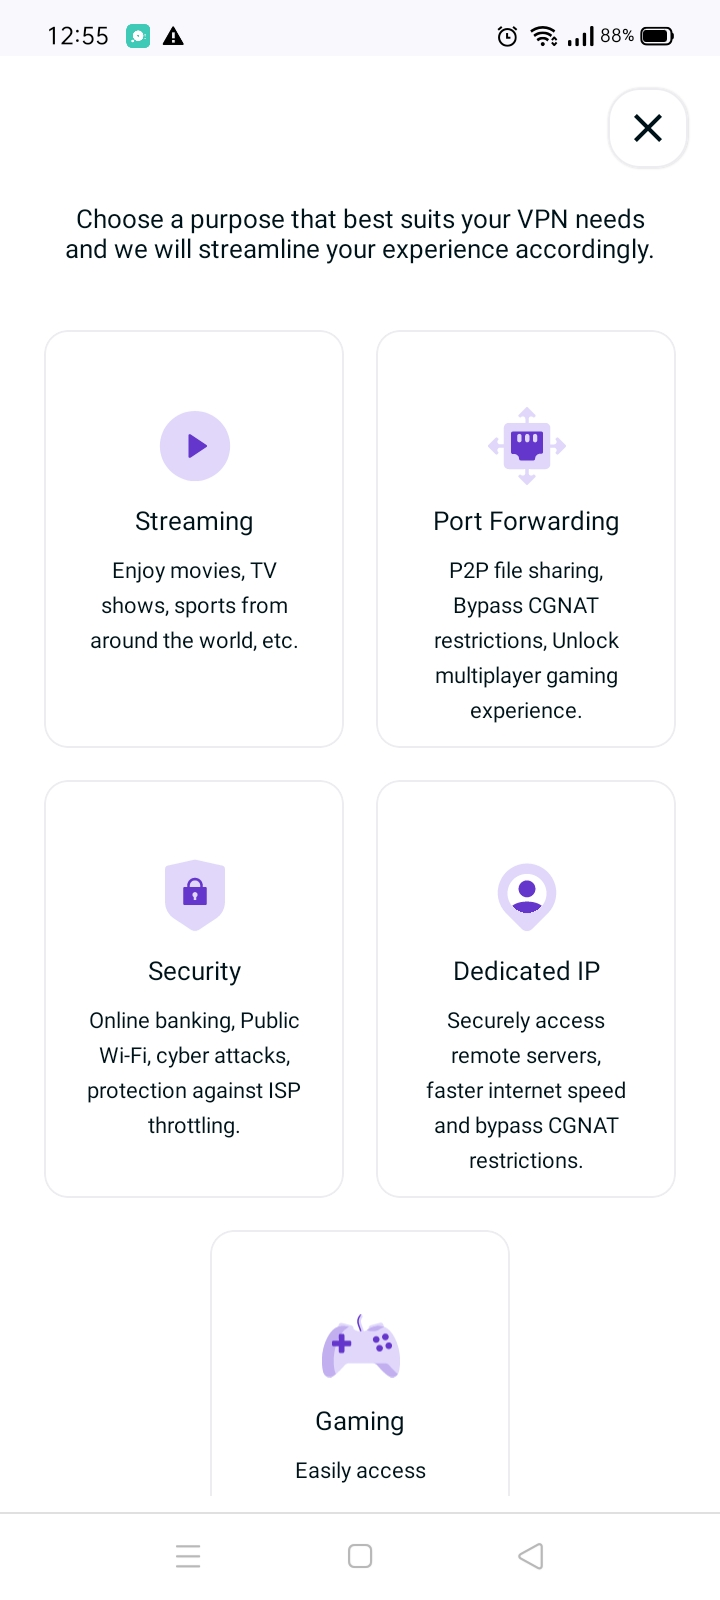
\includegraphics[width=8cm]{37.png}
\centering
\caption{Потребности}
\label{fig:46}
\end{figure}
\item После завершения вы войдете в приложение PureVPN:  Рисунок(\ref{fig:47})
\begin{figure}[H]
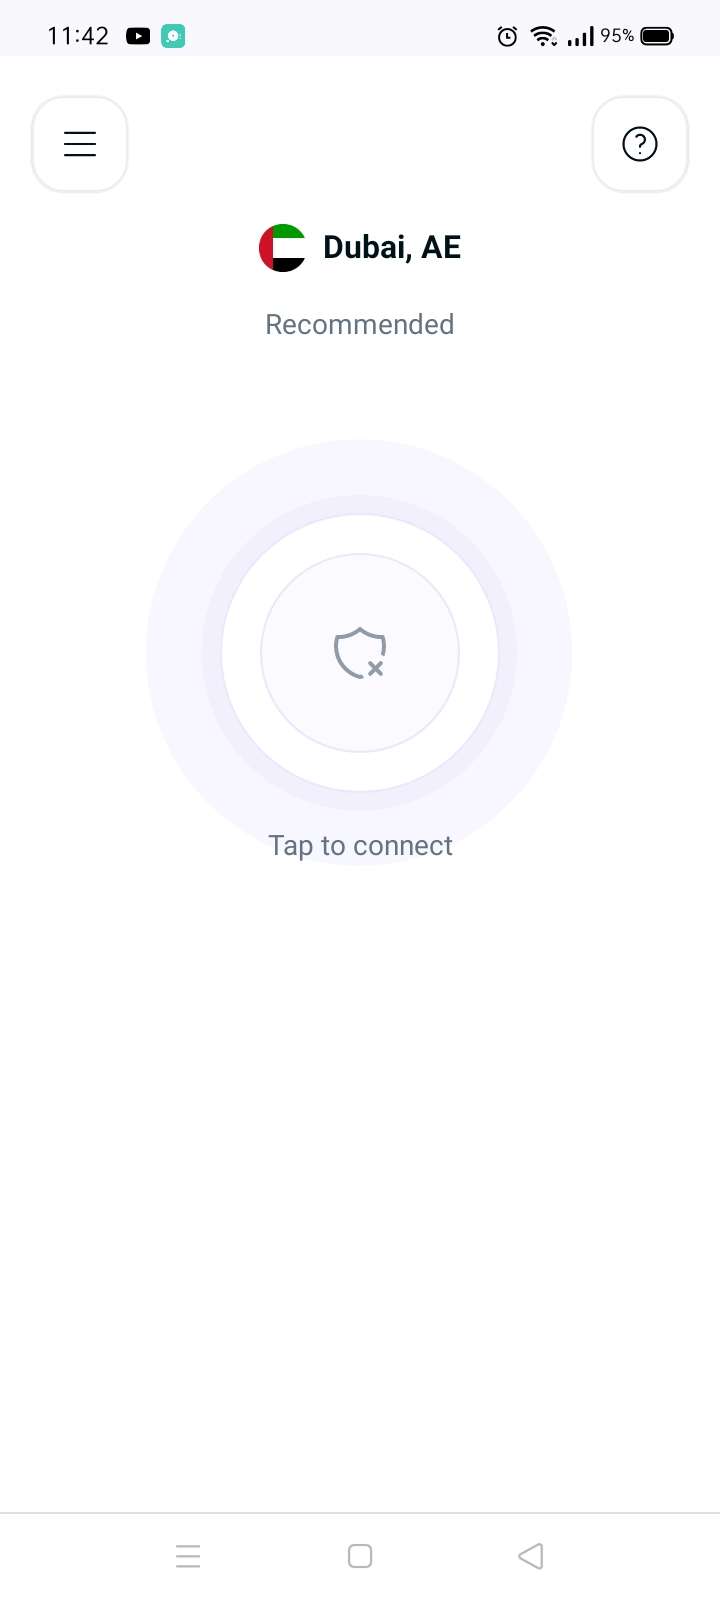
\includegraphics[width=8cm]{35.png}
\centering
\caption{Главная страница приложения}
\label{fig:47}
\end{figure}
\end{itemize}

\subsection{Выход из приложения PureVPN} 
Вот как легко и без лишних хлопот выйти из приложения PureVPN.
\begin{itemize}
\item Коснитесь значка гамбургера в левом верхнем углу:  Рисунок(\ref{fig:48})
\begin{figure}[H]
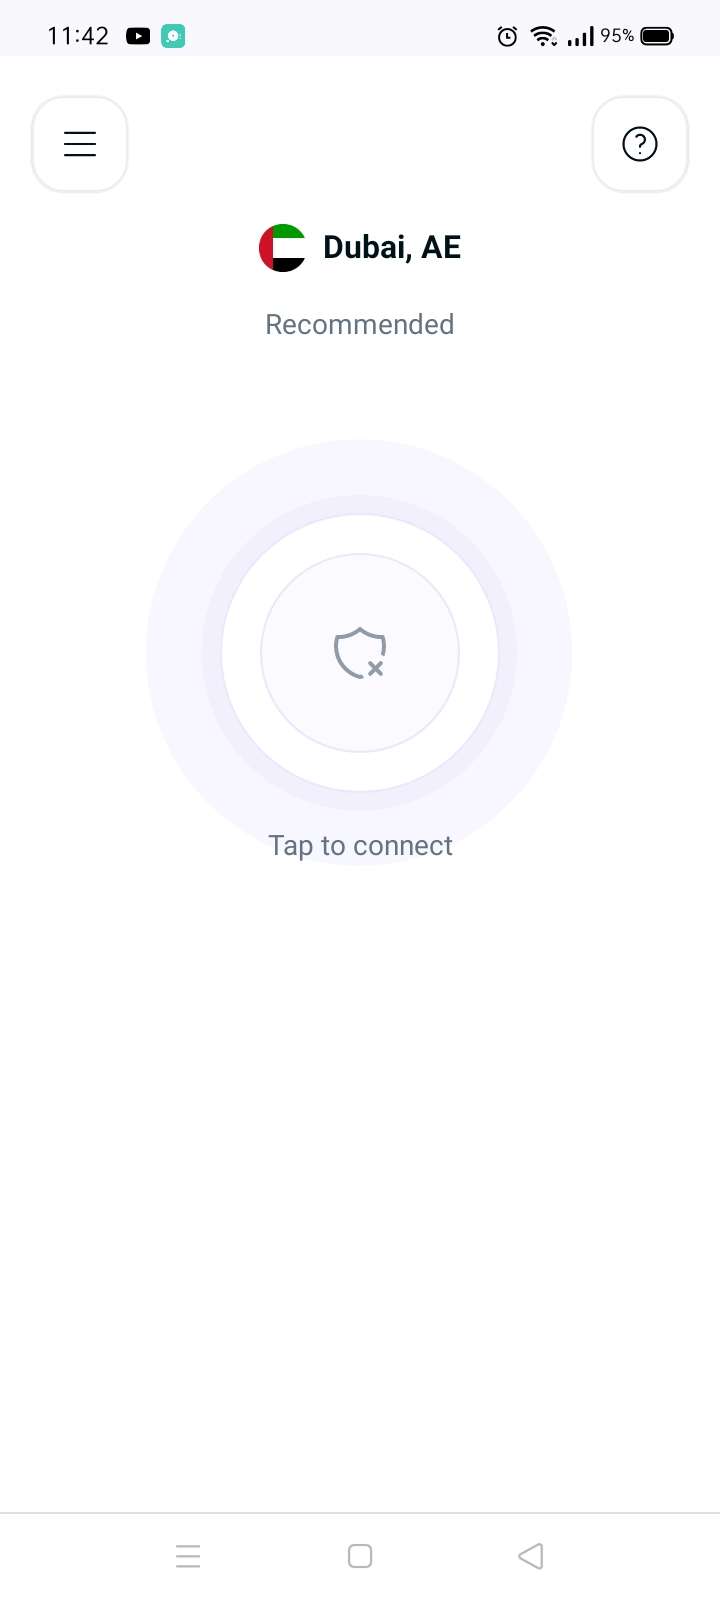
\includegraphics[width=8cm]{35.png}
\centering
\caption{Значок гамбургера}
\label{fig:48}
\end{figure}
\item Коснитесь данных учетной записи:  Рисунок(\ref{fig:49})
\begin{figure}[H]
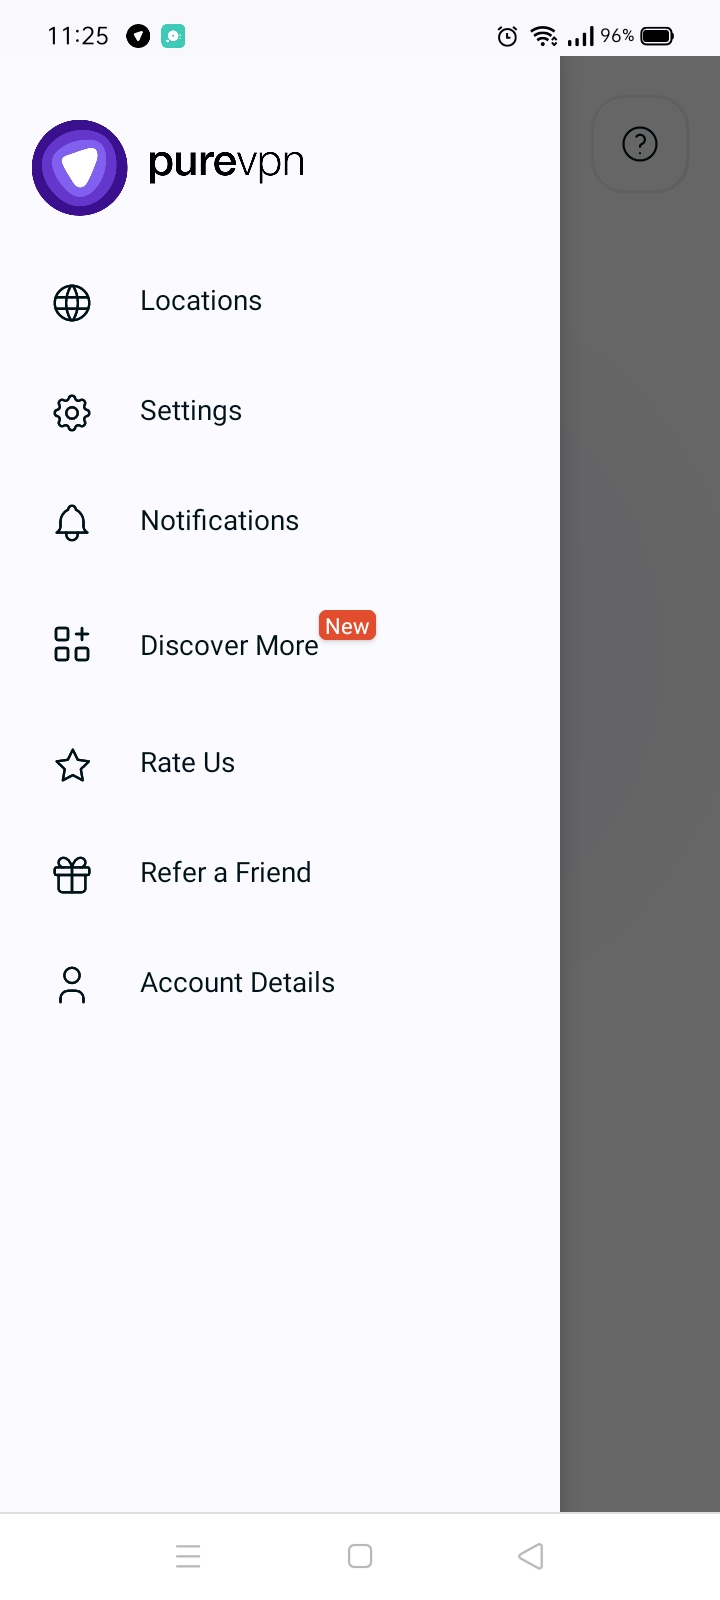
\includegraphics[width=8cm]{38.png}
\centering
\caption{Данные учетной записи}
\label{fig:49}
\end{figure}
\item Нажмите Выйти из системы:  Рисунок(\ref{fig:50})
\begin{figure}[H]
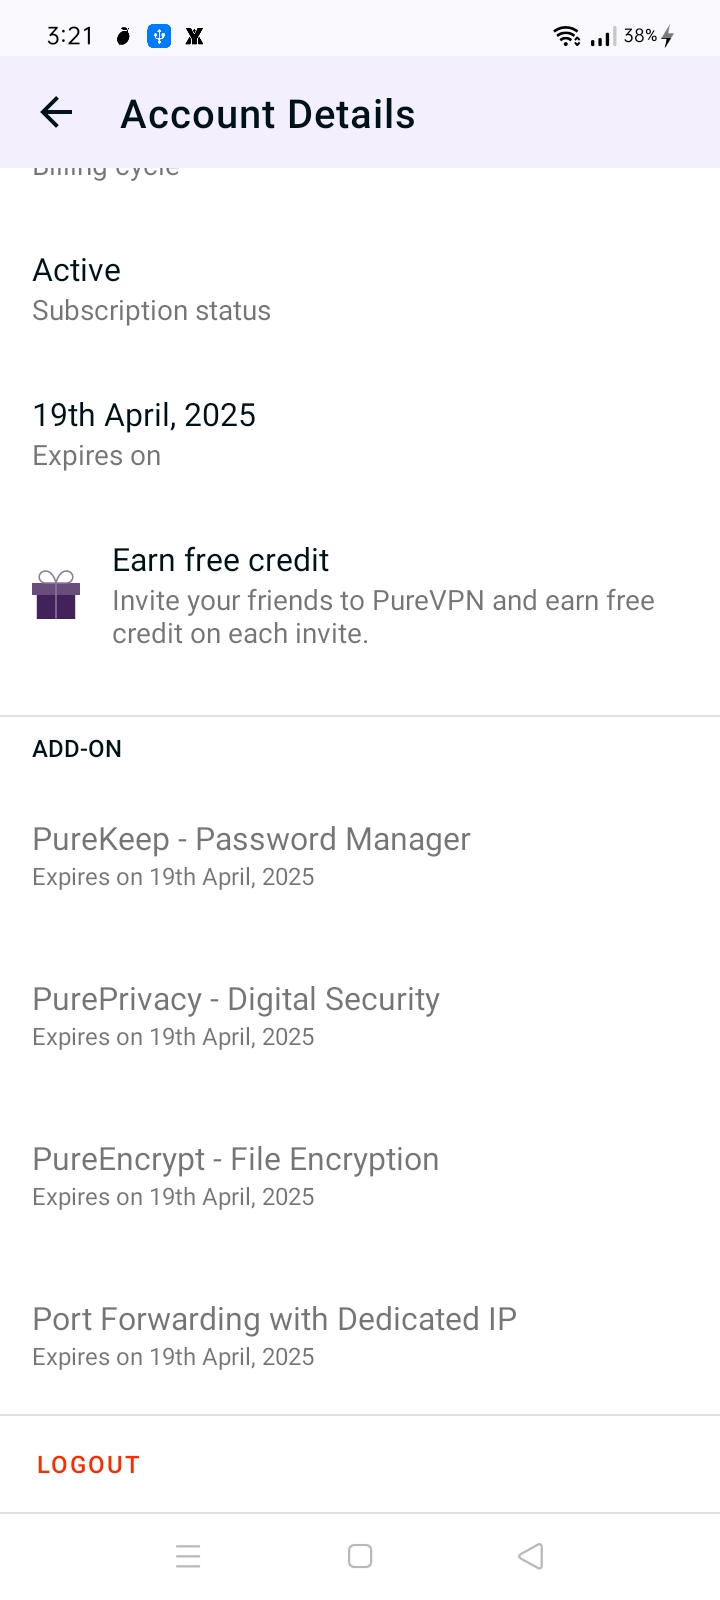
\includegraphics[width=8cm]{39.png}
\centering
\caption{Выйти из системы}
\label{fig:50}
\end{figure}
\item Нажмите Выйти из системы, чтобы продолжить:  Рисунок(\ref{fig:51})
\begin{figure}[H]
\includegraphics[width=8cm]{40.png}
\centering
\caption{Кнопка "Выйти"}
\label{fig:51}
\end{figure}
\item Ваш браузер по умолчанию будет запущен автоматически, и вы получите сообщение с подтверждением того, что вы успешно вышли из приложения PureVPN:  Рисунок(\ref{fig:52})
\begin{figure}[H]
\includegraphics[width=8cm]{34.png}
\centering
\caption{Успешный выход из приложения}
\label{fig:52}
\end{figure}
\end{itemize}

\subsection{Проверьте информацию о подписке в приложении Pure VPN} 
Следуйте приведенным ниже инструкциям, чтобы иметь возможность просматривать данные о вашей подписке в приложении PureVPN.
\begin{itemize}
\item Коснитесь значка гамбургера в левом верхнем углу:  Рисунок(\ref{fig:53})
\begin{figure}[H]
\includegraphics[width=8cm]{35.png}
\centering
\caption{Значок гамбургера}
\label{fig:53}
\end{figure}
\item Коснитесь данных учетной записи:  Рисунок(\ref{fig:54})
\begin{figure}[H]
\includegraphics[width=8cm]{38.png}
\centering
\caption{Данные учетной записи}
\label{fig:54}
\end{figure}
\item В разделе профиля вы сможете просмотреть детали подписки.
\item Ниже приведены подробности, которые будут видны в разделе профиля:  Рисунок(\ref{fig:55})
\begin{enumerate}
\item Имя пользователя VPN
\item Электронная почта
\item Тип подписки
\item Цикл выставления счетов
\item Статус подписки
\item Срок действия подписки истек
\item Дополнение
\end{enumerate}

\begin{figure}[H]
\includegraphics[width=8cm]{41.png}
\centering
\caption{Сведения о подписке}
\label{fig:55}
\end{figure}
\end{itemize}

\section{IOS}

\subsection{Загрузите и установите приложение PureVPN} 
Чтобы загрузить и установить приложение PureVPN, выполните следующие действия:
\begin{itemize}
\item Для начала найдите на своем устройстве приложение App Store и откройте его:  Рисунок(\ref{fig:56})
\begin{figure}[H]
\includegraphics[width=8cm]{42.png}
\centering
\caption{App Store}
\label{fig:56}
\end{figure}

Введите PureVPN в строку поиска и выберите первый результат, который появится в списке.
\item Нажмите получить, как только найдете нужное:  Рисунок(\ref{fig:57})
\begin{figure}[H]
\includegraphics[width=8cm]{43.png}
\centering
\caption{Кнопка получить}
\label{fig:57}
\end{figure}
\item Приложение PureVPN для iOS теперь успешно установлено на ваш телефон:  Рисунок(\ref{fig:58})
\begin{figure}[H]
\includegraphics[width=8cm]{44.png}
\centering
\caption{Приложение установлено}
\label{fig:58}
\end{figure}
\end{itemize}

\subsection{Войдите в приложение PureVPN} 
Как только приложение установлено, вы можете приступить к запуску приложения и войти в него.
\begin{itemize}
\item Запустите приложение PureVPN .
\item Коснитесь Есть учетная запись? Вход:  Рисунок(\ref{fig:59})
\begin{figure}[H]
\includegraphics[width=8cm]{45.png}
\centering
\caption{Вход}
\label{fig:59}
\end{figure}
\item Вы будете перенаправлены в ваш браузер по умолчанию для входа в систему.
\item Введите свой адрес электронной почты PureVPN и пароль (используйте адрес электронной почты и пароль, которые вы указали при покупке).
\item После ввода данных учетной записи нажмите Отправить:  Рисунок(\ref{fig:60})
\begin{figure}[H]
\includegraphics[width=8cm]{46.png}
\centering
\caption{Отправить}
\label{fig:60}
\end{figure}
\item Как только вы нажмете отправить, автоматически откроется приложение PureVPN, и вы войдете в приложение.

Примечание:

Если у вас несколько учетных записей, вам будет предложено выбрать свое имя пользователя PureVPN.
\item После завершения вы будете авторизованы в приложении PureVPN:  Рисунок (\ref{fig:61})
\begin{figure}[H]
\includegraphics[width=8cm]{47.png}
\centering
\caption{Главная страница приложения}
\label{fig:61}
\end{figure}
\end{itemize}

\subsection{Выход из приложения PureVPN для iOS} 
Хотите выйти из приложения PureVPN? Нет проблем ..!! Следуйте простым шагам, приведенным ниже.
\begin{itemize}
\item Коснитесь значка гамбургера в левом верхнем углу:  Рисунок(\ref{fig:62})
\begin{figure}[H]
\includegraphics[width=8cm]{47.png}
\centering
\caption{Значок гамбургера}
\label{fig:62}
\end{figure}
\item Коснитесь сведений об учетной записи:  Рисунок(\ref{fig:63})
\begin{figure}[H]
\includegraphics[width=8cm]{48.png}
\centering
\caption{Сведения об учетной записи}
\label{fig:63}
\end{figure}
\item Нажмите Выйти из системы:  Рисунок(\ref{fig:64})
\begin{figure}[H]
\includegraphics[width=8cm]{49.png}
\centering
\caption{Выйти из системы}
\label{fig:64}
\end{figure}
\item Нажмите Выйти из системы, чтобы продолжить:  Рисунок(\ref{fig:65})
\begin{figure}[H]
\includegraphics[width=8cm]{50.png}
\centering
\caption{Подтвердить выход}
\label{fig:65}
\end{figure}
\item Вы успешно вышли из приложения PureVPN.
\end{itemize}

\subsection{Проверьте информацию о подписке в приложении Pure VPN} 
Ищете способ просмотреть сведения о вашей подписке в приложении PureVPN? Следуйте приведенным ниже инструкциям, чтобы иметь возможность просматривать сведения о вашей подписке в приложении PureVPN.
\begin{itemize}
\item Коснитесь значка гамбургера в левом верхнем углу:  Рисунок(\ref{fig:66})
\begin{figure}[H]
\includegraphics[width=8cm]{47.png}
\centering
\caption{Гамбургер}
\label{fig:66}
\end{figure}
\item Коснитесь сведений об учетной записи:  Рисунок(\ref{fig:67})
\begin{figure}[H]
\includegraphics[width=8cm]{47.png}
\centering
\caption{Сведения об учетной записи}
\label{fig:67}
\end{figure}
\item В разделе профиля вы сможете просмотреть сведения о подписке.
\item Ниже приведены подробности, которые будут видны в разделе профиля:  Рисунок(\ref{fig:68})
\begin{enumerate}
\item Электронная почта
\item Имя пользователя VPN
\item Тип подписки
\item Статус подписки
\item Цикл выставления счетов
\item Срок действия подписки истек
\item Аддоны
\end{enumerate}
\begin{figure}[H]
\includegraphics[width=8cm]{49.png}
\centering
\caption{Информация о подписке}
\label{fig:68}
\end{figure}
\end{itemize}

\end{document}
 